\documentclass[12pt,letterpaper]{book}
\usepackage[utf8]{inputenc}
\usepackage[spanish,es-tabla]{babel}
\decimalpoint
\let\cleardoublepage\clearpage
\usepackage{amsmath}
\usepackage{amsfonts}
\usepackage{amssymb}
% \usepackage[T1]{fontspec}
\usepackage{color}
\usepackage{graphicx}
\usepackage{makeidx}
\makeindex
\usepackage{anysize}
\usepackage{anyfontsize}
\usepackage{pdfpages}
\usepackage[x11names,table]{xcolor}
\usepackage{tikz}
\usepackage{tcolorbox}
\tcbuselibrary{skins,breakable,listings,theorems}
\usepackage[hidelinks]{hyperref}
\usepackage[labelfont=bf]{caption}
\captionsetup[table]{labelsep=space}
\captionsetup[figure]{labelsep=space}
\usepackage{listings}
\usepackage{array,ragged2e}
\usepackage[left=2cm,top=2cm,right=2cm,bottom=2cm]{geometry}
\setlength{\parindent}{0cm}
\usepackage[printwatermark]{xwatermark}
\newwatermark[allpages,color=gray!10,angle=45,scale=3,xpos=0,ypos=0]{Borrador}

\tcbset{colback=green!5!white, colframe=gray!10!black, coltitle=green!20!black, 
fonttitle=\bfseries, colbacktitle=white, coltext=gray!30!black}
\addto\captionsspanish{
  \renewcommand{\figurename}{{\bf Figura}}% 
}
\addto\captionsspanish{
  \renewcommand{\chaptername}{{\bf}}% 
}

\usepackage{epigraph}
\usepackage{fontawesome}
\usepackage[Bjornstrup]{fncychap}

% \renewcommand{\familydefault}{\sfdefault}

% Colores
\definecolor{verdep}{RGB}{166,206,58}
\definecolor{ccap}{RGB}{10,10,50}
\definecolor{csec}{RGB}{50,50,100}
\definecolor{csubsec}{RGB}{80,80,120}
\definecolor{header_table_color}{RGB}{200,255,180}
\definecolor{info_color}{RGB}{100,100,200}
\definecolor{csol}{rgb}{0.2,0.8,0.1}
\definecolor{backcode}{rgb}{0.98,0.98,0.99}
\definecolor{crule}{rgb}{0.9,0.9,0.9}
\definecolor{dkgreen}{rgb}{0,0.6,0}
\definecolor{gray}{rgb}{0.5,0.5,0.5}
\definecolor{mauve}{rgb}{0.58,0,0.82}


\newtcolorbox{ejemplo}[2][]
{
  breakable,
  colframe = gray!50,
  colback  = gray!10,
  coltitle = gray!20!black,
  title    =  \faEdit \hspace{5 mm} #2,
}

\newtcolorbox{informacion}[2][]
{
  breakable,
  colframe = blue!5!white,
  colback  = blue!5!white,
  coltitle = blue!80!black,
  title    = \faInfo \hspace{5 mm} #2,
}

\newtcolorbox{recomendacion}[2][]
{
  breakable,
  colframe = green!25,
  colback  = green!10,
  coltitle = green!20!black,
  title    = #2,
}

 \newcommand{\ccol}{>{\centering\tt\arraybackslash}}

% Nuevos comandos

\usepackage{titlesec}%--
% \newcommand{\hsp}{\hspace{5pt}}
% \titleformat{\chapter}[hang]{\huge\bfseries\color{ccap}}
% {\color{verdep}{\vrule height 2.5cm width 1mm}\hsp{\fontsize{100}{5}\selectfont\thechapter}\hsp%
% {\vrule height 2.5cm width 1mm}\hsp{\fontsize{30}{5}\selectfont}}{5pt}{\huge\bfseries}

\titleformat{\section}[hang]{\normalfont\color{csec}}%
{\filright\large\enspace\thesection\enspace}%
{8pt}{\Large\bfseries\filright}%

\titleformat{\subsection}[hang]{\normalfont\color{csec}}%
{\filright\large\enspace\thesubsection\enspace}%
{8pt}{\large\bfseries\filright}%

% Code

% Code

\lstnewenvironment{matlab}{\lstset{frame=single,
  frameround=tttt,
  backgroundcolor=\color{backcode},
  rulecolor=\color{crule},
  language=matlab,
  aboveskip=5mm,
  belowskip=5mm,
  showstringspaces=false,
  columns=flexible,
  basicstyle={\small\ttfamily},
  numbers=none,
  numberstyle=\tiny\color{gray},
  keywordstyle=\color{blue},
  commentstyle=\color{dkgreen},
  stringstyle=\color{mauve},
  breaklines=true,
  breakatwhitespace=true,
  tabsize=4,
  extendedchars=true,
  inputencoding=utf8,
  literate=%
  {°}{{\,\,$^\circ$\,\,}}1
  {á}{{\'a}}1
  {é}{{\'e}}1
  {í}{{\'i}}1
  {ó}{{\'o}}1
  {ú}{{\'u}}1
  {Á}{{\'A}}1
  {É}{{\'E}}1
  {Í}{{\'I}}1
  {Ó}{{\'O}}1
  {Ú}{{\'U}}1
}}{}


\author{P.J. De Los Santos}
\title{Programación en MATLAB, fundamentos y aplicaciones}

\begin{document}

% 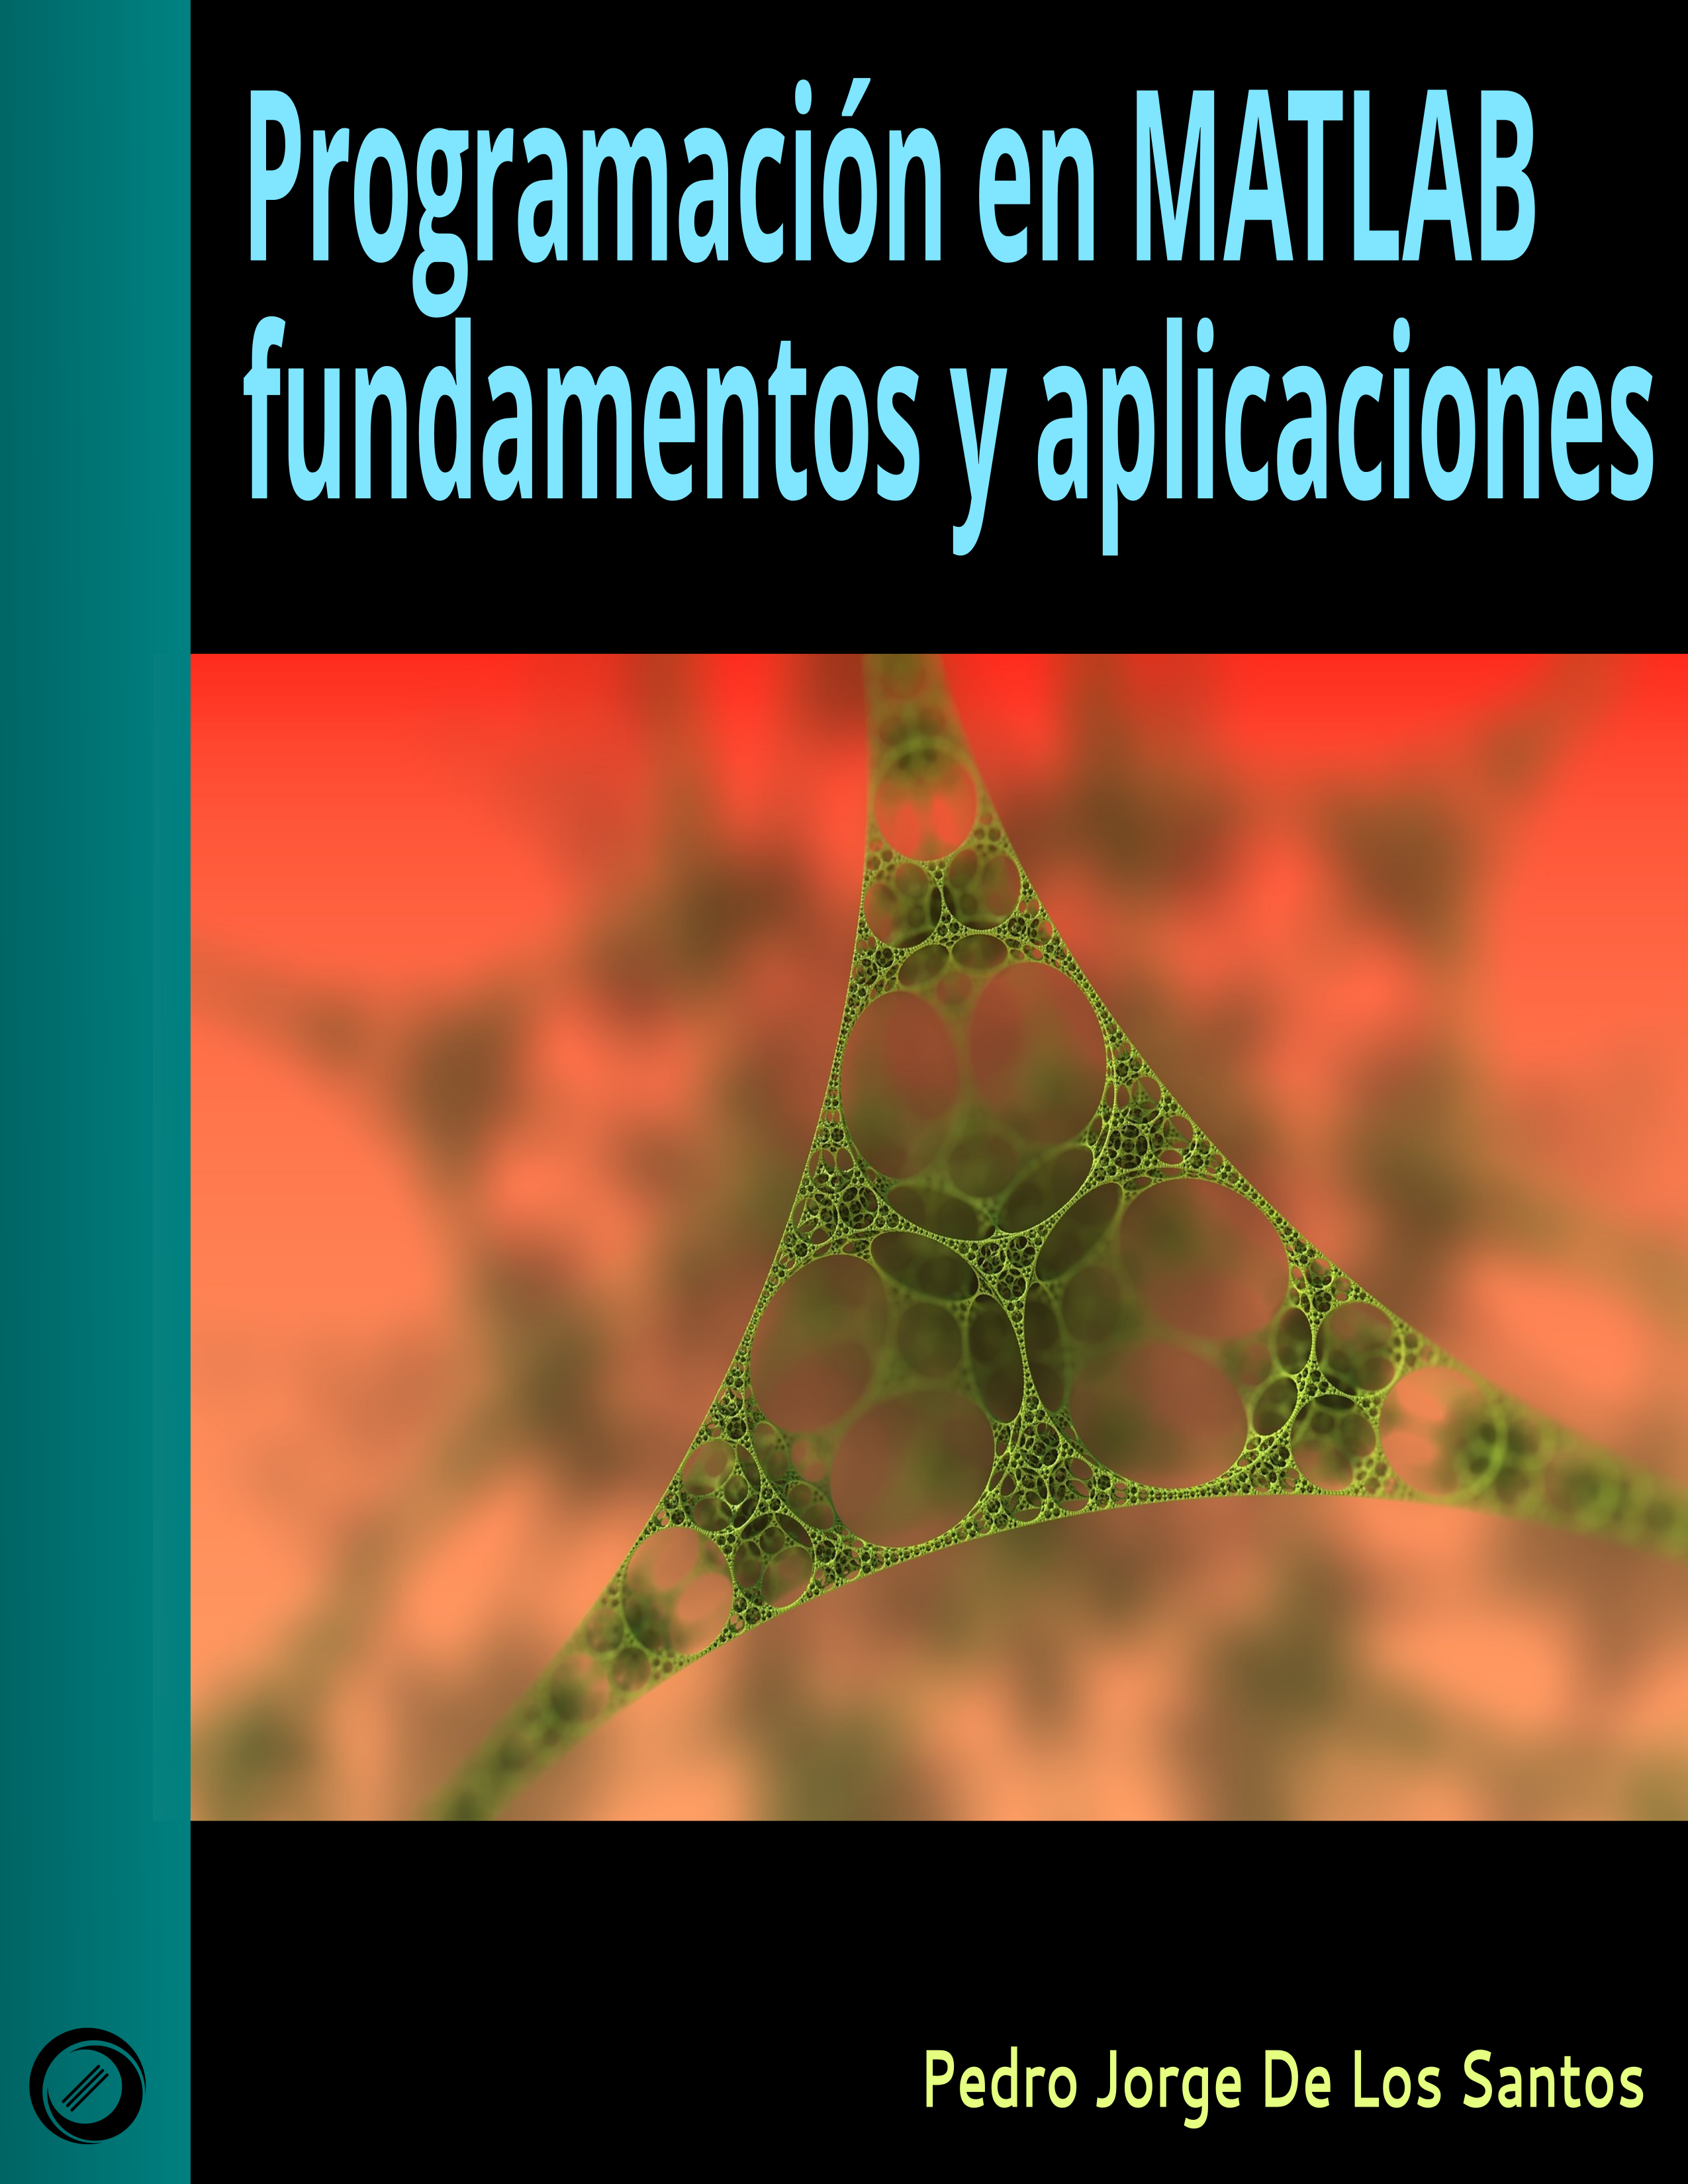
\includepdf{images/title_page.pdf}
\maketitle
\tableofcontents

% \frontmatter
% \chapter*{Versión incompleta}

Esta es una versión incompleta del libro \textbf{Programación en MATLAB,
fundamentos y aplicaciones}, te agradezco por ser un
\emph{early-reader}, cualquier comentario u observación puedes hacérmela
saber a través de los siguientes medios de contacto.

\begin{itemize}
\tightlist
\item
  \href{delossantosmfq@gmail.com}{E-mail}
\item
  \href{https://twitter.com/pjdlsl}{Twitter}
\end{itemize}

O bien a través de la plataforma de LeanPub en el siguiente
\href{https://leanpub.com/programacionmatlab/email_author/new}{link}.
% \chapter*{Introducción}

\subsection*{Del contenido}

\textbf{Programación en MATLAB®\footnote{\emph{MATLAB® es una marca
  registrada de MathWorks, Inc.}}, fundamentos y aplicaciones} consta,
por ahora, de diez capítulos en los cuales se abordan los temas básicos
de la programación en MATLAB y algunas de sus aplicaciones. Los
capítulos son:

\begin{enumerate}
\item Fundamentos del lenguaje
\item Vectores y matrices
\item Arreglos de celdas, estructuras y cadenas de caracteres
\item Gráficas
\item Exportar e importar variables y datos
\item Matemáticas con MATLAB
\item Procesamiento de imágenes
\item Interfaces gráficas de usuario
\item Programación orientada a objetos
\item Recomendaciones generales
\end{enumerate}

El \textbf{capítulo 1} abarca los temas introductorios al lenguaje,
tales como el uso del entorno de desarrollo, los tipos de datos y
operadores, estructuras de control, ficheros de comandos, funciones, etc.
Se espera que al término del capítulo el lector sea capaza de programar 
scritps de manera estructurada y comprenda la función que desempeña 
cada instrucción escrita. \\

El \textbf{capítulo 2} proporciona información más detallada acerca de
los vectores y matrices, cuya importancia es vital para sacar el máximo
provecho del lenguaje, dado que es ahí donde reside la popularidad que
se ha ganado. Se tratan las operaciones más comunes con estructuras 
matriciales: definición/creación, operaciones aritméticas, indexación, 
rotación y redimensionado. \\

El \textbf{capítulo 3} está destinado a tratar otros tipos de datos más
avanzados, pero que de igual forma juegan un papel muy importante en el
aprendizaje. Las cadenas de caracteres se incluyeron en este capítulo
con la finalidad de hacerlas más visibles, dado que muchas veces se
tiende a subestimar en este tipo de lenguajes. \\

El \textbf{capítulo 4} trata un tema muy importante como son las
gráficas, tanto bidimensionales como tridimensionales. Se tratan los 
tipos de gráficos más comunes: líneas, barras, pastel/tarta, polígonos, 
superficies, curvas tridimensionales, esferas, planos, cilindros, y 
por supuesto, algunos temas referentes al \textit{formateo} de las gráficas, 
tales como anotaciones-textos, leyendas, etiquetas, mapas de color, estilos, 
etc.\\

El \textbf{capítulo 5} se ha orientado a las diversas formas de
interactuar con datos contenidos en formatos de aplicaciones externas,
así como el manejo de las variables creadas durante una sesión de
MATLAB, y claro, la manipulación de archivos y directorios utilizando
funciones nativas de MATLAB. \\

El \textbf{capítulo 6} aborda temas fundamentales de matemáticas, tales
como álgebra elemental, cálculo diferencial e integral, cálculo
vectorial, álgebra lineal y ecuaciones diferenciales, estos desde un
enfoque de la computación simbólica. \\

El \textbf{capítulo 7} es una introducción al procesamiento digital de
imágenes, con ejemplos muy simples de lectura/escritura de imágenes
básica, conversión entre modelos de color, operaciones aritméticas,
binarización, detección de bordes, entre otras cuestiones elementales. \\

El \textbf{capítulo 8} es una introducción al desarrollo de interfaces
gráficas de usuario en MATLAB, se abarcan los controles básicos y se
programación utilizando código puro, además de una introducción muy
somera al entorno de desarrollo integrado (GUIDE). \\

El \textbf{capítulo 9} aborda un tópico que generalmente se omite en la
mayoría de los libros de esta especie: la programación orientada a
objetos (POO). Se exponen los conceptos básicos de este paradigma de
programación, la sintaxis correspondiente al lenguaje, la organización
de ficheros de clases y el manejo de objetos. \\
 
El \textbf{capítulo 10} incluye una serie de recomendaciones que le
permitirán al programador en MATLAB el desarrollo de aplicaciones mejor
documentadas, legibles y optimizadas. \\

\subsection*{El por qué...}

Estos apuntes (o algo parecido) han nacido con la finalidad de
proporcionar una herramienta didáctica a quienes inician en el mundo de
la programación en MATLAB. Ciertamente este texto no es un libro
introductorio de programación y hay conceptos elementales que se
consideran asimilados por el lector. Sí es introductorio en lo que
respecta a sintaxis y las formas de implementar soluciones utilizando
MATLAB. Además, la idea es formar unos apuntes colaborativos, en donde
las ideas o comentarios que el lector pudiera retroalimentar sirvan para
mejorar la edición permanente que actualmente tienen estos apuntes.

\subsection*{Portada}

La imagen de portada fue obtenida de
\href{https://pixabay.com/es/nano-tecnolog\%C3\%ADa-construcci\%C3\%B3n-1480553/}{Pixabay},
el autor es Pete Linforth y está publicada bajo licencia
\href{https://creativecommons.org/publicdomain/zero/1.0/deed.es}{CC0 1.0
Universal}.


\begin{verbatim}

P.J. De Los Santos
Celaya, Guanajuato, México.
\end{verbatim}



\mainmatter
% \chapter{Fundamentos del lenguaje}
 
\section{¿Qué es MATLAB?}

MATLAB es un lenguaje de programación de alto nivel y entorno de
desarrollo interactivo, utilizado para numerosas aplicaciones de
carácter técnico y científicas. MATLAB permite realizar adquisición y
análisis de datos, desarrollo de algoritmos computacionales, creación y
simulación de modelos físicos y la visualización gráfica de procesos
determinados. Entre los campos de uso de MATLAB se incluyen el
procesamiento digital de señales, audio, imágenes y vídeo, sistemas de
control, finanzas computacionales, biología computacional, redes
neuronales, etc. \\

\emph{Características del lenguaje:} 

\begin{itemize}
\item
  Interpretado: Esta característica le convierte en un lenguaje no muy
  apto para aplicaciones donde la rapidez de ejecución sea crítica, pero
  esto mismo facilita la depuración de errores y permite un tiempo de
  desarrollo reducido en comparación a los lenguajes compilados
  tradicionales como C/C++.
\item
  Tipado dinámico: No es necesario declarar el tipo de variable a
  utilizar, MATLAB reconoce de forma automática el tipo de dato con el
  que trabajará, aunque claro que es posible declarar un tipo de dato de
  forma explícita utilizando las funciones de conversión adecuadas.
\item
  Multiplataforma: MATLAB está disponible para las plataformas más
  comunes: Unix, Windows, GNU/Linux y Mac OS.
\item
  Multiparadigma: Soporta programación imperativa, funcional y orientada
  a objetos.
\end{itemize}

\section{Descripción del entorno de desarrollo}

El entorno de MATLAB mostrado en la figura \ref{fig:screen_2012b}
pertenece a la versión 2012b, si dispone de otra versión quizá
encontrará cambios significativos en la interfaz, pero los componentes
más importantes permanecen invariables. \\

Como puede observarse en la figura \ref{fig:screen_2012b}, se
distinguen cuatro componentes en el escritorio del entorno MATLAB, los
cuáles son: \\

\textbf{Command Window} \\

Ventana de comandos interactiva en la cual deberán introducirse las
instrucciones de MATLAB, el prompt \verb|>>| le indica que está listo para 
recibir instrucciones. \\

\begin{informacion}{¿Qué es el prompt?}
En la jerga informática, se denomina prompt al símbolo o
caracter que aparece en una terminal o consola, cuando
esta se encuentra en disposición de aceptar un comando
de entrada.
\end{informacion}

\textbf{Current Folder} \\

Carpeta en la que se está situado, y en la que MATLAB buscará y guardará
(por defecto) los archivos generados durante la sesión. \\

\textbf{Workspace} \\

Ventana que muestra las variables creadas por el usuario durante la
sesión, indicando el nombre, valor y tipo de la misma. \\

\textbf{Command History} \\

Permite buscar comandos introducidos con anterioridad en la ventana de
comandos y ejecutarlos nuevamente o copiarlos. \\

\begin{center}
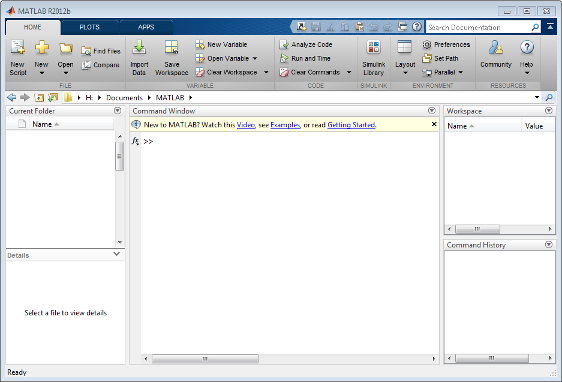
\includegraphics[width=0.8\textwidth]{src/img/ch1/img_1_1.png}
\captionof{figure}{Pantalla de MATLAB R2012b}
\label{fig:screen_2012b}
\end{center}

\section{Comandos básicos y generalidades}

\subsection{Consultar ayuda de MATLAB}

Uno de los puntos fuertes de MATLAB es la extensa documentación que
viene adjunta al software, la cual contiene múltiples ejemplos y
recomendaciones para la mayoría de las funciones. Puede acceder a la
ayuda ubicando el ícono característico de ayuda, o bien tecleando la
instrucción doc en la línea de comandos.\\

Si requiere una referencia rápida acerca de un comando o función puede
utilizar el comando \texttt{help} seguido por el nombre la función a
consultar, lo anterior le mostrará en la ventana de comandos una
descripción breve referente a la función consultada, por ejemplo la
siguiente línea le permite consultar ayuda rápida acerca del comando
\texttt{clc}:

\begin{matlab}
>> help clc
    clc    Clear command window.
    clc clears the command window and homes the cursor.
    See also home.
    Reference page in Help browser
    doc clc
\end{matlab}

\subsection{Limpiar ventana de comandos y variables del workspace}

Generalmente se considera una buena práctica de programación en MATLAB
iniciar los programas con instrucciones de limpiar la consola (Command
Window) y borrar las variables de la memoria. Lo anterior se logra
utilizando las instrucciones \texttt{clc} para limpiar la ventana de
comandos y \texttt{clear} para borrar las variables del workspace. Suele
acompañarse a la instrucción \texttt{clear} con el argumento adicional
\texttt{all}, que permite borrar incluso variables globales, es decir
conjuntamente: \texttt{clear all.}

\subsection{Líneas de comentarios}

Los comentarios de una sola línea en MATLAB deben comenzar con el
símbolo de porcentaje \%, todo aquello escrito después de este símbolo
será ignorado por el intérprete y reconocido como comentario,
asignándosele un color verde característico de forma automática.

\begin{matlab}
% Esto es un comentario en MATLAB
\end{matlab}

Para hacer bloques de comentarios (o comentarios multilínea) MATLAB dispone 
de una sintaxis específica que se muestra enseguida:

\begin{matlab}
%{
Esto es un comentario de múltiples
líneas en MATLAB, delimitado por 
llaves conjuntas con el signo % 
%}
\end{matlab}

\subsection{Valores especiales}\label{valores-especiales}

En la siguiente tabla se resumen algunos valores especiales
\emph{devueltos} por funciones predefinidas en MATLAB:

\begin{table}[h!]
\centering
% \rowcolors{1}{}{gray!20}
\begin{tabular}{p{3cm} p{12cm}}
\hline
\Centering\bfseries Función & \Centering\bfseries Descripción \\
\hline
\texttt{ans} & Guarda el ultimo valor no asignado a una variable \\
\texttt{eps} & Tolerancia que MATLAB soporta en los cálculos \\
\texttt{intmax} & Máximo valor entero que puede utilizarse \\
\texttt{intmin} & Mínimo valor entero que puede utilizarse \\
\texttt{realmax}  & Valor de coma flotante máximo que puede representarse \\
\texttt{realmin} & Valor de coma flotante mínimo que puede representarse \\
\texttt{pi} & Constante matemática (3.14159265…) \\
\texttt{inf} & Valor asignado a un número demasiado grande respecto a la
capacidad de cálculo del software. \\
\texttt{NaN} & Iniciales de “Not a Number”, tal cual traducción literal hace
referencia a un valor numérico inválido. \\
\texttt{computer} & Devuelve el tipo de computadora que se está utilizando\\
\texttt{version} & Devuelve la versión de MATLAB \\
\hline
\end{tabular}
\caption{Valores especiales}
\end{table}

\section{Tipos de datos y operadores}

El siguiente listado resume los tipos de datos más comunes en MATLAB:

\begin{itemize}
\item logical  (tipo booleano o lógico)
\item char (cadenas de caracteres)
\item numeric (datos tipo numérico)
\begin{itemize}
   \item int8, int16, int32, int64 (tipos entero)
   \item uint8, uint16, uint32, uint64  (enteros sin signo)
   \item single (flotantes de precisión simple)
   \item double  (flotantes de precisión doble)
\end{itemize}
\item cell (arreglos de celdas)
\item struct (estructuras)
\end{itemize}

\subsection{Tipo logical}

El tipo de dato lógico o booleano es en computación aquel que puede 
representar valores de lógica binaria, esto es 2 valores, valores 
que normalmente representan falso o verdadero. \\

En MATLAB las variables de tipo lógico permiten, evidentemente, dos valores, que
pueden ser \texttt{true} o \texttt{false}. Una forma de declarar una
variable de tipo lógico sería:

\begin{matlab}
>> a = true
a =
     1
\end{matlab}

Otra manera que resulta en lo mismo es la siguiente:

\begin{matlab}
>> a=logical(1)
a =
     1
\end{matlab}

Las líneas anteriores crean una variable \texttt{a} de tipo lógico con
un valor \texttt{true}. \\

La utilidad de los variables lógicas se hace evidente cuando es necesario 
tomar decisiones respecto al estatus o valor de una variable o subrutina.

\subsection{Tipo char}

Son cadenas de caracteres, que pueden contener valores alfanuméricos e
incluso símbolos especiales. Para declararlas no hace falta especificar
que son variables tipo \texttt{char}, dado que MATLAB es de tipado dinámico y
reconoce como tal aquellas cuyo valor asignado se encuentre delimitado
por comillas simples, un ejemplo muy clásico es el siguiente:

\begin{matlab}
>> txt = 'Hola Mundo'
txt =
Hola Mundo
\end{matlab}

El manejo de cadenas de caracteres o strings es una cuestión fundamental 
en la programación de computadoras. En MATLAB las cadenas de caracteres 
tienen muchas utilidades, entre las cuales pueden citarse: sirven como 
argumentos de entrada para funciones (como todo tipo de dato), identificadores 
para campos de estructuras, anotaciones y etiquetas en las gráficas, 
lectura y escritura de datos no uniformes, entre muchas otras. \\

En el capítulo 3 se aborda el manejo de strings de una manera muy completa, 
desde operaciones básicas como las comparaciones y concatenación, hasta el 
uso de expresiones regulares.

\subsection{Tipo numeric}

Normalmente cuando en MATLAB tecleamos un valor numérico o bien lo
asignamos a una determinada variable, esta será de tipo double, a menos
que se haga una conversión explicita a otro tipo de dato. Por ejemplo,
si insertamos en MATLAB lo siguiente:

\begin{matlab}
>> num = 10
num =
    10
\end{matlab}

Y posteriormente tecleamos la instrucción \texttt{whos} para verificar 
el tipo o clase de dicha variable:

\begin{matlab}
>> whos
  Name      Size            Bytes  Class     Attributes
  num       1x1                 8  double   
\end{matlab}

Si se requiere utilizar un dato de tipo entero habrá de realizarse la
conversión como sigue:

\begin{matlab}
>> numInt = int8(23)
numInt =
   23
>> whos
  Name        Size            Bytes  Class    Attributes
  numInt      1x1                 1  int8               
\end{matlab}

\subsection{Tipo cell}

Un cell array es un tipo de dato característico del lenguaje MATLAB que
consiste en un arreglo multidimensional de celdas que pueden contener
cualquier tipo de dato, inclusive otro cell array. Un ejemplo muy
sencillo de cell array se muestra enseguida:

\begin{matlab}
>> C={10,'MATLAB','5',[1 1]}
C = 
    [10]    'MATLAB'    '5'    [1x2 double]
\end{matlab}

\subsection{Tipo struct}\label{tipo-struct}

Las estructuras son arreglos de datos que, de forma similar a los cell
arrays, pueden almacenar variables de diversos tipos. Para la
organización de los datos se utilizan campos que pueden contener sólo un
tipo de dato. A continuación se muestra un ejemplo de cómo crear una
estructura:

\begin{matlab}
>> Alumno.Nombre='Jorge';
>> Alumno.Apellido='De Los Santos';
>> Alumno.Cursos={'Programación','Cálculo','Métodos Numéricos'};
>> Alumno.Notas=[10 9 10];
>> Alumno
Alumno = 
      Nombre: 'Jorge'
    Apellido: 'De Los Santos'
      Cursos: {'Programación'  'Cálculo'  'Métodos Numéricos'}
       Notas: [10 9 10]
\end{matlab}

En el capítulo 3 se tratan con más detenimiento las estructuras y su
utilidad en la programación en MATLAB.

\subsection{Referencias de función (function handle)}\label{referencias-de-funcion-function-handle}

Las \emph{function handle} son referencias asociadas a una función
nativa de MATLAB o bien a una función anónima creada por el usuario.\\

El siguiente ejemplo muestra la definición de una función anónima y su
posterior uso mediante su referencia:

\begin{matlab}
>> f=@(x) x+cos(x)
f = 
    @(x)x+cos(x)
>> whos
  Name      Size            Bytes  Class              Attributes
  f         1x1                32  function_handle              
>> fzero(f,0) % Raíz de la función 
ans =
   -0.7391
>> f(pi/2) % Evaluando función en un punto
ans =
    1.5708
\end{matlab}

\subsection{Identificar tipos de datos}

Para identificar tipos de datos en MATLAB se cuentan con diversos
comandos que nos facilitan esta tarea. El comando \texttt{whos} nos
proporciona información acerca de las variables existentes en el
workspace, tales como el nombre, tamaño y tipo. A manera de ejemplo
crearemos las siguientes variables e introducimos la instrucción whos
para verificar el tipo de información que nos imprime en la consola:

\begin{matlab}
>> n=10;
>> val=false;
>> s='MATLAB';
>> C={1,2,3};
>> ST.Nombre='Anna';
>> whos
  Name      Size            Bytes  Class      Attributes
  C         1x3               360  cell                 
  ST        1x1               184  struct               
  n         1x1                 8  double               
  s         1x6                12  char                 
  val       1x1                 1  logical      
 
\end{matlab}

Además del comando \texttt{whos}, puede utilizarse la función
\texttt{class} para determinar el tipo de dato de una variable pasada
como argumento, por ejemplo:

\begin{matlab}
>> a=3;
>> class(a)
ans =
double
\end{matlab}

\subsection{Conversiones entre tipos de datos}

Las conversiones entre tipos de datos son muy utilizadas en la
programación en cualquier lenguaje, puesto que permiten controlar la
precisión de los cálculos, mejorar la presentación de los datos o bien
evitar errores en la ejecución.

\subsubsection{Entre tipos numéricos}

Cuando se crea una variable de tipo numérico en MATLAB por defecto será
de tipo \texttt{double}, por ejemplo, creamos una variable llamada \texttt{num}:

\begin{matlab}
>> num=2;
>> class(num)
ans =
double
\end{matlab}

Las conversiones entre tipos numéricos son de sintaxis muy sencilla,
solo habrá que especificar el tipo de dato al cual se convertirá, siendo
permitidos los especificados en la tabla siguiente:

\begin{table}[h!]
\centering
% \rowcolors{1}{}{gray!20}
\begin{tabular}{p{5cm} >{\tt}P{5cm} p{5cm}}
\hline 
\Centering\bfseries Tipo de dato & \Centering\bfseries Sintaxis de conversión & \Centering\bfseries Rango \\
\hline
Precisión doble & double(num) & 2.2251e-308 a 1.7977e+308 \\
Precisión simple & single(num) & 1.1755e-38 a 3.4028e+38 \\
Entero de 8 bits & int8(num) & -128 a 127 \\
Entero de 16 bits & int16(num) & -32768 a 32767 \\
Entero de 32 bits & int32(num) & -231 a 231-1 \\
Entero de 64 bits & int64(num) & -263 a 263-1 \\
Entero sin signo de 8 bits & uint8(num) & 0 a 255 \\
Entero sin signo de 16 bits & uint16(num) & 0 a 65535 \\
Entero sin signo de 32 bits & uint32(num) & 0 a 4294967295 \\
Entero sin signo de 64 bits & uint64(num) & 0 a 18446744073709551615 \\
\hline
\end{tabular}
\caption{Conversiones entre tipos numéricos}
\end{table}

Así, podemos convertir la variable num, creada con anterioridad, a otro
tipo de dato numérico, por ejemplo a un entero de 8 bits:

\begin{matlab}
>> num=int8(num);
>> class(num)
ans =
int8
\end{matlab}

Es necesario poner especial atención en los rangos que pueden
manipularse con cada tipo numérico, debido a que por ejemplo si se
realiza la siguiente conversión:

\begin{matlab}
>> num=int8(653)
num =
  127
\end{matlab}

El valor que ha sido pasado como argumento de conversión excede el rango
para un entero de 8 bits, por lo cual simplemente se le asigna el máximo
valor permitido para una variable de este tipo. \\

Si requiere verificar por usted mismo los valores máximos y mínimos
permitidos para cada tipo de dato, puede usar las funciones
\texttt{realmin} y \texttt{realmax} para los tipos de coma flotante, y
las correspondientes \texttt{intmin} e \texttt{intmax} para tipos
enteros.

\subsubsection{De string a tipo numérico}

Para este tipo de conversiones MATLAB dispone de la funciones
\texttt{str2double} y \texttt{str2num}, en algunos casos no notará la
diferencia en los resultados, salvo en la rapidez de ejecución. Pese a
lo anterior, es necesario tomar en cuenta cómo trabaja cada función y
cual le resulta de utilidad; con \texttt{str2double} se convierte una
variable tipo string en un valor de tipo double, la función
\texttt{str2num} también realiza conversión a tipo double pero además
realiza conversiones a otros tipos de datos numéricos si se especifica
de manera explícita, de hecho esta tiene una funcionalidad muy similar a
la de la función \texttt{eval}. Los siguientes ejemplos muestran las
diferencias y utilidades de las funciones descritas.

\begin{matlab}
>> a=str2double('1237')
a =
        1237
>> b=str2num('1237')
b =
        1237
>> whos
  Name      Size            Bytes  Class     Attributes
  a         1x1                 8  double              
  b         1x1                 8  double     
\end{matlab}

\subsection{Operadores aritméticos, relacionales y lógicos}

Los operadores son símbolos especiales fundamentales en un lenguaje de
programación, se utilizan para \emph{operar} sobre variables
(operandos) y, de manera general, pueden clasificarse en tres grupos:

\begin{itemize} 
\item Operadores aritméticos
\item Operadores relacionales
\item Operadores lógicos
\end{itemize}

\subsubsection{Operadores aritméticos}

Los operadores aritméticos toman valores numéricos como entrada y
devuelven un valor resultante de aplicar la operación correspondiente
sobre los operandos. Por ejemplo, vea la siguiente expresión que
corresponde a una suma de escalares:

\begin{matlab}
>> 1+2
ans =
     3
\end{matlab}

En este caso \texttt{1} y \texttt{2} son los operandos o valores sobre
los cuales se aplica el operador \texttt{+}, y \texttt{3} es,
evidentemente, el resultado de ejecutar la operación. \\

En la siguiente tabla se listan los principales operadores aritméticos
disponibles en MATLAB.

\begin{table}[h!]
\centering
% \rowcolors{1}{}{gray!20}
\begin{tabular}{>{\tt}P{3cm} p{9cm}}
\hline
\normalfont\bfseries Operador  & \Centering\bfseries Descripción \\
\hline
+ & Operador  suma \\
- & Operador resta \\
* & Operador multiplicación (escalares) \\
/ & Operador división \\
./ & División elemento a elemento (matrices) \\
.* & Multiplicación elemento a elemento (matrices) \\
\hline
\end{tabular}
\caption{Operadores aritméticos}
\end{table}

Note que además de los operadores correspondientes a las operaciones
aritméticas básicas (suma, resta, multiplicación, división,
potenciación), se tiene operadores que realizan operaciones elemento a
elemento, que se utilizan para operar sobre arreglos matriciales.\\

Por ejemplo, sean \texttt{A} y \texttt{B} dos matrices de 3x3 definidas
como

$$
A = \begin{pmatrix}
1 & 2 \\
3 & 4 \\
\end{pmatrix}
\,\,\,\,\,\,\,\,\,\,\,\,
A = \begin{pmatrix}
5 & 6 \\
7 & 8 \\
\end{pmatrix}
$$

Si realizamos una suma o resta con estas matrices no habrá mayor
complicación, dado que tanto la suma y resta matricial se realizan
elemento a elemento:

\begin{matlab}
>> A=[1,2;3,4];
>> B=[5,6;7,8];
>> A+B
ans =
     6     8
    10    12
>> A-B
ans =
    -4    -4
    -4    -4
\end{matlab}

Luego, note las diferencias de utilizar la multiplicación elemento a
elemento (\texttt{.*}) y la ordinaria (\texttt{*}):

\begin{matlab}
>> A*B
ans =
    19    22
    43    50
>> A.*B
ans =
     5    12
    21    32
\end{matlab}

Sí, efectivamente los resultados son completamente diferentes: en el
primer caso se realiza una
\href{https://es.wikipedia.org/wiki/Multiplicaci\%C3\%B3n_de_matrices}{multiplicación
matricial}, siguiendo las reglas dictadas por el álgebra de matrices, en
el segundo caso lo que se hace es una multiplicación elemento a
elemento, es decir, cada elemento en la posición $(i,j)$ de
$\bf{A}$ se multiplica con el elemento ubicado en la misma
posición de $\bf{B}$.

\subsubsection{Operadores relacionales}\label{operadores-relacionales}

Los operadores relacionales se utilizan para comparar dos valores,
devolviendo un valor lógico. Normalmente se utilizan en conjunto con las
estructuras de control para la toma de decisiones sobre el procedimiento
o flujo de un programa.\\

La siguiente tabla resume los operadores relacionales: su notación y
descripción.

\begin{table}[h!]
\centering
% \rowcolors{1}{}{gray!20}
\begin{tabular}{P{3cm} p{4cm}}
\hline
\Centering\bfseries Operador  & \Centering\bfseries Descripción \\
\hline 
== & Igual a  \\
$<$ & Menor que \\
$>$ & Mayor que \\
$<$= & Menor o igual que \\
$>$= & Mayor o igual que \\
$\sim =$ & Diferente de \\
\hline
\end{tabular}
\caption{Operadores relacionales}
\end{table}

Puede ver que la notación difiere de la que ordinariamente utilizamos
cuando escribimos en papel, por ejemplo el símbolo del menor o igual
que $\le$ se escribe como \texttt{<=}. Es importante
notar que la comparación ``igual que'' se realiza con un doble signo
igual (\texttt{==}), puesto que el uso de un único signo corresponde a
la asignación, a continuación se muestra lo que ocurre cuando intentamos
hacer comparaciones utilizando sólo un signo \texttt{=}:

\begin{matlab}
>> 1==1
ans =
     1
>> 1=1
 1=1
 |
Error: The expression to the left of the equals sign is not a valid target for an assignment.
\end{matlab}

En el primer caso (doble signo) la comparación se hace devolviendo un
\texttt{true}, pero, en el segundo nos manda un error de sintaxis,
indicando que el \texttt{1} ubicado a la izquierda del signo igual no es
un caracter válido para realizar una asignación.

\subsubsection{Operadores lógicos}


\begin{table}[h!]
\centering
% \rowcolors{1}{}{gray!20}
\begin{tabular}{>{\tt}P{3cm} p{4cm}}
\hline
\normalfont\bfseries Operador  & \Centering\bfseries Descripción \\
\hline
\& & Operador lógico and \\
$|$ & Operador lógico or \\
$\sim$ & Operador lógico not \\
\hline
\end{tabular}
\caption{Operadores lógicos}
\end{table}

\section{Un mini tutorial de introducción}

Una vez conocidos los tipos de datos y los operadores, podemos comenzar
con una breve introducción al uso de MATLAB como una poderosa
calculadora muy fácil de utilizar, además vamos a ver algunas
características interesantes. Si hay algo en esta sección que te parece
díficil de asimilar, no debes preocuparte, lo subsiguiente se abordará
en capítulos posteriores de manera más \emph{detenida}.\\

Como se ha descrito en secciones anteriores, el command window o ventana
de comandos es la parte del entorno MATLAB que nos permite interactuar
de forma dinámica, si tecleamos una instrucción automáticamente nos
devolverá un resultado y se crearán variables en las cuales se almacenen
los diversos valores de salida. Por ejemplo, vamos a teclear una simple
suma aritmética:

\begin{matlab}
>> 3+2
ans =
     5
\end{matlab}

Puede verificar que en el workspace ahora aparece una variable llamada
\texttt{ans} con valor de 5, en \texttt{ans} se guarda por defecto el
último resultado no asignado a una variable, podríamos asignar el
resultado de la suma a una variable específica:

\begin{matlab}
>> suma=3+2
suma =
     5
\end{matlab}

Podemos también asignar valores a determinadas variables y enseguida
utilizarlas para ejecutar alguna operación, por ejemplo:

\begin{matlab}
>> a=5;
>> b=7;
>> a*b
ans =
    35
>> a-b
ans =
    -2
>> a/b
ans =
    0.7143
\end{matlab}

Note que el colocar un punto y coma (;) al final de una instrucción
evita que se muestre un resultado de salida, lo cual no afecta en el
almacenamiento de los valores correspondientes, pero podría resultar de
mucha ayuda al momento de seleccionar los valores que se quieren mostrar
en la ventana de comandos.\\

MATLAB también tiene disponible diversas funciones matemáticas
predefinidas, que pueden ser aplicadas sobre un número o sobre una
matriz o arreglo de números. Algunas funciones trigonométricas:

\begin{matlab}
>> sin(pi/2)
ans =
     1
>> cos(pi/4)
ans =
    0.7071
>> tan(pi/3)
ans =
    1.7321
\end{matlab}

Note que el valor de la constante $\pi$ está predefinida en
MATLAB mediante la cadena \texttt{pi}:

\begin{matlab}
>> pi
ans =
    3.1416
\end{matlab}

MATLAB devuelve un valor de 3.1416, lo cual es un valor
\emph{redondeado} de $\pi$, pero esto es cuestión solamente de
la representación, normalmente se utiliza el formato short (4 dígitos
después del punto decimal) para la representación de valores numéricos,
internamente MATLAB utiliza más digitos para \emph{manejar} y operar con
el valor de $\pi$. Si queremos obtener más digitos en la salida
por consola podemos cambiar el formato de salida:

\begin{matlab}
>> format long
>> pi
ans =
   3.141592653589793
\end{matlab}

El formato largo permite representar una cantidad con 16 decimales.
Incluso es posible \emph{forzar} a que se muestre una representación en
forma racional:

\begin{matlab}
>> format rat
>> pi
ans =
     355/113   
>> 0.1+0.123
ans =
     223/1000  
>> 0.125
ans =
       1/8
\end{matlab}

Se puede crear una lista o arreglo de valores numéricos encerrando estos
entre corchetes, y separando cada elemento por comas o espacios.

\begin{matlab}
>> A=[5,8,10,2,7]
A =
     5     8    10     2     7
>> B=[3 7 1 0 -2]
B =
     3     7     1     0    -2
\end{matlab}

Se puede obtener el valor máximo y mínimo de un arreglo numérico
utilizando las funciones \texttt{max} y \texttt{min} respectivamente.

\begin{matlab}
>> max(A)
ans =
    10
>> min(A)
ans =
     2
\end{matlab}

También podemos calcular el promedio de los valores utilizando la
función \texttt{mean}:

\begin{matlab}
>> mean(A)
ans =
    6.4000
\end{matlab}

Obtener la cantidad de elementos que componen lista con \texttt{length}
o \texttt{numel}:

\begin{matlab}
>> length(A)
ans =
     5
>> numel(A)
ans =
     5
\end{matlab}

Incluso podemos representar gráficamente cada uno de los elementos de un
vector mediante la función \texttt{plot}:

\begin{matlab}
>> x=[1,2,1,3,4,2,0,1];
>> plot(x);
\end{matlab}

\begin{center}
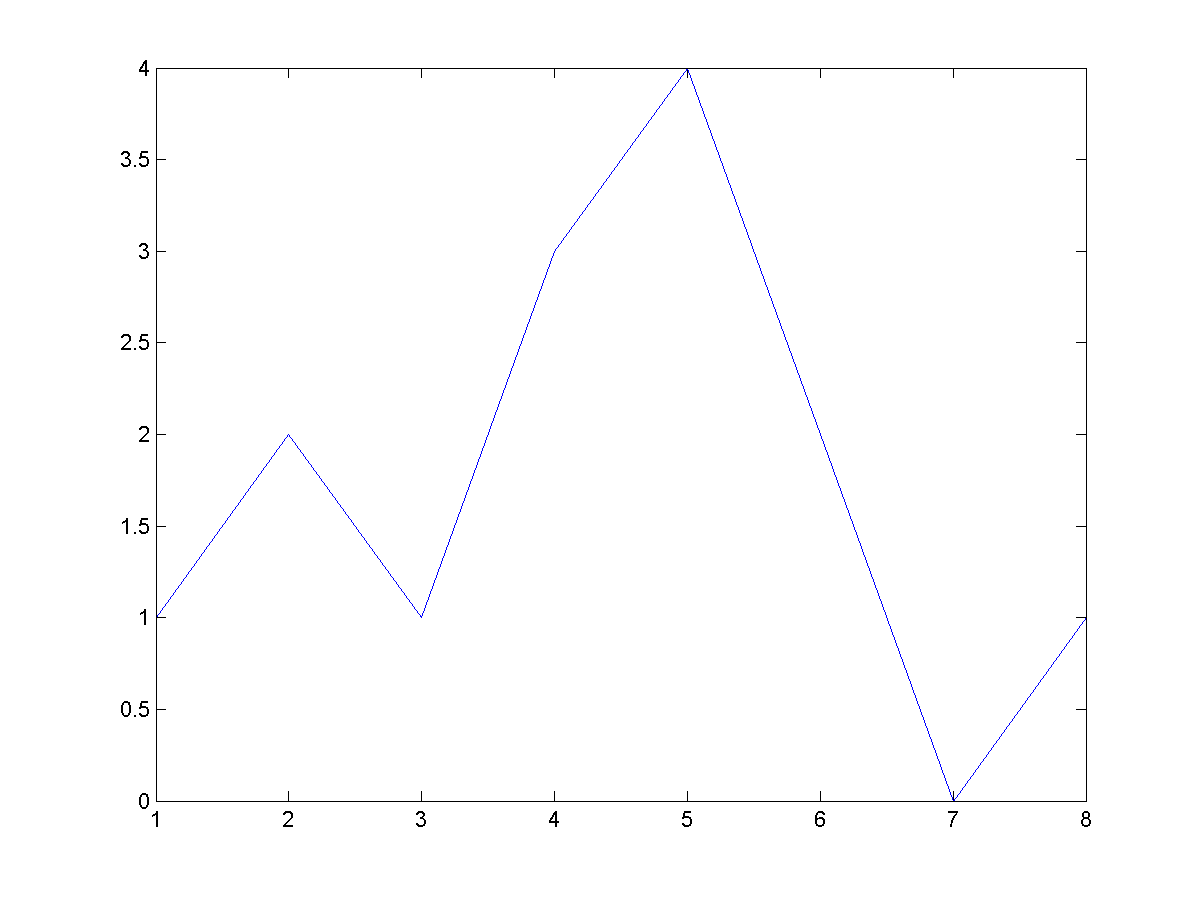
\includegraphics[width=0.6\textwidth]{src/img/ch1/img_1_2.png}
\captionof{figure}{Gráfica de un vector de puntos}
\label{fig:graph_fun}
\end{center}

De manera similar puede evaluar una función matemática en un intervalo
determinado y trazar su gráfica:

\begin{matlab}
>> x=0:0.01:10;
>> y=sin(x);
>> plot(x,y)
\end{matlab}

En lo anterior, se crea un vector \texttt{x} en el intervalo {[}0,10{]},
con incrementos de 0.01, es decir, el vector contiene los puntos:

$$ x = [0, 0.01, 0.02, 0.03,..., 9.99, 10] $$

Luego, al aplicar la función \texttt{sin} sobre ese vector, MATLAB
evalúa la función seno en cada uno de los puntos o valores contenidos en
el arreglo \texttt{x} y los guarda en \texttt{y}. El capítulo 2
(Vectores y matrices) trata con mayor profundidad la notación de dos
puntos utilizada y el manejo correcto de estructuras matriciales.

\begin{center}
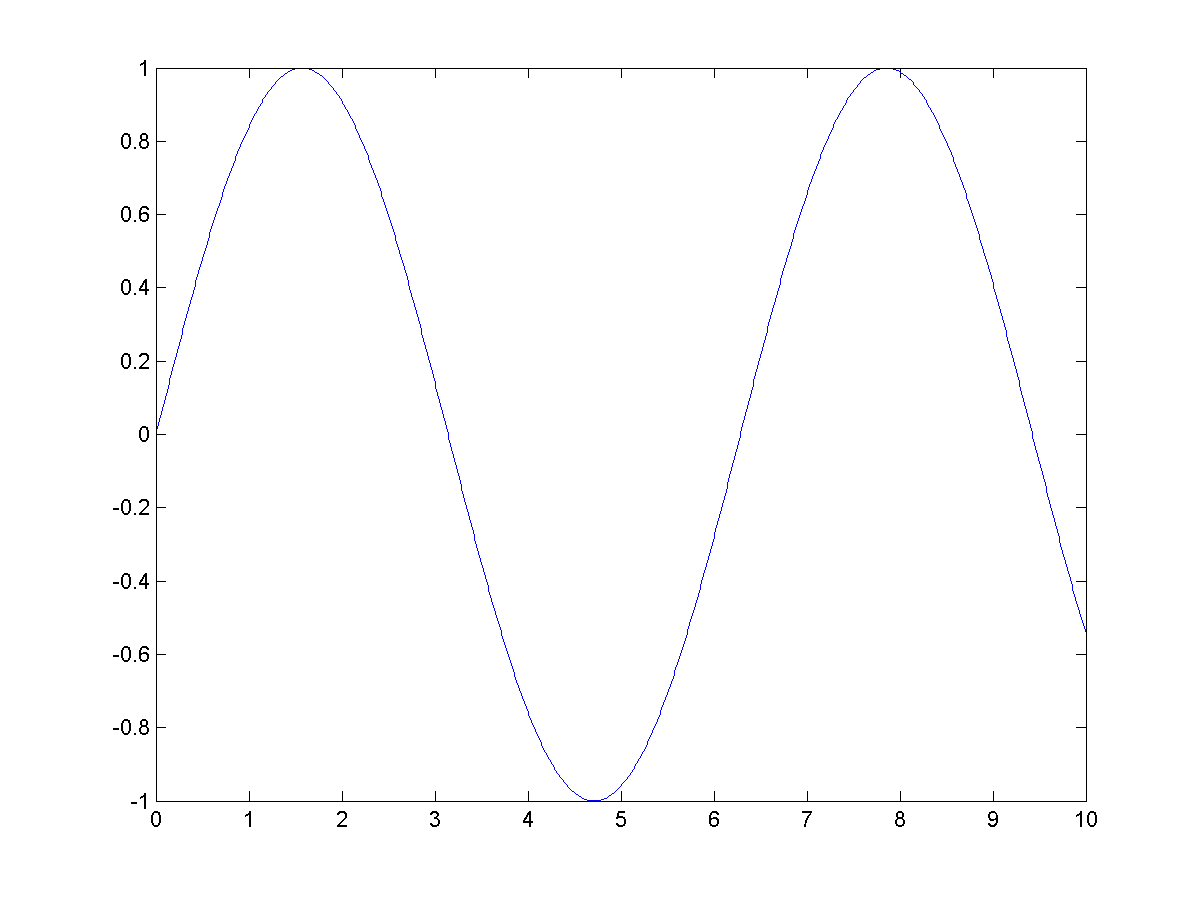
\includegraphics[width=0.6\textwidth]{src/img/ch1/img_1_3.png}
\captionof{figure}{Gráfica de la función $f(x)=\sin{x}$}
\label{fig:gla1}
\end{center}

¿Bastante interesante, verdad?. Bueno, incluso es posible trazar
gráficas de superficies tridimensionales con unas cuantas líneas de
código:

\begin{matlab}
>> [X,Y]=meshgrid(0:0.1:10, 0:0.1:10);
>> Z = sin(X)+cos(Y);
>> surf(X,Y,Z)
\end{matlab}

\begin{center}
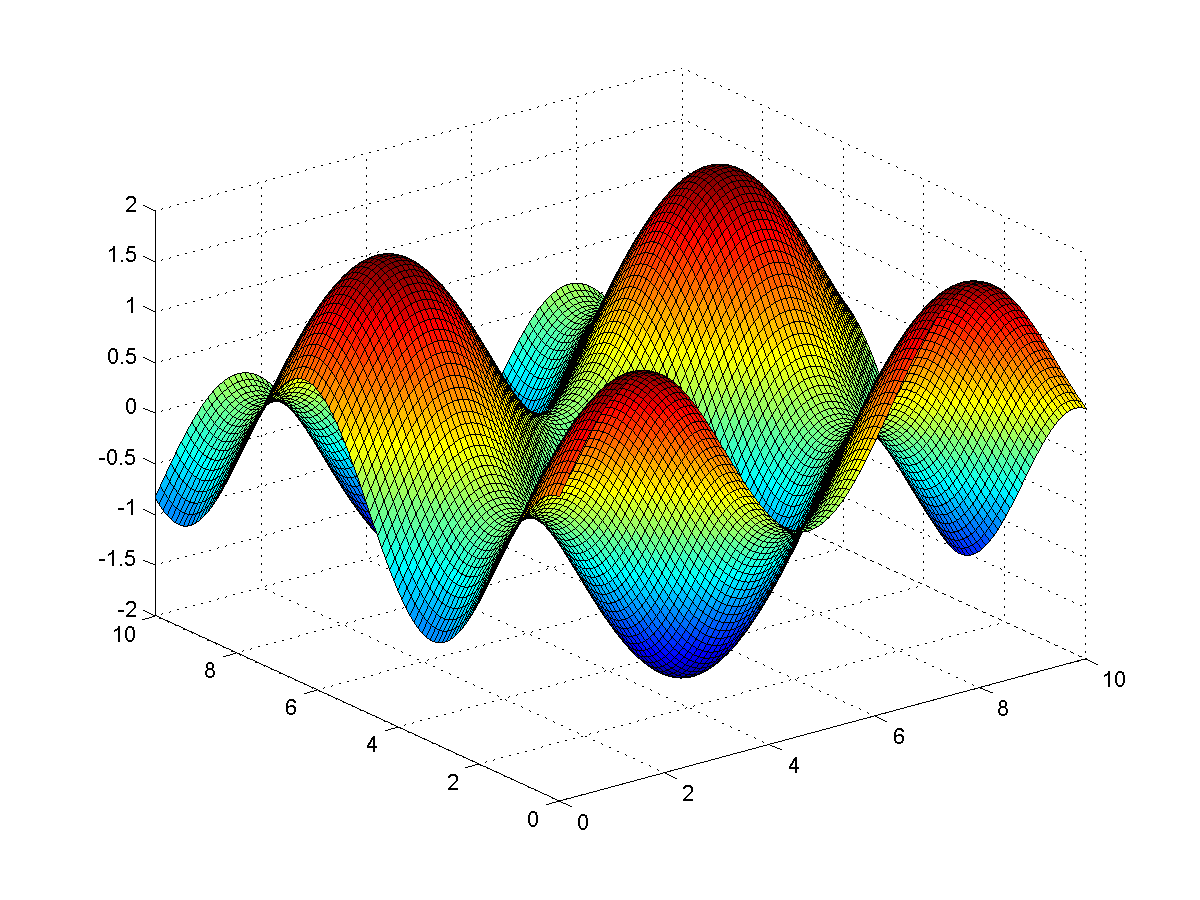
\includegraphics[width=0.6\textwidth]{src/img/ch1/img_1_4.png}
\captionof{figure}{Gráfica de una función $f(x,y)$}
\label{fig:xxxx}
\end{center}

Lo mismo podemos leer una imagen y hacerle algunos cambios
(restauración, segmentación, etc,...) utilizando el \emph{Image
Processing Toolbox} (que es una colección de códigos MATLAB que
facilitan esta tarea). Vea el siguiente ejemplo:

\begin{matlab}
>> img = imread('lena_std.tif');
>> img = rgb2gray(img);
>> filtro = [1 1 1; 1 -8 1; 1 1 1];
>> img_mod = imfilter(img, filtro);
>> imshow(255-img_mod)
\end{matlab}

\begin{center}
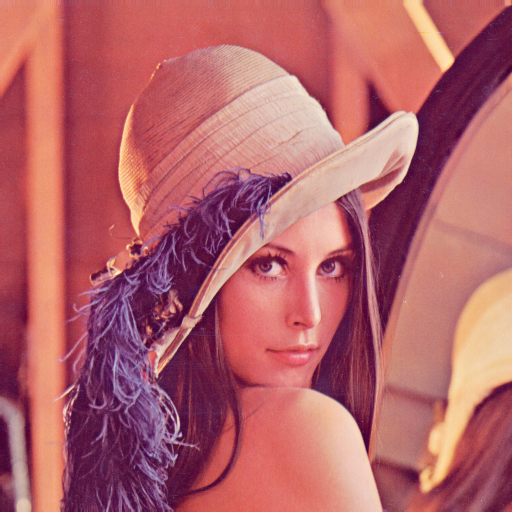
\includegraphics[width=0.4\textwidth]{src/img/ch1/lena.png}
\captionof{figure}{Imagen de Lena original}
\label{fig:lena}
\end{center}

\begin{center}
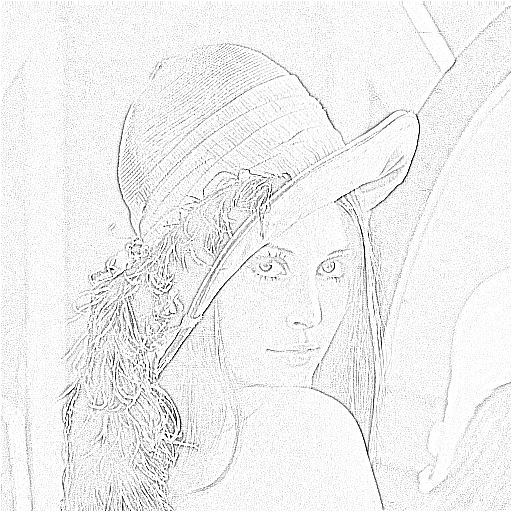
\includegraphics[width=0.4\textwidth]{src/img/ch1/lena_mod.png}
\captionof{figure}{Imagen de Lena modificada}
\label{fig:lena_mod}
\end{center}

Todo esto muestra un poco de lo que puede hacer MATLAB, pero, lo cierto
es que es un entorno muy completo con una \emph{infinidad} de opciones
que facilitan el desarrollo de algoritmos para aplicaciones en múltiples
disciplinas científicas. En los capítulos posteriores de este texto se
abordan algunas características y herramientas proporcionadas por MATLAB
para algunos campos específicos.

\section{Ficheros de comandos (scripts)}

Los ficheros de comandos, conocidos también como \emph{scripts}, son
archivos de texto sin formato (ASCII) con la extensión característica de
los archivos de MATLAB (*.m), se utilizan para almacenar una serie de
comandos o instrucciones que se ejecutan sucesivamente y que habrán de
realizar una tarea específica. Los scripts de MATLAB pueden editarse
utilizando cualquier editor de texto sin formato (Bloc de Notas,
Notepad++, Sublime Text, etc\ldots{}), aunque es más recomendable
utilizar el editor de MATLAB, puesto que proporciona herramientas que
facilitan la corrección de errores, el control sobre la ejecución del
código y la capacidad de autocompletado y sugerencias cuando se utilizan
funciones nativas de MATLAB.\\

Para crear un nuevo script puede pulsar la combinación \textbf{Ctrl + N}
(bajo SO Windows), o buscar en la interfaz de MATLAB la opción New y
enseguida seleccionar Script; si prefiere hacerlo desde la ventana de
comandos puede introducir el comando edit que le abrirá un nuevo script.\\

Para guardar un fichero de comandos utilice la opción \textbf{Save} de
la barra de herramientas o bien mediante la combinación de teclas
\textbf{Ctrl +S} en Windows. Debe tomarse en cuenta que al guardar un
script se le proporcione un nombre que no entre en conflicto con las
funciones nativas de MATLAB o las palabras reservadas del lenguaje.
Algunas recomendaciones que deben seguirse para nombrar un script son:

\begin{itemize}
\item
  El nombre deberá contener sólo letras, números o guiones bajos.
\item
  No deberá comenzar con un carácter diferente a una letra (Por ejemplo:
  \texttt{102metodo.m}, es un nombre inválido dado que comienza con un
  número).
\item
  Evite utilizar nombres de funciones nativas de MATLAB o palabras
  reservadas del lenguaje que podrían ocasionar conflictos.
\end{itemize}

Para saber cuáles son las palabras reservadas del lenguaje puede teclear
\texttt{iskeyword} en la ventana de comandos y MATLAB le devolverá un
cell array de strings:

\begin{matlab}
>> iskeyword
ans = 
    'break'
    'case'
    'catch'
    'classdef'
    'continue'
    'else'
    'elseif'
    'end'
    'for'
    'function'
    'global'
    'if'
    'otherwise'
    'parfor'
    'persistent'
    'return'
    'spmd'
    'switch'
    'try'
    'while'
\end{matlab}

Además, puede verificar si el nombre de un fichero existe utilizando la
función \texttt{exist}:

\begin{matlab}
>> exist('size')
ans =
     5
\end{matlab}

Si devuelve un resultado diferente de cero, entonces ese nombre está
siendo utilizado en una de las funciones/scripts incluidas en el path de
MATLAB.

\subsection{Ejecutando scripts}\label{ejecutando-scripts}

La utilidad de los scripts radica en la posibilidad de almacenar
comandos de manera estructurada y poderlos ejecutar posteriormente, para
hacerlo puede ir a la opción \textbf{Run} de la interfaz principal de
MATLAB y entonces se ejecutarán todas las intrucciones que conforman el
script.\\

Otra forma es ubicarse en la carpeta del script y teclear el nombre del
fichero en el Command Window. Claro que si el fichero no se encuentra en
el \emph{Current Folder} este no se ejecutará, exceptuando aquellos que
sean agreados al \emph{Path} de MATLAB. \\

\begin{informacion}{De los ficheros de funciones}
Para ejecutar los ficheros que contienen
definiciones de funciones no se procede como se ha
descrito anteriormente, puesto que, normalmente, estos 
necesitan \emph{información extra} o argumentos de entrada que deben
pasarse utilizando la sintaxis de \emph{llamada de
funciones}, misma que será objeto de estudio en
secciones posteriores.
\end{informacion}

\subsection{Modificando el Path de MATLAB}\label{modificando-el-path-de-matlab}

Primero, ¿qué es el path de MATLAB?, en resumen, son directorios o
carpetas en los cuales MATLAB \emph{busca} las funciones, clases y/o
ficheros en general que el usuario demanda durante una sesión.\\

Si teclea el comando \texttt{path}, este imprimirá en pantalla una lista
de directorios, ordenados de manera jerárquica, en los cuales MATLAB
busca las sentencias introducidas.\\

Por ejemplo, vamos a suponer que en nuestro directorio actual tenemos un
fichero llamado \texttt{principal.m} y que tenemos también una carpeta
\texttt{utils} en la cual tenemos algunos códigos necesarios
(\texttt{codigo1.m} y \texttt{codigo2.m}) para que nuestro código
principal funcione:

\begin{center}
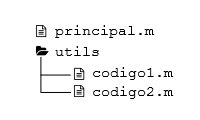
\includegraphics[width=0.3\textwidth]{src/img/ch1/path_example.pdf}
\end{center}

% \begin{verbatim}
% |
% └─── principal.m
% └─── utils
%         └─── codigo1.m
%         └─── codigo2.m
% \end{verbatim}

Una solución evidente (pero muy \emph{tosca}) es colocar los ficheros
\texttt{codigo1.m} y \texttt{codigo2.m} en el mismo directorio, pero
claro, eso implicaría tener muchos ficheros en una misma carpeta, lo
cual no suele ser buena idea.\\

Y la otra solución consiste en agregar la carpeta \texttt{utils} al path
de MATLAB, lo cual es tan sencillo como ejecutar:

\begin{matlab}
>> path(path, 'utils');
\end{matlab}

Con esto podrá llamar los ficheros \texttt{codigo1.m} y
\texttt{codigo2.m} desde \texttt{principal.m} sin necesidad de
colocarlos en la misma carpeta.

\section{Entradas y salidas en el Command Window}\label{entradas-y-salidas-en-el-command-window}

En la sección \ref{descripcion-del-entorno-de-desarrollo} se describió al Command Window (ventana de comandos) y
se hizo referencia a este como la parte del escritorio de MATLAB que
permite interactuar tecleando instrucciones y devolviendo al instante un
resultado. En esta sección veremos cómo utilizar funciones que permitan
introducir y mostrar ciertos valores de manera controlada por el
usuario.

\subsection{La función input}\label{la-funcion-input}

La función input permite \emph{pedir} un valor al usuario utilizando una
cadena de caracteres como prompt, la sintaxis es muy sencilla:

\begin{matlab}
var=input('Introduzca un valor: ');
\end{matlab}

En la variable var se guarda el valor que el usuario introduzca, los
valores aceptados por la función input pueden ser de tipo numérico, cell
arrays, e inclusive tipo char. Aunque para introducir cadenas de texto
la función input dispone de un modificador que hará que la entrada se
evalúe como una variable tipo char o cadena de texto, la sintaxis para
esto es la siguiente:

\begin{matlab}
var=input('Introduzca una cadena de texto: ', 's');
\end{matlab}

La letra s entre comillas simples le indica a MATLAB que deberá evaluar
la entrada como tipo string.

\subsection{Salida sin formato: la función disp}\label{salida-sin-formato-la-funcion-disp}

La función \texttt{disp} muestra en pantalla el valor de una determinada variable
que se pasa como argumento, por ejemplo:

\begin{matlab}
>> a=3;
>> disp(a)
     3
\end{matlab}

Para el caso anterior se pasa como argumento la variable a que ha sido
declarada previamente y simplemente se muestra el valor correspondiente
a esta. Las variables a mostrar pueden ser de cualquier tipo, incluyendo
cadenas de texto, matrices, cell arrays y estructuras, véanse los
siguientes ejemplos:

\begin{matlab}
>> disp(magic(3))
     8     1     6
     3     5     7
     4     9     2
>> disp({1,0,2,-2})
    [1]    [0]    [2]    [-2]
>> disp('Hola Mundo')
Hola Mundo
\end{matlab}

Con disp también es posible mostrar enlaces a un sitio web, utilizando
la sintaxis HTML para un enlace dentro de la función disp, por ejemplo:

\begin{verbatim}
>> disp('<a href="http://matlab-typ.blogspot.mx">MATLAB TYP</a>');
MATLAB TYP
\end{verbatim}

\subsection{La función fprintf}\label{la-funcion-fprintf}

Con \texttt{fprintf} es posible dar formato a la salida que se quiere
imprimir en pantalla, por ejemplo, es posible especificar el número de
decimales que se mostrarán o bien si se quiere mostrar como un entero o
quizá como una cadena de texto. La sintaxis de la función fprintf es
como sigue:

\begin{matlab}
fprintf('Especificaciones de formato',a1,...,an);
\end{matlab}

Donde las especificaciones de formato incluyen uno o más de los
identificadores de un mismo tipo o combinados que se muestran en la
siguiente tabla:

\begin{table}[h!]
\centering
% \rowcolors{1}{}{gray!20}
\begin{tabular}{P{4cm} p{7cm}} 
\hline
\bfseries Identificador & \Centering\bfseries Formato de salida \\
\hline
\texttt{\%d} & Tipo entero \\
\texttt{\%f} & Tipo coma flotante \\
\texttt{\%g} & Tipo coma flotante compacta. \\
\texttt{\%u} & Tipo entero sin signo \\
\texttt{\%e} & Tipo coma flotante, notación exponencial \\
\texttt{\%s} & Tipo char, cadena de texto \\
\texttt{\%c} & Tipo char, carácter a carácter.\\
\hline
\end{tabular}
\caption{Opciones de formato para \texttt{fprintf}}
\end{table}

Véase el siguiente ejemplo:

\begin{matlab}
>> fprintf('%d',pi);
3.141593e+00>>
\end{matlab}

Observe que se imprime el valor de $\pi$ en este caso, pero el
prompt de la ventana de comandos queda situado justo después del valor
de salida en la misma línea, para evitar lo anterior puede utilizar la
secuencia de escape \ver|\n| después del valor a
imprimir, lo cual le indica a MATLAB que debe comenzar en una nueva
línea. Modificamos y vemos el resultado que produce:

\begin{matlab}
>> fprintf('%d\n',pi);
3.141593e+00
\end{matlab}

Ahora observe lo que se imprime utilizando otros identificadores:

\begin{matlab}
>> fprintf('%f\n',pi);
3.141593
>> fprintf('%g\n',pi);
3.14159
>> fprintf('%e\n',pi);
3.141593e+00
>> fprintf('%u\n',pi);
3.141593e+00
\end{matlab}

Para las salidas de coma flotante puede especificar el número de
decimales que tendrá la salida, por ejemplo si desea mostrar solamente
dos decimales del número $\pi$:

\begin{matlab}
>> fprintf('%.2f\n',pi);
3.14
\end{matlab}

\section{Funciones}\label{funciones}

\subsection{Funciones, una introducción}\label{funciones-una-introduccion}

Las funciones son porciones de código que por lo general aceptan
argumentos o valores de entrada y devuelven un valor de salida. Una
función es una herramienta muy útil en la programación, dado que permite
la reutilización de código para procedimientos que lo requieran, así
como una facilidad significativa para mantener el código, lo cual se
traduce en una mayor productividad. MATLAB, de hecho, está compuesto por
una multitud de funciones agrupadas en \emph{toolboxs}, cada una de
ellas pensada para resolver una situación concreta.\\

Una función debe definirse en un fichero único, es decir, por cada
función creada debemos utilizar un archivo \texttt{*.m}, mismo que
tendrá el nombre dado a la función.\\

La estructura básica de una función contiene los siguientes elementos:

\begin{itemize}
\tightlist
\item
  La palabra reservada function
\item
  Los valores de salida
\item
  El nombre de la función
\item
  Los argumentos de entrada
\item
  Cuerpo de la función
\end{itemize}

Para una mejor comprensión de cada uno de esos elementos, refiérase a
las siguientes líneas de código:

\begin{matlab}
function res = suma(a,b)
res = a+b;
end
\end{matlab}

La función anterior llamada \texttt{suma}, recibe como argumentos de
entrada dos valores numéricos a y b, y devuelve un resultado guardado en
res que equivale a la suma aritmética de las variables de entrada. Note
que el valor de retorno debe asignarse a la variable indicada en la
línea de definición.\\

Si ejecutamos la función en la ventana de comandos obtenemos algo
similar a esto:

\begin{matlab}
>> s=suma(3,2)
s =
     5
\end{matlab}

Si no hace una asignación el resultado devuelto se guarda en la variable
\texttt{ans}.

\subsection{Verificar argumentos de entrada y salida}\label{verificar-argumentos-de-entrada-y-salida}

Cuando se crea una función es recomendable verificar si la cantidad de
argumentos de entrada corresponden a los soportados, o bien, si el tipo
de dato que se ha introducido es el adecuado para proceder con el resto
de la programación; MATLAB proporciona los comandos \texttt{nargin} y
\texttt{nargout} que sirven para \emph{contar} el número de argumentos
de entrada y salida respectivamente. \\

Utilizando como ejemplo la función suma creada con anterioridad, podemos
verificar que el número de argumentos sean exactamente dos para poder
proceder y en caso contrario enviar al usuario un mensaje de error en la
ventana de comandos, el código implicado sería similar al siguiente:

\begin{matlab}
function res = suma(a,b)
if nargin==2
    res=a+b;
else
    error('Introduzca dos argumentos de entrada');
end
end
\end{matlab}

Si ejecutamos la función pasándole solamente un argumento de entrada nos
devolverá un mensaje de error:

\begin{matlab}
>> s=suma(7)
Error using suma (line 5)
Introduzca dos argumentos de entrada
\end{matlab}

\subsection{Sub-funciones}\label{sub-funciones}

Las sub-funciones son funciones definidas dentro del espacio de otra
función principal. Se utilizan como funciones auxiliares con la
finalidad de hacer más legible el código y facilitar la depuración de
errores. Enseguida se muestra el ejemplo de una sub-función:

\begin{matlab}
function r=isfibo(num)
% Determina  si un  número  entero  forma  parte
% de la sucesión de Fibonacci, devuelve un valor
% de tipo lógico.
ff=fibonacci(num);
if any(ff==num)
    r=true;
else
    r=false;
end
    function F=fibonacci(n)
        F(1:2)=1;
        i=3;
        while 1
            F=[F F(i-1)+F(i-2)];
            if F(end) >= n,break,end;
            i=i+1;
        end
    end
end
\end{matlab}

La función anterior isfibo determina si el entero pasado como argumento
de entrada pertenece a la sucesión de Fibonacci, para ello utiliza como
una función auxiliar a la sub-función fibonacci que se encarga de
generar la sucesión de Fibonacci en un intervalo dado y guardarlo en un
vector de salida. Una sub-función puede ser llamada solamente por la
función principal que la contiene.

\subsection{Argumentos variables}\label{argumentos-variables}

En la introducción a las funciones se ha mencionado que estas por lo
general tienen un número específico de argumentos de entrada y salida,
no obstante se presentan situaciones en donde los argumentos de entrada
o salida de una función no son fijos o bien los argumentos pueden ser
demasiados de tal modo que resulte incómodo definirlos en la línea
correspondiente. Para solucionar lo anterior MATLAB permite el uso de
\texttt{varargin} y \texttt{varargout} como argumentos de entrada y salida
respectivamente. Para tener una idea más práctica de lo anterior véase
el ejemplo siguiente:

\begin{matlab}
function m=max2(varargin)
if nargin==1
    v=varargin{1};
    m=v(1);
    for i=2:length(v)
        if v(i)>m
            m=v(i);
        end
    end 
elseif nargin==2
    a=varargin{1};
    b=varargin{2};
    if a>b
        m=a;
    else
        m=b;
    end
end
end
\end{matlab}

La función anterior \texttt{max2} emula a la función nativa \texttt{max}, puede recibir
como argumento de entrada un vector o bien dos valores escalares. Si
observa el código anterior notará que varargin es un cell array que
guarda todos los argumentos de entrada pasados a la función, como se
verá en el capítulo 3 la manera de acceder a los elementos de un cell
array es utilizando la sintaxis: \texttt{var\{k\}}, donde \texttt{var}
es la variable en la que está almacenada el cell array y \texttt{k} es
el k-ésimo elemento contenido en el cell array.

\subsection{Ayuda de una función}\label{ayuda-de-una-funcion}

Como parte de las buenas prácticas de programación es recomendable
incluir comentarios dentro de una función que indiquen el propósito de
esta, así como una descripción breve de los argumentos de entrada y
salida e incluso un ejemplo concreto de la misma. \\

Por convención estos comentarios deben colocarse justamente después de
la definición de la función y antes de todo el código restante, además
de que esto servirá como referencia al resto de usuarios también le
permitirá a MATLAB interpretarlo como las líneas de ayuda cuando se le
solicite expresamente mediante la función help. Véase el siguiente
ejemplo:

\begin{matlab}
function [x1,x2]=ecuad(a,b,c)
% Resuelve una ecuación cuadrática de la forma:
% a*x^2+b*x+c=0
%
% Argumentos de entrada:
%          a  -  Coeficiente cuadrático
%          b  -  Coeficiente lineal
%          c  -  Coeficiente constante
%
% Argumentos de salida:
%          x1,x2  - Raíces de la ecuación cuadrática 
%
% Ejemplo:
%         >> [r1,r2]=ecuad(-1,2,1);
%
 
x1=(1/(2*a))*(-b+sqrt(b^2-4*a*c));
x2=(1/(2*a))*(-b-sqrt(b^2-4*a*c));
end
\end{matlab}

Podemos teclear help ecuad en la ventana de comandos y verificar lo que
MATLAB nos devuelve como ayuda de la función:

\begin{matlab}
>> help ecuad
  Resuelve una ecuación cuadrática de la forma:
  a*x^2+b*x+c=0
  Argumentos de entrada:
           a  -  Coeficiente cuadrático
           b  -  Coeficiente lineal
           c  -  Coeficiente constante
  Argumentos de salida:
           x1,x2  - Raíces de la ecuación cuadrática 
  Ejemplo:
          >> [r1,r2]=ecuad(-1,2,1);
\end{matlab}

Es común agregar a la ayuda de una función algunas referencias hacia
otras funciones similares, para ello en los comentarios debe agregar una
línea que comience con las palabras \texttt{SEE ALSO} (Ver también), seguidas
de las funciones similares separadas por comas, véase el ejemplo a
continuación:

\begin{matlab}
function [x1,x2]=ecuad(a,b,c)
% Resuelve una ecuación cuadrática de la forma:
% a*x^2+b*x+c=0
%
% Argumentos de entrada:
%          a  -  Coeficiente cuadrático
%          b  -  Coeficiente lineal
%          c  -  Coeficiente constante
%
% Argumentos de salida:
%          x1,x2  - Raíces de la ecuación cuadrática 
%
% Ejemplo:
%         >> [r1,r2]=ecuad(-1,2,1);
%
% SEE ALSO roots,solve,fzero
%
 
x1=(1/(2*a))*(-b+sqrt(b^2-4*a*c));
x2=(1/(2*a))*(-b-sqrt(b^2-4*a*c));
end

>> help ecuad
  Resuelve una ecuación cuadrática de la forma:
  a*x^2+b*x+c=0 
  Argumentos de entrada:
           a  -  Coeficiente cuadrático
           b  -  Coeficiente lineal
           c  -  Coeficiente constante
  Argumentos de salida:
           x1,x2  - Raíces de la ecuación cuadrática 
  Ejemplo:
          >> [r1,r2]=ecuad(-1,2,1);

  SEE ALSO roots,solve,fzero
\end{matlab}

\section{Bifurcaciones y bucles}

\subsection{Sentencia if-elseif-else}

La sentencia \texttt{if} se utiliza como bifurcación simple por sí sola,
es decir, en aquellas situaciones en las cuales se requiera evaluar
solamente una condición, por ejemplo, suponga que tiene dos números a y
b y necesita comprobar si son iguales y ejecutar una acción, para ello
bastaría con una sentencia \texttt{if} simple:

\begin{matlab}
if a==b
    disp('a es igual a b');
end
\end{matlab}

A diferencia del caso anterior hay situaciones que requieren la
ejecución de una acción cuando la condición se cumpla y de otra en caso
contrario, entonces puede utilizarse una bifurcación doble formada por
las sentencias \texttt{if-else}. Retomando el ejemplo para la
bifurcación \texttt{if} simple, podríamos modificarlo de tal manera que
envíe también un mensaje (ejecute una acción) para cuando la condición
no se cumple:

\begin{matlab}
if a==b
    disp('a es igual a b');
else
    disp('a es diferente de b');
end
\end{matlab}

Ahora imagine que para los ejemplos anteriores se necesita especificar
si a=b, si $a > b$ o bien si $a < b$, lo cual
implicaría tener una sentencia de selección múltiple
\texttt{if-elseif-else} que permite escoger entre varias opciones,
evaluándose en orden descendente, por ejemplo refiérase a la siguiente
estructura:

\begin{matlab}
if cond1
    % Instrucciones
elseif cond2 
    % Instrucciones
elseif cond3
    % Instrucciones
    .
    .
    .
elseif condN
    % Instrucciones
else
    % Instrucciones
end
\end{matlab}

MATLAB evalúa primeramente la condición 1 contenida en la sentencia
\texttt{if} (cond1) y en el caso de no cumplirse evalúa la siguiente
condición de forma sucesiva (cond2, cond3, ...); finalmente y en el
caso de que ninguna de las opciones evaluadas se cumpla, se ejecuta la
instrucción contenida en la sentencia else. A continuación se muestra el
ejemplo de una bifurcación múltiple para la situación descrita al
principio:

\begin{matlab}
if a==b
    disp('a es igual que b');
elseif a>b
    disp('a es mayor que b');
elseif a<b
    disp('a es menor que b');
end
\end{matlab}

\subsection{Sentencia switch}\label{sentencia-switch}

La sentencia switch es una bifurcación múltiple que permite seleccionar
entre varias opciones o casos la acción a ejecutar. La sintaxis general
es:

\begin{matlab}
switch var
   case opc1
      % Instrucciones
   case opc2
      % Instrucciones
    .
    .
    .
   otherwise
      % Intrucciones
end
\end{matlab}

Siendo var la variable que servirá como criterio de selección. Después
de la palabra reservada case, se coloca el valor de var para el cual se
ejecutarán esas instrucciones, y en otherwise se insertan las
instrucciones que MATLAB deberá ejecutar por defecto en caso de no
cumplirse ninguno de los casos especificados. \\

Enseguida se muestran dos ejemplos correspondientes a la sentencia de
selección switch:

\begin{matlab}
X=input('Inserte 0 o 1: ');
switch X
    case 0
        disp('Insertó cero');
    case 1
        disp('Insertó uno');
    otherwise
        warning('Valor incorrecto, verifique');     
end


letra=input('Inserte una letra: ','s');
switch letra
    case {'a','e','i','o','u'}
        disp('Es una vocal');
    otherwise
        disp('Es una consonante');
end
\end{matlab}

\subsection{Bucle for}\label{bucle-for}

La sintaxis general de un bucle for se muestra enseguida:

\begin{matlab}
for i=inicio:incremento:fin
    % Instrucciones...
end
\end{matlab}

El valor inicio es a partir del cual se ejecutará el ciclo, el
incremento es la cantidad que varía en cada paso de ejecución, y el
valor de final establece el último valor que tomará el ciclo.\\

El siguiente código muestra un ciclo for muy básico, el cual simplemente
muestra en consola el valor actual adquirido por la variable.

\begin{matlab}
for i=1:10
    fprintf('Valor actual: %g \n',i);
end
\end{matlab}

Cuando no se especifica el incremento, como el caso anterior, MATLAB
asume que es unitario.\\

Es posible utilizar ciclos for anidados, por ejemplo para cuando se
requiere recorrer una matriz en sus dos dimensiones y ejecutar
operaciones elemento por elemento. Véase el siguiente ejemplo:

\begin{matlab}
A=round(rand(5)*10);
for i=1:5
    for j=1:5
        disp(A(i,j));
    end
end
\end{matlab}

\subsection{Bucle while}\label{bucle-while}

El bucle while se utiliza, por lo general, cuando no se tiene un rango
definido sobre el cual se realice la ejecución del ciclo o bien cuando
la terminación del mismo viene dada por una condición. La sintaxis más
común es:

\begin{matlab}
while cond
    % Instrucciones
    % ...
    % ...
    % ...
end
\end{matlab}

Donde \texttt{cond} es la condición que determina la finalización de
ejecución. \\

Enseguida se muestra un ejemplo muy básico que muestra en pantalla el
valor de una variable utilizada como referencia:

\begin{matlab}
k=1;
while k<10
    disp(k);
    k=k+1;
end
\end{matlab}

Lo anterior muestra en consola el valor de k mientras esta sea menor a
10, es decir muestra todos los valores enteros en el intervalo
$[1,9]$, es importante notar que la variable k debe
incrementarse en cada ciclo para que en un momento determinado la
condición de finalización se cumpla, de lo contrario se convertiría en
un bucle infinito. \\

Ahora, veamos un ejemplo más práctico. La aproximación de una raíz
cuadrada por el método babilónico implica realizar n iteraciones
mediante la siguiente expresión:

$$ r_n(x) = \frac{1}{2} \left( \frac{x}{r_{n-1}}+r_{n-1} \right) $$

Donde x es el número del cual se calcula la raíz cuadrada. A
continuación se muestra el código implementado en MATLAB utilizando un
bucle \texttt{while}:

\begin{matlab}
x=input('Introduzca un número positivo: ');
r=x;
ra=0;
while ra~=r
    ra=r;
    r=(1/2)*(x/r+r);
end
fprintf('\nRaíz cuadrada de %g = %g\n\n',x,r);
\end{matlab}

Como se observa, en la variable ra se guarda la raíz aproximada
calculada en una iteración anterior, de manera que esta sirva como
comparación respecto a la nueva raíz calculada, el bucle termina cuando
la diferencia entre el valor actual y el anterior es inferior a la
tolerancia numérica (\texttt{eps}) soportada por MATLAB y por ende pasan
a considerarse como valores iguales. \\

\begin{informacion}{While-if-break, rompiendo ciclos.}
Es común utilizar el ciclo while poniendo un valor verdadero como condición, y 
usar la sentencia combinada \texttt{if-break} como punto de parada, por ejemplo:

\begin{matlab}
while true
    a = randi(10);
    if a>5
        break;
    end
end
\end{matlab}
\end{informacion}

\section{Fecha y hora}

Primeramente es importante mencionar que MATLAB maneja tres formatos de
fechas y hora, a saber:

\begin{itemize}
\item
  Un vector de seis elementos los cuales son: {[}año, mes, día, hora,
  minuto, segundo{]}.
\item
  Un valor escalar de coma flotante (tipo double), en el cual la parte
  entera representa la cantidad de días que han transcurrido desde el
  año cero (calendario gregoriano) y la parte decimal representa la
  fracción del día trascurrido.
\item
  Una cadena de texto con la forma \texttt{’dd-mmm-aaa\ HH:MM:SS’}.
\end{itemize}

Para obtener la fecha actual MATLAB proporciona el comando now:

\begin{matlab}
>> now
ans =
   7.3575e+05
\end{matlab}

Lo anterior podría resultar útil para efectos de cálculo pero no es tan
significativo para el usuario que está acostumbrado a visualizar la
fecha y hora mediante los formatos convencionales; podemos convertir el
valor numérico anterior a una cadena de texto que nos proporcione mayor
información a primer vista, para ello se utiliza la función datestr como
sigue:

\begin{matlab}
>> datestr(now)
ans =
03-Jun-2014 17:09:36
\end{matlab}

Además de las anteriores MATLAB dispone de las funciones datevec y
clock, la primera convierte una determinada fecha pasada como argumento
en formato string o numérico a un vector de seis elementos como se
describió anteriormente, y clock devuelve la fecha y hora actual tal
como la hace \texttt{now} pero como un vector de seis elementos. \\


\begin{ejemplo}{Ejemplo 1.1 Calculando área y perímetro de un círculo}
El área y perímetro (circunferencia) de un círculo vienen dados por las 
siguientes ecuaciones:

$$ A = \pi r^2 $$
$$ P = 2 \pi r $$

Escriba un programa que reciba como dato de entrada el radio del 
círculo y que imprima en consola el área y perímetro. \\

\textbf{Solución} \\

\begin{matlab}
r = input('Radio: ');
A = pi*r.^2;
P = 2*pi.*r;
fprintf('\nÁrea: %0.4f \nPerímetro: %0.4f \n\n',A,P);
\end{matlab}

Si ejecutamos el programa obtendremos algo como lo siguiente:

\begin{verbatim}
Radio: 5

Área: 78.5398 
Perímetro: 31.4159 
\end{verbatim}

\end{ejemplo} 

  \\  

\begin{ejemplo}{Ejemplo 1.2 Clasificando flujos}

El número de Reynolds es un parámetro adimensional utilizado en
mecánica de fluidos para caracterizar el movimiento de un fluido,
usualmente para un flujo interno en tuberías circulares se define como:

$$ Re=\frac{vD}{\nu} $$

Donde v es la velocidad del fluido, D el diámetro de la tubería a
través de la cual circula el fluido y $\nu$ la viscosidad cinemática.
La teoría subyacente del número de Reynolds se establece conforme a
varias características propias y externas al fluido, pero en este caso
vamos a limitarlo al flujo interno en tuberías circulares; siendo así,
el número de Reynolds permite caracterizar si un flujo es laminar o
turbulento dependiendo de ciertos intervalos establecidos de manera
experimental, enseguida se muestran los intervalos de valores y el
tipo de flujo en cada caso:

\begin{itemize}
\item Re $<$ 2100  \textit{Flujo laminar}
\item 2100 $\leq$ Re $\leq$ 3000   \textit{Flujo transitorio}
\item Re $>$ 3000   \textit{Flujo turbulento}
\end{itemize}

Basado en lo anterior, escriba un programa cuyos valores de entrada
sean la velocidad del fluido, el diámetro de la tubería y la
viscosidad cinemática, y que devuelva como variable de salida el tipo
de flujo.\\

\textbf{Solución:}

Vamos a implementar una solución utilizando la estructura de control 
\texttt{if-elseif-else}, en la cual nuestra variable o dato de comprobación 
será el número Reynolds.

\begin{matlab}
velocidad = input('Velocidad: ');
diametro = input('Diámetro: ');
viscosidad = input('Viscosidad: ');

Re = (velocidad*diametro)/(viscosidad);

if Re<2100
   disp('Flujo laminar');
elseif Re >= 2100 && Re <= 3000
   disp('Flujo transitorio');
else
   disp('Flujo turbulento');
end
\end{matlab}

¿Parece lo anterior una buena solución?.\\

Está muy bien, pero, y si alguien tiene la brillante idea de colocar 
cantidades negativas; el programa nunca se "quejará", pero desde luego estaremos 
entrando en una situación un tanto extraña, seguramente el programa nos mandará que 
estamos en el caso de un flujo turbulento, aún cuando los datos ingresados sean incorrectos.
Luego, lo que se quiere mostrar es que necesitamos trabajar más aún sobre ese código, 
asegurarnos que los datos ingresados sean los adecuados para realizar el cálculo. 
Claro está que en un código que necesitemos para nuestros deberes académicos pueda 
sonar un poco absurdo, pero en el mundo real estas cosas nunca, nunca están de más.
\end{ejemplo}

\section*{Problemas}

\textbf{1.1} ¿Qué tipo de dato devuelve cada una de las siguientes
instrucciones? (Puede verificar utilizando la función \texttt{class}).

\begin{matlab}
>> 3;
>> true;
>> 3==2;
>> {1,2,3}; 
\end{matlab}

\textbf{1.2} ¿Es posible realizar las siguientes operaciones?

\begin{matlab}
>> 3+int8(2);
>> true+5;
>> int8(10)+int16(5);
>> {1,2,3}+{0,1,0};
>> [5,1,-2]+[2 3 0];
\end{matlab}

\textbf{1.3} Desarrolle un script que le solicite su nombre (utilice la
función input) y que devuelva un saludo más el nombre ingresado, por
ejemplo: Hola Jorge, bienvenido. \\

\textbf{1.4} Identifique el error en las siguientes líneas de código:

\begin{matlab}
edad=input('Introduzca su edad: ','s');
if edad >= 18
    disp('Mayor de edad');
else
    disp('Menor de edad');
end
\end{matlab}

\textbf{1.5} Utilizando la escala de calificación del 0 a 10 y siendo 6
la calificación mínima aprobatoria, cree un programa en el cual ingrese
una calificación y este le devuelva un mensaje de APROBADO o NO APROBADO
en el caso que corresponda. \\

\textbf{1.6} El siguiente es un problema clásico en los cursos básicos
de programación: escriba un programa que determine si un número
ingresado es par o impar. \\

\textbf{1.7} Escriba una función llamada \texttt{sfibonacci}, que reciba
como argumento un entero positivo n, y que devuelva un vector con los
primeros n términos de la sucesión de Fibonacci. \\

\textbf{1.8} Desarrolle una función llamada \texttt{bucle\_test}, que
reciba como argumento de entrada un número entero N. Esta función debe
recorrer todos los valores enteros en el rango de 1 a N mostrando ``n es
divisible por 2'', ``n es divisible por 3'', ``n es divisible por 2 y
3'' o ``n no es divisible por 2 o 3'' (donde n será el valor actual).
Use un bucle for para recorrer los valores, la función \texttt{rem} para
verificar la divisibilidad y \texttt{num2str} para convertir cada número
en un string y mostrarlo en pantalla. Para verificar cada caso puede
utilizar una bifurcación múltiple \texttt{if-elseif-else}. 
\footnote{Danilo
  Šćepanović. 6.094 Introduction to MATLAB, January IAP 2010.
  (Massachusetts Institute of Technology: MIT OpenCourseWare),
  http://ocw.mit.edu (Accessed).} \\

\textbf{1.9} Escriba una función que le permita determinar si un número
entero pasado como argumento es primo, en caso de serlo devolverá un
valor lógico true y un valor false en caso contrario. (La función
\texttt{isprime} de MATLAB realiza la misma operación, pero claro, evite utilizarla 
en este caso).

% \chapter{Vectores y matrices}

\section{Creando matrices y vectores}

Una matriz es un arreglo bidimensional de elementos, que para efectos de
este capítulo serán siempre, a menos que se especifique lo contrario, de
tipo numérico. Cada elemento de una matriz se identifica por la posición
(número de fila y columna) que ocupa. De forma generalizada y siendo m
el subíndice correspondiente a una fila y n el de columna, una matriz se
representa como sigue:

$$
A_{m,n} = 
\begin{pmatrix}
a_{1,1} & a_{1,2} & \cdots & a_{1,n} \\
a_{2,1} & a_{2,2} & \cdots & a_{2,n} \\
\vdots  & \vdots  & \ddots & \vdots  \\
a_{m,1} & a_{m,2} & \cdots & a_{m,n} 
\end{pmatrix}
$$

Un vector es un caso particular de matriz que sólo contiene una fila o
una columna.

\subsection{Insertando valores
manuales}\label{insertando-valores-manuales}

Crear una matriz en MATLAB es muy sencillo, dado que la sintaxis es muy
simple. Se escriben entre corchetes todos los valores pertenecientes a
la matriz, separándose por comas o espacios elementos de una misma fila
y diferente columna, y por punto y coma aquellos que correspondan a otra
fila.

\textbf{Ejemplo}. Defina la matriz \textbf{A} utilizando MATLAB

$$
A = 
\begin{pmatrix}
    -1 & 2 & 1 \\
    0 & 7 & -3 \\
    1 & -1 & -2
\end{pmatrix}
$$

Enseguida se muestran dos formas equivalentes realizar lo que se pide:

\begin{matlab}
>> A=[-1 2 1;0 7 -3;1 -1 -2]
A =
    -1     2     1
     0     7    -3
     1    -1    -2
>> A=[-1,2,1;0,7,-3;1,-1,-2]
A =
    -1     2     1
     0     7    -3
     1    -1    -2
\end{matlab}

Como se observa, es indistinto colocar espacios o comas para separar
valores de una misma fila.

\subsection{Generar matrices y vectores predefinidos}\label{generar-matrices-y-vectores-predefinidos}

\subsubsection{Matriz de ceros}\label{matriz-de-ceros}

MATLAB dispone de la función zeros, que crea una matriz con las
dimensiones pasadas como argumento; puede además especificarse la clase
o tipo de dato. Por ejemplo si tecleamos la siguiente instrucción:

\begin{matlab}
>> M=zeros(5)
M =
     0     0     0     0     0
     0     0     0     0     0
     0     0     0     0     0
     0     0     0     0     0
     0     0     0     0     0
\end{matlab}

Se crea una matriz cuadrada de 5x5 rellena de ceros de la clase double.
Si pasamos dos argumentos numéricos al llamar la función, estos
corresponderán al número de filas y columnas respectivamente, véase el
siguiente ejemplo de una matriz de 3x2:

\begin{matlab}
>> M=zeros(3,2)
M =
     0     0
     0     0
     0     0
\end{matlab}

En caso de que necesite que los elementos de la matriz de ceros sean de
una clase distinta a double, puede incluir la opción del tipo de dato
como argumento, tal como se muestra en el siguiente ejemplo:

\begin{matlab}
>> M=zeros(3,4,'uint8')
M =
    0    0    0    0
    0    0    0    0
    0    0    0    0
>> whos
  Name      Size            Bytes  Class    Attributes
  M         3x4                12  uint8              
\end{matlab}

\subsubsection{Matriz de unos}\label{matriz-de-unos}

Para crear una matriz cuyos elementos sean todos unos MATLAB cuenta con
la función \texttt{ones}, la sintaxis es prácticamente la misma que para
la función \texttt{zeros}, véanse los ejemplos siguientes:

\begin{matlab}
>> A=ones(3)
A =
     1     1     1
     1     1     1
     1     1     1
>> A=ones(5,2,'uint8')
A =
    1    1
    1    1
    1    1
    1    1
    1    1
>> whos
  Name      Size            Bytes  Class    Attributes
  A         5x2                10  uint8      
\end{matlab}

\subsubsection{Matriz identidad}\label{matriz-identidad}

Para crear una matriz identidad MATLAB proporciona la función
\texttt{eye}, recuerde que una matriz identidad es aquella que contiene
unos en la diagonal principal y ceros en el resto de elementos. Se
muestra a continuación una matriz identidad de 3x3:

\begin{matlab}
>> I=eye(3)
I =
     1     0     0
     0     1     0
     0     0     1
\end{matlab}

\subsubsection{La función linspace}\label{la-funcion-linspace}

La función linspace genera un vector de elementos equiespaciados o de
escala lineal. Los argumentos de entrada son los límites del intervalo:

\begin{matlab}
>> linspace(a,b)
\end{matlab}

La línea anterior genera un vector de 100 elementos linealmente
distribuidos entre los valores a y b, si necesita más o menos elementos
puede especificar la cantidad como un tercer argumento, véanse los
siguientes ejemplos:

\begin{matlab}
>> linspace(0,10,5)
ans =
         0    2.5000    5.0000    7.5000   10.0000
>> linspace(-2,2,5)
ans =
    -2    -1     0     1     2
\end{matlab}

\subsection{Generar vectores con el operador dos puntos}\label{generar-vectores-con-el-operador-dos-puntos}

El operador dos puntos es quizá el más utilizado en la programación en
MATLAB, todo aquello que involucre matrices o vectores lleva consigo el
uso de este operador. Por ahora simplemente veremos cómo crear vectores
con este operador en un intervalo, en secciones posteriores se verá el
uso de este operador en el indexado de matrices.\\

Crear un vector con este operador resulta en una sintaxis muy sencilla,
en el caso más básico solo hay que especificar los límites del vector
separados por los dos puntos, es decir:

\begin{matlab}
>> a:b 
\end{matlab}

La instrucción anterior genera la secuencia , la siguiente línea con un
caso concreto ejemplifica de una mejor manera:

\begin{matlab}
>> 1:10
ans =
     1     2     3     4     5     6     7     8     9    10
\end{matlab}

Si requiere especificar el \emph{paso} o incremento de los elementos que
conformarán la secuencia puede hacerse mediante la sintaxis:

\begin{matlab}
>> a:paso:b 
\end{matlab}

Por ejemplo:

\begin{matlab}
>> 0:2:10
ans =
     0     2     4     6     8    10
>> 0:0.2:1
ans =
         0    0.2000    0.4000    0.6000    0.8000    1.0000
\end{matlab}

Desde luego que puede generarse un vector utilizando el orden inverso,
es decir, con valores en forma descendente, revise el siguiente ejemplo:

\begin{matlab}
>> 100:-10:0
ans =
   100    90    80    70    60    50    40    30    20    10     0
\end{matlab}

\subsection{Matrices de números aleatorios}\label{matrices-de-numeros-aleatorios}

Con la función \texttt{rand} MATLAB genera arreglos de números
aleatorios con valores entre 0 y 1, la sintaxis de \texttt{rand} es:

\begin{matlab}
M = rand(nf, nc);
\end{matlab}

Donde nf es el número de filas y nc el número de columnas, si la matriz
es cuadrada puede especificarse sólo un valor como argumento de entrada.
Compute y verifique en MATLAB los siguientes ejemplos:

\begin{matlab}
>> R=rand(5)
R =
    0.3439    0.6618    0.0523    0.5728    0.3251
    0.1229    0.1329    0.2557    0.6078    0.7994
    0.4799    0.2256    0.4457    0.5250    0.7819
    0.4365    0.1340    0.2022    0.6430    0.6300
    0.6780    0.5367    0.8866    0.2912    0.4490
>> M=rand(4,3)
M =
    0.3814    0.2016    0.6681
    0.2810    0.4626    0.4703
    0.5331    0.1055    0.1873
    0.6376    0.3538    0.0297
\end{matlab}

Una matriz de números aleatorios enteros en un rango personalizado,
incluyendo números negativos, puede generarse con la función randi, cuya
sintaxis es:

\begin{matlab}
randi([imin imax], [nf nc]);
\end{matlab}

Siendo imin el valor mínimo del intervalo e imax el valor máximo, nf el
número de filas y nc el número de columnas de la matriz.

\begin{matlab}
>> A=randi([-10 10],[7 6])
A =
     8     7     4    -6    -9     3
    -8    -2     7     4    -1    -9
     9    -4    -5   -10     2    -4
     7     8    -9     7    10     2
    -1     8     2    -6     4    -2
    -6     7   -10     6    -2     9
    -5   -10     1    -6    -9    10
\end{matlab}

\section{Operaciones básicas con matrices}\label{operaciones-basicas-con-matrices}

\subsection{Suma y resta}\label{suma-y-resta}

La suma y resta de matrices está definida para aquellas con las mismas
dimensiones dado que son operaciones que se realizan elemento a
elemento. Si se tienen dos matrices \textbf{A} y \textbf{B} de 3x3
definidas como sigue:

$$
\textbf{A}=
\begin{pmatrix}
    a_{11} & a_{12} & a_{13} \\
    a_{21} & a_{22} & a_{23} \\
    a_{31} & a_{32} & a_{33}
\end{pmatrix}
\,\,\,\,
\textbf{B}=
\begin{pmatrix}
    b_{11} & b_{12} & b_{13} \\
    b_{21} & b_{22} & b_{23} \\
    b_{31} & b_{32} & b_{33}
\end{pmatrix}
$$

La suma viene dada por:

$$
\textbf{A+B} = \begin{pmatrix}
    a_{11}+b_{11} & a_{12}+b_{12} & a_{13}+b_{13} \\
    a_{21}+b_{21} & a_{22}+b_{22} & a_{23}+b_{23} \\
    a_{31}+b_{31} & a_{32}+b_{32} & a_{33}+b_{33}
\end{pmatrix}
$$

En MATLAB sumar y restar matrices o vectores resulta muy sencillo, véase
el ejemplo siguiente:

\begin{matlab}
>> A=[-1 0 3;0 2 1;7 5 1]
A =
    -1     0     3
     0     2     1
     7     5     1
>> B=[1 3 4;2 2 -3;-2 0 1]
B =
     1     3     4
     2     2    -3
    -2     0     1
>> A+B
ans =
     0     3     7
     2     4    -2
     5     5     2
>> A-B
ans =
    -2    -3    -1
    -2     0     4
     9     5     0
>> B-A
ans =
     2     3     1
     2     0    -4
    -9    -5     0
\end{matlab}

\subsection{Multiplicación}\label{multiplicacion}

Para efectuar la multiplicación de matrices es necesario que estas
cumplan algunas características. Suponga que se tienen dos matrices
\textbf{A} y \textbf{B}, y quiere calcular el producto matricial
$A \ast B$, entonces la matriz \textbf{A} debe tener tantas columnas
como número de filas tenga \textbf{B} . En términos más amables: si
\textbf{A} es una matriz de dimensiones mxn entonces la matriz \textbf{B} debe
ser de dimensión nxp, siendo, m,n y p enteros positivos cualesquiera.\\

Para ejemplificar como ejecutar la multiplicación de matrices en MATLAB
crearemos dos matrices \textbf{A} y \textbf{B} de forma aleatoria:

\begin{matlab}
>> A=round(rand(3,5)*5)
A =
     5     4     0     3     4
     3     4     5     1     1
     2     3     0     2     4
>> B=round(rand(5,6)*5)
B =
     4     0     2     0     2     3
     2     3     1     3     4     0
     1     3     4     1     3     4
     1     4     4     3     4     3
     4     5     2     2     1     5
>> C=A*B
C =
    47    44    34    29    42    44
    30    36    36    22    42    37
    32    37    23    23    28    32
\end{matlab}

Si se intenta realizar la multiplicación $B \ast A$, MATLAB devolverá
un error dado que el número de columnas de \textbf{B} (6) es diferente
de la cantidad de filas de \textbf{A} (3).

\begin{matlab}
>> C=B*A
Error using  * 
Inner matrix dimensions must agree. 
\end{matlab}

\section{Operaciones elemento a elemento}\label{operaciones-elemento-a-elemento}

Las operaciones elemento a elemento se ejecutan entre vectores o
matrices cuyas dimensiones son las mismas, cierto es que en muchos casos
este tipo de operaciones no tienen un equivalente matemático definido,
pero son muy útiles para operar con múltiples elementos y aprovechar los
beneficios de la vectorización. Por defecto la suma y resta de arreglos
matriciales se ejecutan, como es de esperarse, elemento a elemento, no
así multiplicación que normalmente está definida bajo los principios
básicos del álgebra lineal.\\

Para forzar a que una multiplicación se haga elemento a elemento debe
utilizarse el operador de multiplicación antecedida por un punto, por
ejemplo:

\begin{matlab}
>> U=[0 -2 1 3 4]
U =
     0    -2     1     3     4
>> V=[-1 3 2 2 7]
V =
    -1     3     2     2     7
>> U.*V
ans =
     0    -6     2     6    28
\end{matlab}

Es sabido que matemáticamente la multiplicación no está definida para
vectores, pero como puede observar en el ejemplo anterior cada elemento
de U ubicado en la k-ésima posición se multiplica por el elemento de V
ubicado en la correspondiente posición. \\

Lo mismo sucede para el caso de la división, formalmente no existe en el
cálculo matricial, pero si está definida en MATLAB como una operación
elemento a elemento, véase el ejemplo siguiente:

\begin{matlab}
>> A=ones(3)
A =
     1     1     1
     1     1     1
     1     1     1
>> B=reshape(1:9,3,3)
B =
     1     4     7
     2     5     8
     3     6     9
>> format rat;
>> A./B
ans =
       1              1/4            1/7     
       1/2            1/5            1/8     
       1/3            1/6            1/9    
 
\end{matlab}

Como se observa, cada elemento de la matriz A es dividido por el
correspondiente en B. Si la instrucción reshape le parece extraña no se
preocupe, en secciones posteriores se verá muy detalladamente. La
instrucción format rat permite visualizar de forma racional las salidas
en la ventana de comandos.

\section{Acceder a elementos de una matriz}\label{acceder-a-elementos-de-una-matriz}

Los elementos de una matriz se identifican mediante la posición que
ocupan en esta, es decir la fila y columna a la cual pertenecen. En
muchos casos se hace necesario operar sobre un elemento específico de
una matriz, y ello implica acceder a este de forma individual, en MATLAB
se puede utilizar la sintaxis siguiente:

\begin{matlab}
>> A(i,j);
\end{matlab}

Con lo anterior se obtiene el elemento perteneciente a la matriz A,
ubicado en la i-ésima fila y j-ésima columna, evidentemente i y j son
enteros positivos cualesquiera, sin exceder, claro, las dimensiones de
la matriz en cuestión. Por ejemplo:

\begin{matlab}
>> A=magic(3)
A =
     8     1     6
     3     5     7
     4     9     2
>> A(1,2)
ans =
     1
\end{matlab}

Para el ejemplo mostrado es evidente que el elemento ubicado en la
primera fila y segunda columna es justamente la unidad. \\

En ocasiones se hace necesario obtener todos o algunos de los elementos
de una fila o columna de una matriz (operación conocida como
\emph{slicing}), para tal efecto se hace uso del operador dos puntos ( :) 
tal como se muestra en el ejemplo siguiente:

\begin{matlab}
>> A=randi(10,3)
A =
     7     1     8
     4     5     8
    10     4     2
>> A(:,1)
ans =
     7
     4
    10
>> A(1,:)
ans =
     7     1     8
\end{matlab}

Note que el colocar dos puntos en la posición de filas o columnas hace
que MATLAB no devuelva una posición única, si no todas las filas o
columnas correspondientes.

\section{Tamaño de las matrices y vectores}\label{tamanio-de-las-matrices-y-vectores}

Determinar el número de filas o columnas de una matriz o bien el número
de elementos que le componen, puede resultar muy útil en situaciones en
las que necesite por ejemplo recorrer con bucles una matriz o bien
acceder sus elementos evitando exceder las dimensiones de la misma. \\

La función size devuelve el número de filas y columnas con la sintaxis:

\begin{matlab}
[m,n]=size(A);
\end{matlab}

Donde A es la matriz, m es el número de filas y n el número de columnas.

Ejemplo:

\begin{matlab}
>> A=ones(5,6)
A =
     1     1     1     1     1     1
     1     1     1     1     1     1
     1     1     1     1     1     1
     1     1     1     1     1     1
     1     1     1     1     1     1
>> [m,n]=size(A)
m =
     5
n =
     6
\end{matlab}

La función size también puede utilizarse con la sintaxis siguiente:

\begin{matlab}
a=size(A,k);
\end{matlab}

Donde k puede adquirir valores de 1 o 2, siendo k=1 se puede determinar
el número de filas y con k=2 se calcula el número de columnas.

\section{Concatenar, rotar y redimensionar una matriz}\label{concatenar-rotar-y-redimensionar-una-matriz}

\subsection{Concatenación de matrices}\label{concatenacion-de-matrices}

La concatenación de matrices es en términos prácticos la unión de dos o
más matrices en una nueva, sin afectar la distribución original de los
elementos. Observe el siguiente ejemplo:

\begin{matlab}
>> M=[ones(3) zeros(3)]
M =
     1     1     1     0     0     0
     1     1     1     0     0     0
     1     1     1     0     0     0
\end{matlab}

La matriz M resulta de la concatenación de dos matrices de ceros y unos
de 3x3 de forma horizontal. Para la concatenación de forma vertical debe
separar cada matriz utilizando el operador punto y coma, como se muestra
a continuación:

\begin{matlab}
>> M=[ones(3);zeros(3)]
M =
     1     1     1
     1     1     1
     1     1     1
     0     0     0
     0     0     0
     0     0     0
\end{matlab}

Si quiere evitar el uso de operadores puede recurrir a las funciones
horzcat y vertcat de MATLAB que prácticamente devuelven resultados
similares a los anteriores. Puede verificar lo anterior con las
instrucciones siguientes:

\begin{matlab}
>> M=horzcat(ones(3),zeros(3));
>> M=vertcat(ones(3),zeros(3));
\end{matlab}

Más aun, MATLAB proporciona la función cat para realizar concatenaciones
en cualquiera de las dimensiones de una matriz. La sintaxis es:

\begin{matlab}
cat(dim,A,B);
\end{matlab}

Donde dim es la dimensión en la cual se concatenarán las matrices A y B,
siendo 1 para las filas (equivalente a vertcat), 2 para las columnas
(equivalente a horzcat) y 3 para la concatenación en una hipermatriz.\\

Considere las matrices \textbf{M} y \textbf{N} definidas como:


$$
\textbf{M}=
\begin{pmatrix}
    1 & 3 \\
    -2 & 1 
\end{pmatrix}
\,\,\,\,
\textbf{N}=
\begin{pmatrix}
    3 & 7 \\
    0 & 2
\end{pmatrix}
$$

Observe los resultados que se producen utilizando la función
\texttt{cat} para cada una de las dimensiones:

\begin{matlab}
>> C=cat(1,M,N)
C =
     1     3
    -2     1
     3     7
     0     2
>> C=cat(2,M,N)
C =
     1     3     3     7
    -2     1     0     2
>> C=cat(3,M,N)
C(:,:,1) =
     1     3
    -2     1
C(:,:,2) =
     3     7
     0     2
\end{matlab}

\subsection{Rotación de matrices}\label{rotacion-de-matrices}

La rotación de matrices consiste en redefinir la posición de sus
elementos mediante una modificación que no afecta el valor de sus
elementos. Para comenzar, suponga que se tiene un vector v definido como
sigue:

$$v = [ v_1 , v_2 , v_3, \cdots , v_{n-1} ,v_n ]$$

Y sea vea v' el vector cuyas componentes son las mismas que v pero
dispuestas en un orden inverso, es decir:

$$v\prime = [v_n , v_{n-1} ,\cdots , v_3 ,v_2 ,v_1 ]$$

En MATLAB invertir el orden de los elementos de un vector resulta una
tarea muy sencilla, esto puede lograrse indexando los elementos de la
forma que a continuación se muestra:

\begin{matlab}
>> v=[-2 5 8 7 3 0] % Vector original
v =
    -2     5     8     7     3     0
>> vp=v(end:-1:1) % Vector con elementos invertidos
vp =
     0     3     7     8     5    -2
\end{matlab}

La anterior es una forma muy simple de realizar dicha tarea, pero si
usted prefiere el uso de funciones existe para tal fin la función fliplr
cuya tarea es exactamente esa, extendiéndose su uso también a matrices,
véase el ejemplo utilizando el mismo vector definido anteriormente:

\begin{matlab}
>> vp=fliplr(v)
vp =
     0     3     7     8     5    -2
\end{matlab}

La función fliplr rota una matriz en un eje vertical, de tal modo que
las columnas situadas a la izquierda queden en la parte derecha. Véase
el ejemplo a continuación:

\begin{matlab}
>> A=randi(10,3)
A =
     4     5     3
     2     2     4
     5     6     6
>> Ar=fliplr(A)
Ar =
     3     5     4
     4     2     2
     6     6     5
\end{matlab}

Está claro que fliplr ejecuta una rotación basada en las columnas, pero
MATLAB dispone también de la función flipud que ejerce una rotación en
un eje horizontal o basada en las filas, enseguida se muestra un
ejemplo:

\begin{matlab}
>> A=randi(10,4)
A =
     5     6     8     2
     9     4     5     3
     8     2     1     5
    10     7     3     6
>> Ar=flipud(A)
Ar =
    10     7     3     6
     8     2     1     5
     9     4     5     3
     5     6     8     2
\end{matlab}

Además de las anteriores MATLAB proporciona la función rot90 que permite
girar la matriz en un ángulo múltiplo de 90° en el sentido contrario a
las manecillas del reloj, de manera informal es como si la matriz rodase
en dirección izquierda. Los argumentos de entrada de la función son
primeramente la matriz a rotar y como segundo argumento un escalar
entero que indica el múltiplo de 90° con el cual habrá de ejecutarse la
rotación, si no se introduce un segundo argumento se asume que este será
unitario. Véanse los ejemplos a continuación:

\begin{matlab}
>> A=randi(20,3)
A =
    14     8    10
     1    19     9
    13     1    10
>> A90=rot90(A)  % Matriz rotada 90°
A90 =
    10     9    10
     8    19     1
    14     1    13
>> A180=rot90(A,2)  % Matriz  rotada en 180°
A180 =
    10     1    13
     9    19     1
    10     8    14
>> A270=rot90(A,3)   % Matriz rotada 270°

A270 =

    13     1    14
     1    19     8
    10     9    10
\end{matlab}

\subsection{Redimensionar matrices}\label{redimensionar-matrices}

Para efectos de esta sección, entiéndase redimensionar como la acción de
transformar la disposición de los elementos de una matriz sin afectar
sus valores ni el número total de elementos, pero si sus posiciones y/o
número de filas o columnas. Por ejemplo, sea A una matriz de m x n, y
sea B una matriz de p x q resultante de redimensionar la matriz A, es
entonces estrictamente necesario que se cumpla la condición
(m)(n)=(p)(q) para que estemos tratando con un \emph{redimensionamiento}. \\

MATLAB cuenta con la función \texttt{reshape} para el redimensionamiento
de matrices, la sintaxis es:

\begin{matlab}
>> X=reshape(A, m, n);
\end{matlab}

Siendo A la matriz original de dimensiones diferentes de m x n (o al
menos eso se espera), m y n son el número de filas y columnas,
respectivamente, que tendrá la nueva matriz X. Véanse los ejemplos
siguientes:

\begin{matlab}
>> V=1:10;
>> X=reshape(V,5,2)
X =
     1     6
     2     7
     3     8
     4     9
     5    10
>> Y=reshape(ones(4),2,8)
Y =
     1     1     1     1     1     1     1     1
     1     1     1     1     1     1     1     1
\end{matlab}

\section{Ordenar matrices}\label{ordenar-matrices}

El ordenamiento de datos es una tarea muy común dentro del mundo de la
informática y en la programación científica. Se ordenan datos para
realizar análisis cualitativos, para la visualización gráfica o
cualquier otro procedimiento que requiera datos organizados. Los datos
se pueden organizar por criterios diversos, pero en esta sección veremos
simplemente como ordenarlos de acuerdo a su valor numérico, en orden
ascendente o descendente. \\

Generalmente los algoritmos de ordenamiento forman parte de los cursos
básicos de programación y algorítmica, dada su importancia mencionada
con anterioridad. Se estudian por lo general métodos tradicionales como:
el método de ordenamiento por selección, ordenamiento por inserción y
ordenamiento por combinación. \\

Ahora, enseguida sólo veremos cómo implementar el método de ordenamiento
por selección, puesto que resulta muy didáctico y fácil de programar, y
como no estamos en disposición de \emph{reinventar} la rueda, entonces,
para el ordenamiento de las matrices y/o vectores utilizaremos la
función \texttt{sort} incluida en el núcleo de MATLAB, y el resto de
métodos de ordenamiento tradicionales se propondrán como ejercicios al
final de este capítulo. \\

Así pues, puede revisar el siguiente código:

\begin{matlab}
X=input('Inserte un vector: ');
for i=1:length(X)
    [menor,k]=min(X(i:end));
    X((i-1)+k)=X(i);
    X(i)=menor;
end
disp(X); % Vector ordenado
\end{matlab}

El programa anterior tiene como punto de entrada un vector introducido
por el usuario de forma interactiva y que puede contener valores
numéricos cualesquiera. Una vez se ha introducido el vector, se utiliza
un bucle for cuyo recorrido está determinado por la longitud del vector,
y en cada iteración se busca el elemento de menor valor ubicado en el
sub-arreglo $X(i,i+1,...,n-1,n)$ donde i es el i-ésimo elemento
dado por el número de iteración actual, y n el último elemento del
arreglo, la función min de MATLAB devuelve dos resultados: el valor y la
posición del mínimo encontrado, con ello se procede a intercambiar el
valor mínimo encontrado con aquel ubicado en la i-ésima posición del
arreglo. Y así, cuando se hayan ejecutado tantas iteraciones como
elementos tenga el vector, se habrán ordenado en forma ascendente dichos
valores. Si por el contrario necesita ordenar un vector en forma
descendente, simplemente habrá de sustituir la función \texttt{min} por
\texttt{max}, es decir, buscar un valor máximo en lugar del mínimo en
cada iteración, o bien, reutilizar el mismo algoritmo y audazmente rotar
el vector resultante mediante la función \texttt{fliplr}. \\

Como se mencionó, en MATLAB todo lo anterior puede reemplazarse
utilizando la función \texttt{sort}, cuya sintaxis más general es:

\begin{matlab}
>> sort(X, dim, mod);
\end{matlab}

Donde X es la matriz o vector a ordenar, dim es un escalar que puede ser
1 (columnas) o 2 (filas) y que representa la dimensión de referencia
sobre la cual se ordenará, y mod es el modo de ordenamiento, que puede
ser \texttt{'ascend'} (menor a mayor) o \texttt{'descend'} (mayor a
menor), por defecto las matrices o vectores se ordenan en forma
ascendente. Véanse los ejemplos siguientes:

\begin{matlab}
>> X=[10 2 8 17 20 1 4 8 9];
>> sort(X)
ans =
     1     2     4     8     8     9    10    17    20
>> M=randi(10,5)
M =
     3    10     3     2     8
     8     7     2    10     6
     9     4     9     5     5
     1    10     8     3    10
     4     8     4     5     6
>> sort(M,1) % Ordenada por columnas
ans =
     1     4     2     2     5
     3     7     3     3     6
     4     8     4     5     6
     8    10     8     5     8
     9    10     9    10    10
>> sort(M,2) % Ordenada por filas
ans =
     2     3     3     8    10
     2     6     7     8    10
     4     5     5     9     9
     1     3     8    10    10
     4     4     5     6     8
\end{matlab}

\section{Problemas}\label{problemas}

\textbf{2.1} Escriba una función que tome un vector como entrada y
devuelva 1 si todos sus elementos son positivos, -1 si todos son
negativos y 0 en cualquier otro caso. \footnote{Knight, Andrew (2000).
  \emph{Basics of MATLAB and beyond}. Chapman \& Hall / CRC} \\

\textbf{2.2} MATLAB utiliza la función \texttt{max} para determinar el
máximo valor de un vector, escriba un programa que lleve a cabo la misma
tarea, evitando hacer uso de la función \texttt{max}. \\

\textbf{2.3} La función eye crea una matriz identidad; programe una
función llamada idmat que reciba como argumento la dimensión de la
matriz (cuadrada) y devuelva una matriz identidad. \\

\textbf{2.4} Escriba un programa que determine el número de elementos
diferentes en un vector. \\

\textbf{2.5} Desarrolle una función que reciba como parámetro de entrada
una matriz de 3x3 y que devuelva como salida la adjunta de dicha matriz. \\

\textbf{2.6} Desarrolle una función llamada \texttt{inversa22} que
calcule la inversa de una matriz de 2x2. Evite usar la función
\texttt{inv} de MATLAB.


\chapter{Arreglos de celdas, estructuras y cadenas de caracteres}

\section{Arreglos de celdas}

Un \emph{cell array} o arreglo de celdas es un arreglo multidimensional
que puede contener diversos tipos de datos e incluso otro cell array.
Suelen utilizarse como agrupadores de datos heterogéneos.

\subsection{Crear un arreglo de celdas}\label{crear-un-arreglo-de-celdas}

La manera más \emph{común} de definir un cell array es utilizando llaves
como delimitadores, comas y/o puntos y comas como separadores
(funcionando de la misma forma que en matrices). Por ejemplo:

\begin{matlab}
>> A={'Ana',rand(3),true}
A = 
    'Ana'    [3x3 double]    [1]
>> whos
  Name      Size            Bytes  Class    Attributes
  A         1x3               415  cell     
\end{matlab}

Puede notar que se han introducido elementos de diversos tipos y
tamaños, aunque claro que funciona también para elementos del mismo
tipo:

\begin{matlab}
>> A={1,2,3;0,2,1;2,3,1}
A = 
    [1]    [2]    [3]
    [0]    [2]    [1]
    [2]    [3]    [1]
\end{matlab}

Además, puede definir un arreglo de celdas vacío utilizando la función
cell, cuya sintaxis es:

\begin{matlab}
>> C = cell(m,n);
\end{matlab}

Donde m y n especifican el tamaño del arreglo. Una vez creado el cell
array vacío puede utilizarse la asignación \emph{uno a uno} para
rellenar cada posición del mismo, por ejemplo:

\begin{matlab}
>> C=cell(2,3);
>> C{1,1}='A';
>> C{1,2}='X';
>> C{1,3}=2;
>> C{2,1}=true;
>> C{2,2}=false;
>> C{2,3}='T';
>> C
C = 
    'A'    'X'    [2]
    [1]    [0]    'T'
\end{matlab}

\subsection{Indexado de un cell array}\label{indexado-de-un-cell-array}

La parte de indexación de un cell array es una cuestión que en ocasiones
puede tornarse media \emph{dolorosa} para el usuario principiante, pero
claro, la clave está en conocer que nos devuelve cada vez.

\section{Estructuras}\label{estructuras}

Las estructuras (\texttt{struct}) son un tipo de arreglo
multidimensional en MATLAB, que permiten almacenar datos de diversos
tipos, cada dato se almacena en un campo definido mediante un nombre.

\subsection{Crear una estructura de datos}\label{crear-una-estructura-de-datos}

Una estructura de datos se puede definir utilizando la sintaxis:

\begin{matlab}
>> NombreEstructura.NombreCampo = Valor
\end{matlab}

Donde \emph{NombreEstructura} es el nombre de la estructura,
\emph{NombreCampo} el nombre del campo, y \emph{Valor} el valor asignado
a ese campo de la estructura, el cual puede ser una variable o dato de
cualquier tipo, incluyendo otros tipos de arreglos o matrices. Note que
el nombre de la estructura y el del campo están separados por un punto.

\begin{matlab}
>> Alumnos.nombre='Juan Pérez';
>> Alumnos.edad=20;
>> Alumnos.notas=[10,8,9];
>> Alumnos
Alumnos = 
    nombre: 'Juan Pérez'
      edad: 20
     notas: [10 8 9]
>> whos Alumnos
  Name         Size            Bytes  Class     Attributes

  Alumnos      1x1               580  struct      
\end{matlab}

\subsection{Accediendo a campos de una estructura}\label{accediendo-a-campos-de-una-estructura}

\section{Cadenas de caracteres}\label{cadenas-de-caracteres}

Las cadenas de caracteres o strings (aquí usaremos indistintamente ambos
términos) son un tipo de dato común en la mayoría de los lenguajes de
programación de alto nivel, consisten en una serie de caracteres que
representan una palabra, frase, texto o cualquier otra representación
mediante símbolos propios de un sistema de escritura. \\

Como ya sabemos en MATLAB no hace falta declarar el tipo de cada
variable, pero es necesario utilizar cierta sintaxis para que el
intérprete reconozca cada tipo de dato, así, para crear una cadena de
caracteres es necesario delimitar su contenido entre comillas simples,
por ejemplo:

\begin{matlab}
>> txt='Programación en MATLAB'
txt =
Programación en MATLAB
>> whos
  Name      Size            Bytes  Class    Attributes
  txt       1x22               44  char    
\end{matlab}

\subsection{Concatenación}\label{concatenacion}

La concatenación de cadenas de caracteres es la operación de unir dos o
más cadenas en una nueva. Una forma de concatenar strings es utilizando
la notación de corchetes, véase el ejemplo a continuación:

\begin{matlab}
>> cad1='Hola, ';
>> cad2='bienvenido';
>> cad3=' a este curso de MATLAB';
>> cad_res=[cad1,cad2,cad3]
cad_res =
Hola, bienvenido a este curso de MATLAB
\end{matlab}

Además de lo anterior MATLAB también dispone de una función
\emph{especializada} para esta tarea: strcat. La sintaxis es muy
sencilla, a saber:

\begin{matlab}
>> concStr=strcat(s1, s2, s3, …, sN);
\end{matlab}

Siendo concStr la cadena resultante, y s1, s2, s3 y sN una lista de
strings separadas por comas, y que son los que habrán de concatenarse.
Por ejemplo:

\begin{matlab}
>> cad=strcat('Esto es una',' cadena concatenada',' con strcat')
cad =
Esto es una cadena concatenada con strcat
\end{matlab}


\begin{informacion}{De la concatenación}
En muchos otros lenguajes de programación
es común utilizar el operador de suma (+) para la
concatenación de strings, por lo cual puede resultar
\emph{tentador} intentarlo en MATLAB, pero esto produce
un resultado diferente al esperado. Lo que MATLAB hace
es sumar elemento a elemento el valor correspondiente en código ASCII de
cada una de las letras que componen el arreglo de
caracteres, por lo cual se deduce además que es
imposible operar de esta forma con cadenas de longitudes
diferentes. Luego, si se suman dos cadenas de igual 
longitud, entonces MATLAB devolverá un vector de tipo double.
\end{informacion}


\subsection{Mayúsculas y minúsculas}\label{mayusculas-y-minusculas}

Si necesita representar una cadena de caracteres solo mediante
mayúsculas o minúsculas, MATLAB proporciona funciones para cada caso.
Con upper se convierte una cadena pasada como argumento en su
representación en mayúsculas:

\begin{matlab}
>> s=upper('hola mundo')
s =
HOLA MUNDO
\end{matlab}

Usando lower puede hacerlo para el caso de minúsculas:

\begin{matlab}
>> s=lower('MATLAB es divertido')
s =
matlab es divertido
\end{matlab}

\subsection{Buscar y remplazar strings}\label{buscar-y-remplazar-strings}

\subsubsection{Buscar en una cadena de texto}\label{buscar-en-una-cadena-de-texto}

Actualmente es común que millones de personas busquen a diario en el
internet cualquier diversidad de temas o palabras claves de algún
interés, obteniendo respuesta en milésimas de segundo. Claro que los
algoritmos de búsqueda que implementan los buscadores de la web como el
omnipresente Google son muy sofisticados y basan sus resultados en
conceptos muy definidos de clasificación y relevancia. \\

En esta sección veremos como MATLAB permite \emph{buscar} palabras,
frases y caracteres dentro de una cadena de texto. Obviando las
diferencias de complejidad y utilidad, esto es muy similar a lo
mencionado en líneas anteriores. \\

La función más común para buscar un determinado patrón de caracteres es
strfind cuya sintaxis es:

\begin{matlab}
>> strfind(texto, busca);
\end{matlab}

Donde texto es la cadena de caracteres en donde se buscará el patrón
definido en la variable busca. Y como es \emph{costumbre} en este texto,
iremos a por un ejemplo:

\begin{matlab}
>> texto='Anita lava la tina';
>> busca='lava';
>> strfind(texto,busca)
ans =
     7
\end{matlab}

Y ahora, ¿por qué nos devuelve un 7?, MATLAB devuelve la posición en la
cual inicia el patrón o cadena buscada, en este caso la palabra lava
comienza en la posición 7 de texto. Un ejemplo más:

\begin{matlab}
>> texto='Este es otro ejemplo';
>> busca='o';
>> strfind(texto,busca)
ans =
     9    12    20
\end{matlab}

Puede notar que en este caso MATLAB devuelve más de un resultado, lo
cual indica claramente que el carácter buscado se encuentra más de una
vez dentro del texto, y al igual que lo anterior estos números indican
la posición inicial del carácter o cadena buscada. \\

Puede ser que la utilidad de la función \texttt{strfind} hasta este punto le
parezca cuasi nula, démosle entonces una aplicación más \emph{tangible}:
dada una cadena de texto y un patrón de búsqueda, eliminaremos cada
coincidencia encontrada:

\begin{matlab}
>> texto='Eliminando la vocal i de esta frase';
>> busca='i';
>> k=strfind(texto,busca);
>> texto(k)='' % Eliminamos coincidencias
texto =
Elmnando la vocal  de esta frase
\end{matlab}

Es posible que haya notado que incluso puede remplazar cada coincidencia
por otra letra y no necesariamente por un string vacío. Lo anterior
funciona solamente para patrones de búsqueda cuya longitud sea unitaria,
para el resto de casos debe sustituir la última línea por:

\begin{matlab}
>> texto(k:k+length(busca))=''
\end{matlab}

\subsubsection{Remplazando en una cadena de texto}\label{remplazando-en-una-cadena-de-texto}

Hemos visto como buscar y luego reemplazar cierto patrón buscado en una
cadena de caracteres, mediante la indexación de cada coincidencia, pero
MATLAB \emph{facilita} el trabajo y proporciona la función
\texttt{strrep} que reemplaza las coincidencias encontradas, la sintaxis
es:

\begin{matlab}
>> modStr=strrep(origStr,  anterior, nuevo)
\end{matlab}

Donde \texttt{origStr} es la cadena de caracteres original, anterior es el valor
o parte de la cadena a remplazar, nuevo es el valor por el cual será
remplazado, y modStr la cadena resultante al remplazar los valores
especificados. Enseguida se muestra un ejemplo, utilizando el clásico
trabalenguas de los tigres y trigos:

\begin{matlab}
>> s='tres tristes tigres tragaban trigo';
>> srep=strrep(s,'tr','tl')
srep =
tles tlistes tigres tlagaban tligo
\end{matlab}

Tal como se observa, se ha remplazado toda aparición conjunta de las
letras tr por tl, conllevando ello a una versión \emph{enrarecida} de
tan magnífico ejercicio de expresión oral. \\

La función \texttt{strrep}, como se ha visto, proporciona una
herramienta para reemplazar ciertos valores en una cadena de caracteres,
pero también está limitada a que los valores pasados como argumentos de
entrada deben ser exactos, sin permitir flexibilidad alguna al momento
de definir los patrones de búsqueda. Desde luego que lo anterior tiene
una solución práctica y muy conocida en el mundo de la programación: las
expresiones regulares, que se estarán tratando en una sección posterior.

\subsection{Comparar cadenas de caracteres}\label{comparar-cadenas-de-caracteres}

Comparar cadenas de caracteres resulta muy útil en casos que se necesite
hacer una selección o toma de decisión dependiendo de una variable cuyo
valor sea un string. Para tal fin se utiliza la función \texttt{strcmp}
devuelve un valor lógico verdadero si las cadenas comparadas son iguales
y falso en caso contrario, la sintaxis es:

\begin{matlab}
>> strcmp(str1, str2);
\end{matlab}

Donde str1 y str2 son las cadenas a comparar. Revise los siguientes
ejemplos:

\begin{matlab}
>> strcmp('MATLAB','MATLAB')
ans =
     1
>> strcmp('MATLAB','matlab')
ans =
     0
\end{matlab}

Del último ejemplo puede deducir que la función strcmp es case-sensitive
y aun cuando las cadenas sean iguales y difieran únicamente por el uso
de mayúsculas o minúsculas, MATLAB devolverá un valor \texttt{false}.
Para ignorar o evitar que se tome en cuenta el uso de mayúsculas o
minúsculas puede emplear previamente una conversión a cualquiera de los
casos, por ejemplo:

\begin{matlab}
>> strcmp(lower('MATLAB'),lower('matlab'))
ans =
     1
\end{matlab}

Por alguna razón la solución anterior podría parecerle poco elegante,
quizá lo mismo pensaron los desarrolladores de MathWorks y decidieron
ofrecer una función muy similar a \texttt{strcmp}, con la diferencia de ser
case-insensitive, hablamos de \texttt{strcmpi}:

\begin{matlab}
>> strcmpi('MATLAB','matlab')
ans =
     1
\end{matlab}

\subsection{Expresiones regulares}\label{expresiones-regulares}

Las expresiones regulares son patrones utilizados para encontrar una
determinada combinación de caracteres dentro de una cadena de texto.
\footnote{https://developer.mozilla.org/es/docs/Web/JavaScript/Guide/Regular\_Expressions} \\

La utilidad de las expresiones regulares se vuelve evidente cuando
debemos utilizar patrones de búsqueda en lugar de expresiones concretas. \\

Por ejemplo, vamos a suponer que tenemos un texto o string que contiene
palabras varias, y del mismo queremos extraer todas las fechas con
formato DD/MM/AAAA. Con una búsqueda ordinaria (\texttt{findstr} o
\texttt{strfind}) tendríamos que definir cada string exacto que vamos a
buscar o bien iterar para buscar todas las combinaciones posibles. Sí,
suena bastante tardado, y quizá para un millar de líneas empezaríamos a
buscar otras alternativas. No obstante, utilizando expresiones regulares
podemos implementar una búsqueda mediante patrones, con un sencillez
considerable. \\

En las siguientes subsecciones veremos algunos ejemplos de cómo utilizar
las expresiones regulares para búsqueda de patrones.

\subsubsection{La función \texttt{regexp}}\label{la-funciuxf3n-regexp}

La función básica de MATLAB para buscar patrones mediante expresiones
regulares es \texttt{regexp}, cuya sintaxis es:

\begin{matlab}
r = regexp(string, expr, option)
\end{matlab}

Donde \texttt{expr} es el patrón a buscar dentro de la cadena
\texttt{string}, \texttt{option} es una parámetro predefinido que indica
el tipo de salida que se guardará en \texttt{r}. Para la mayoría de los
casos \texttt{option} puede ser
\verb|'match'| o \verb|'start'|, en cuyo caso se
tendrían como salida un cell array de las coincidencias encontradas y
una lista de valores numéricos que indican la posición del primer
caracter para cada una de las coincidencias, de manera respectiva.

\subsubsection{Buscando números}\label{buscando-numeros}

Para entender mejor las expresiones regulares vamos a comenzar con un
caso muy sencillo: buscar números dentro de un string. \\

El siguiente código muestra cómo buscar un número entero de cualquier
cantidad de cifras dentro de un string:

\begin{matlab}
>> str = 'Avenida Siempreviva 742';
>> nums = regexp(str,'\d*','match')
nums = 
    '742'
\end{matlab}

El patrón o expresión \verb|\d| le indica a MATLAB que
queremos encontrar todos los caracteres que correspondan a un número,
luego, el asterisco (\texttt{*}) se utiliza para especificar que pueden
ser substrings de longitud cualesquiera, es decir, pueden ser números de
dos, tres, cuatro o muchas cifras. \\

Note que, además, hemos pasado el argumento
\verb|'match'| a la función
\texttt{regexp}, entonces nos devuelve la coincidencia encontrada, si en
cambio pasamos \verb|'start'|
retornará el índice correspondiente al primer elemento de la
coincidencia:

\begin{matlab}
>> nums = regexp(str,'\d*','start')
nums =
    21
\end{matlab}

Lo anterior funciona bastante bien para números enteros, pero ¿qué pasa
si tenemos cantidades con parte decimal?

\begin{matlab}
>> str = 'Tengo 1.5 y le sumo 0.45 con lo cual obtendré 1.95';
>> nums = regexp(str,'\d*','match')
nums = 
    '1'    '5'    '0'    '45'    '1'    '95'
\end{matlab}

Naturalmente esperaríamos obtener algo como
\texttt{\textquotesingle{}1.5\textquotesingle{},\ \ \textquotesingle{}0.45\textquotesingle{},\ \ \textquotesingle{}1.95\textquotesingle{}},
pero el patrón que hemos especificado no corresponde con esas
subcadenas, dado que el punto decimal no es propiamente un número.
Entonces, debemos construir un patrón basándonos en la estructura
general de un número decimal, el cual tiene una parte entera, el punto
decimal y la parte fraccionaria, con lo cual podemos intuir que un
patrón \texttt{\textbackslash{}d*\textbackslash{}.\textbackslash{}d*}
funcionará sin problemas, testeando esto:

\begin{matlab}
>> nums = regexp(str,'\d*\.\d*','match')
nums = 
    '1.5'    '0.45'    '1.95'
\end{matlab}

Excelente, ¿cierto?. Sí, es un patrón que funciona para encontrar
coincidencias de números decimales, pero que nos dejará a los enteros en
el camino:

\begin{matlab}
>> str = ' 1 + 2 = 3 y 0.5 + 2.5 = 3.0';
>> nums = regexp(str,'\d*\.\d*','match')
nums = 
    '0.5'    '2.5'    '3.0'
\end{matlab}

Para corregir esto podemos utilizar un patrón más generalizado, que
incluya tanto números enteros como decimales, como el siguiente ejemplo:

\begin{matlab}
>> str = ' 1 + 2 = 3 y 0.5 + 2.5 = 3.0';
>> nums = regexp(str,'[\d\.]+','match')
nums = 
    '1'    '2'    '3'    '0.5'    '2.5'    '3.0'
\end{matlab}

En lo anterior los corchetes se utilizan para agrupar un conjunto de
caracteres, en este caso números y el punto decimal, además, el signo
\texttt{+} sirve para indicar que los caracteres dentro de los corchetes
podrían presentarse al menos una vez.

\subsubsection{Buscando palabras}\label{buscando-palabras}

Una búsqueda ordinaria de palabras consiste en buscar una coincidencia
exacta, una palabra o frase a la vez. No obstante, usando expresiones
regulares podemos buscar coincidencias con una o más palabras, de manera
incluyente. \\

Por ejemplo, vamos a tomar como referencia el poema \emph{Amor mío, mi
amor} del gran Jaime Sabines, y veremos cuantas veces utilizó las
palabras amor y amar. \\

\textbf{Amor mío, mi amor.} \\

\emph{Amor mío, mi amor, amor hallado}\\
\emph{de pronto en la ostra de la muerte.}\\
\emph{Quiero comer contigo, estar, amar contigo,}\\
\emph{quiero tocarte, verte.} \\

\emph{Me lo digo, lo dicen en mi cuerpo}\\
\emph{los hilos de mi sangre acostumbrada,}\\
\emph{lo dice este dolor y mis zapatos}\\
\emph{y mi boca y mi almohada.} \\ 

\emph{Te quiero, amor, amor absurdamente,}\\
\emph{tontamente, perdido, iluminado,}\\
\emph{soñando rosas e inventando estrellas}\\
\emph{y diciéndote adiós yendo a tu lado.} \\

\emph{Te quiero desde el poste de la esquina,}\\
\emph{desde la alfombra de ese cuarto a solas,}\\
\emph{en las sábanas tibias de tu cuerpo}\\
\emph{donde se duerme un agua de amapolas.} \\

\emph{Cabellera del aire desvelado,}\\
\emph{río de noche, platanar oscuro,}\\
\emph{colmena ciega, amor desenterrado,}\\
\emph{voy a seguir tus pasos hacia arriba,}\\
\emph{de tus pies a tu muslo y tu costado.}\\

{\bf\it -Jaime Sabines}

\begin{matlab}
>> str = fileread('amor_mio_mi_amor.txt');
>> p = regexp(str,'amor|amar','match')
p = 
    'amor'    'amor'    'amar'    'amor'    'amor'    'amor'
\end{matlab}

Vea que se utiliza el operador \texttt{|} para indicar que
pueden ser tanto \texttt{amor} como \texttt{amar} las coincidencias a
incluir. Incluso para el caso anterior puede observar que las palabras
buscadas difieren en una letra, de modo que podemos usar un patrón como
sigue:

\begin{matlab}
>> p=regexp(str,'am(a|o)r','match')
p = 
    'amor'    'amor'    'amar'    'amor'    'amor'    'amor'
\end{matlab}

y funciona exactamente de la misma manera. Podemos incluso mejorar
nuestro patrón de búsqueda haciendo que se incluyan las palabras que
inician con mayúscula:

\begin{matlab}
>> p=regexp(str,'(A|a)m(a|o)r','match')
p = 
    'Amor'    'amor'    'amor'    'amar'    'amor'    'amor'    'amor'
\end{matlab}

% \begin{center}\rule{0.5\linewidth}{\linethickness}\end{center}


\section*{Problemas}

% \chapter{Gráficas}

MATLAB dispone de una gran variedad de funciones y herramientas que
permiten crear gráficas de casi cualquier tipo, tanto en dos dimensiones
como superficies y curvas tridimensionales. Además, MATLAB proporciona
una facilidad extraordinaria para personalizar las gráficas mediante la
inclusión de anotaciones, etiquetas, mapas de colores y muchos otros
elementos que permiten una mayor legibilidad e interactividad con la
información presentada en los gráficos. En este capítulo se tratarán las
gráficas en dos dimensiones y en el espacio tridimensional.

\section{Una introducción: la función \texttt{plot}}

La función `plot` es una instrucción muy sencilla que permite 
trazar curvas bidimensionales utilizando vectores como argumentos. Por
ejemplo si necesita graficar la función seno en el intervalo de
$-\pi$ a $\pi$, necesita definir primeramente un
vector con un determinado número de elementos para construir el dominio
a graficar y enseguida aplicar a ese vector la función matemática que
corresponda. A continuación se especifican las líneas de código
necesario para crear la gráfica antes mencionada y el resultado de
salida:

\begin{matlab}
x=-pi:pi/180:pi;
y=sin(x);
plot(x,y);
\end{matlab}


\begin{figure}[htbp]
    \centering
    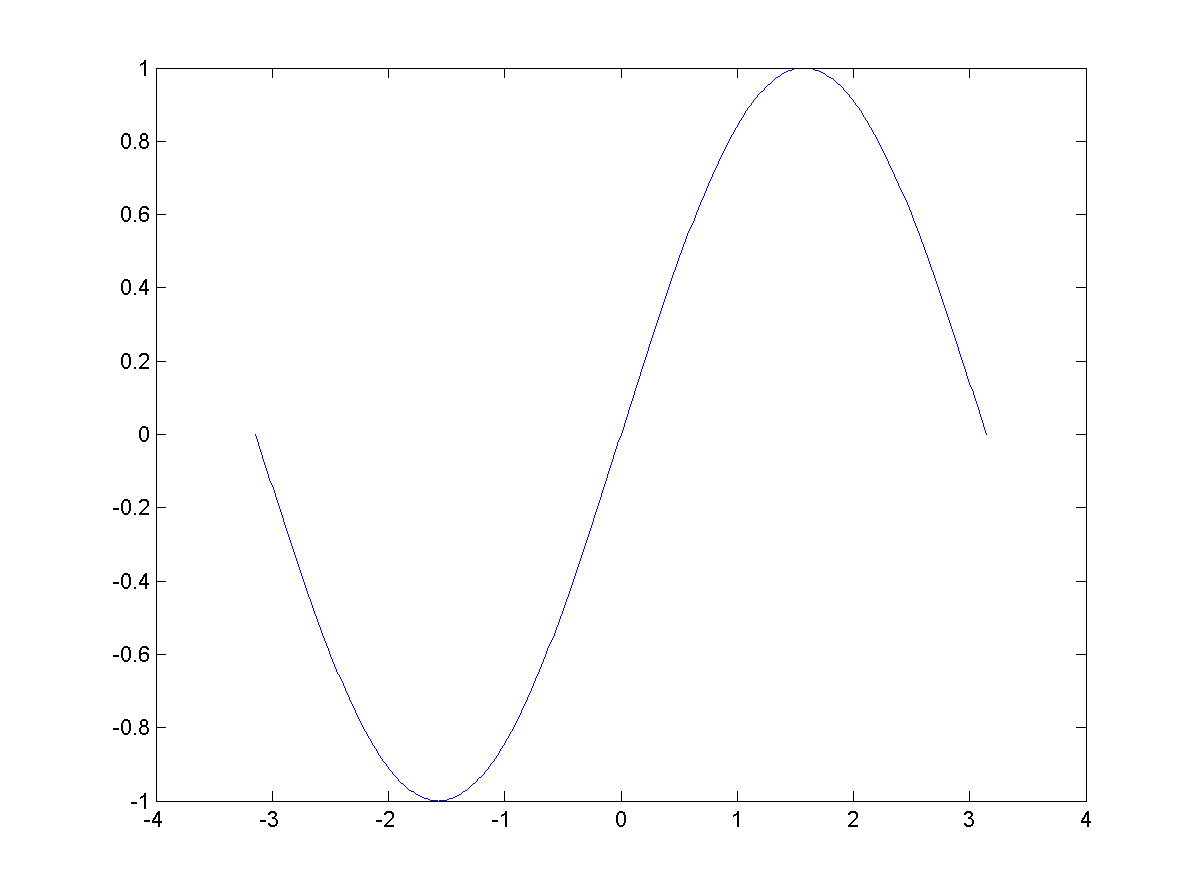
\includegraphics[width=0.65\textwidth]{images/ch4/img_4_1.png}
    \caption{Graficando una función}
    \label{fig:img_4_1}
\end{figure}


\subsection{Graficar más de una función}

Si necesita incluir dos o más gráficas en una misma ventana puede
utilizar el comando \texttt{hold\ on} para permitir que MATLAB
simplemente agregue las gráficas sin borrar las ya existentes, por
ejemplo:

\begin{matlab}
x=-pi:pi/180:pi;
y1=sin(x);
y2=cos(x);
y3=cos(x+pi/3);
hold on
plot(x,y1);
plot(x,y2);
plot(x,y3);
\end{matlab}

\begin{figure}[htbp]
    \centering
    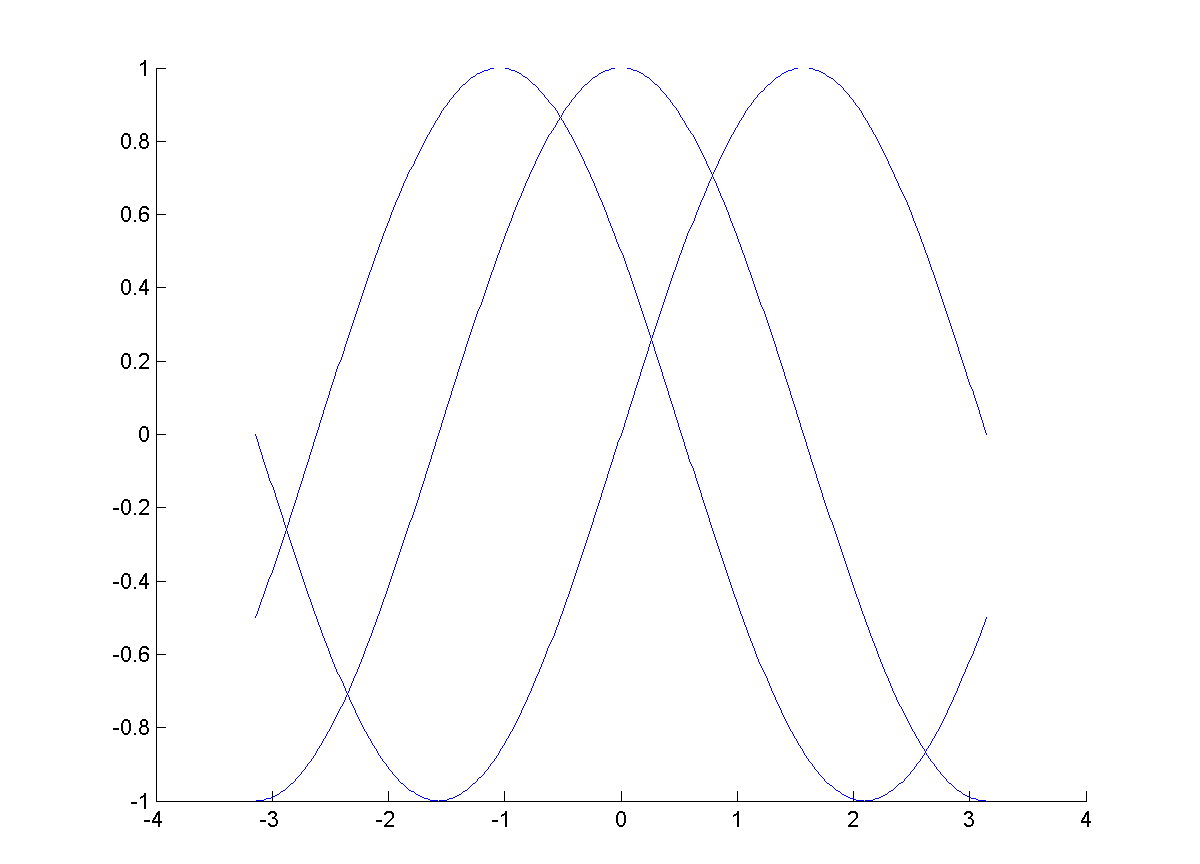
\includegraphics[width=0.65\textwidth]{images/ch4/img_4_2.png}
    \caption{Varias gráficas utilizando \texttt{hold on}}
    \label{fig:img_4_2}
\end{figure}

Lo anterior funciona incluso para cuando se tienen intervalos
diferentes. Si necesita graficar dos o más funciones en un mismo
intervalo, es decir utilizando el mismo vector como variable
independiente, puede utilizar la siguiente forma más compacta para
agregar más de una función sin recurrir al comando descrito con
anterioridad:

\begin{matlab}
x=-pi:pi/180:pi;
y1=sin(x);
y2=cos(x);
y3=cos(x+pi/3);
plot(x,[y1;y2;y3]);
\end{matlab}

\begin{figure}[htbp]
    \centering
    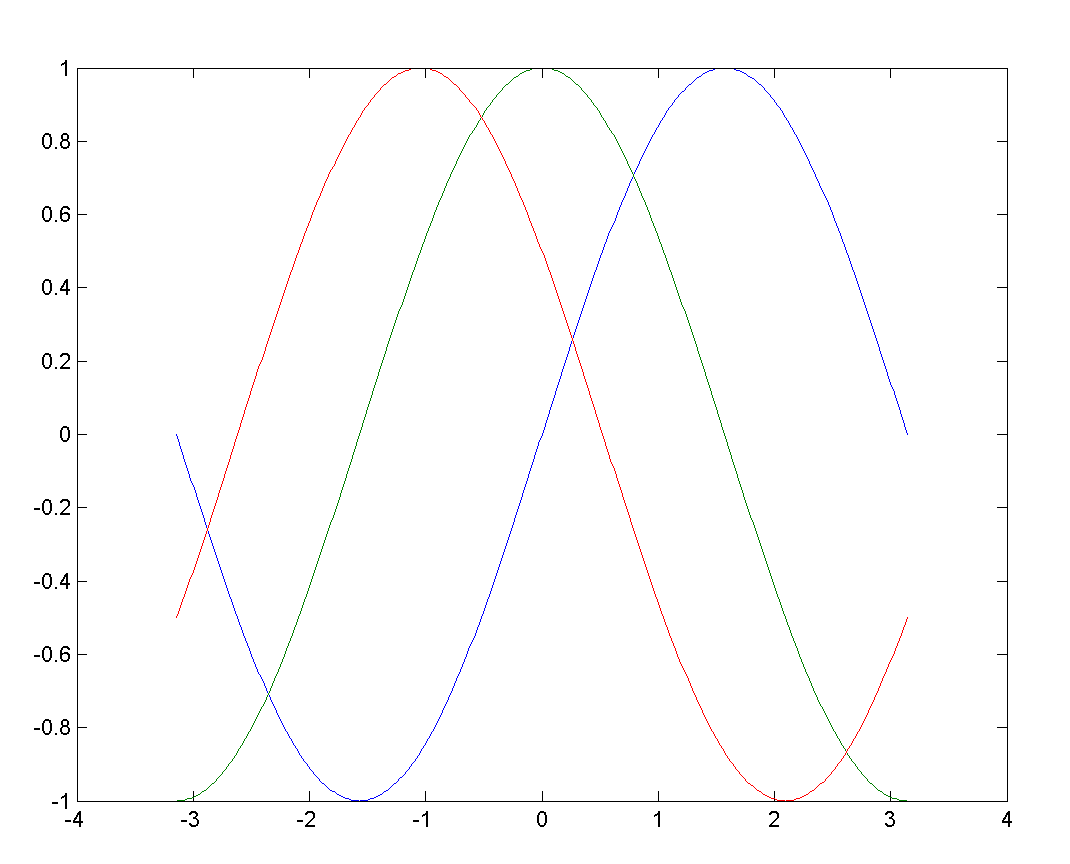
\includegraphics[width=0.65\textwidth]{images/ch4/img_4_3.png}
    \caption{Varias gráficas usando concatenación vectorial}
    \label{fig:img_4_3}
\end{figure}

En lugar de utilizar \texttt{hold on} puede configurar la propiedad
\texttt{NextPlot} del axes de tal manera que las gráficas sean agregadas
sin borrar los objetos que pertenecen al axes. Lo anterior se logra con
la siguiente línea de código:

\begin{matlab}
set(gca, 'NextPlot', 'add');
\end{matlab}

Quizá lo anterior resulte un poco avanzado para comenzar, pero puede
tomarse simplemente como una observación muy útil de que en MATLAB
pueden implementarse diversas soluciones a un mismo problema o
requerimiento.

\section{Configurar propiedades de las gráficas}

\subsection{Añadir etiquetas, leyendas y títulos}

En la sección anterior se han visto los pasos para mínimos para trazar
una gráfica, pero ésta todavía puede resultar poco útil dado que no
contiene información de ningún tipo acerca de los datos graficados. Es
posible añadir etiquetas a los ejes con las funciones xlabel, ylabel y
zlabel, además de poder añadir una identificación de una determinada
curva mediante la función \texttt{legend} e incluso colocar un título en
la parte superior con la función \texttt{title}:

\begin{matlab}
x=-pi:pi/180:pi;
y=sin(x);
plot(x,y);
xlabel('Eje X');
ylabel('Eje Y');
title('Gráfica función seno');
legend('f(x)=sin(x)');
\end{matlab}

\begin{figure}[htbp]
    \centering
    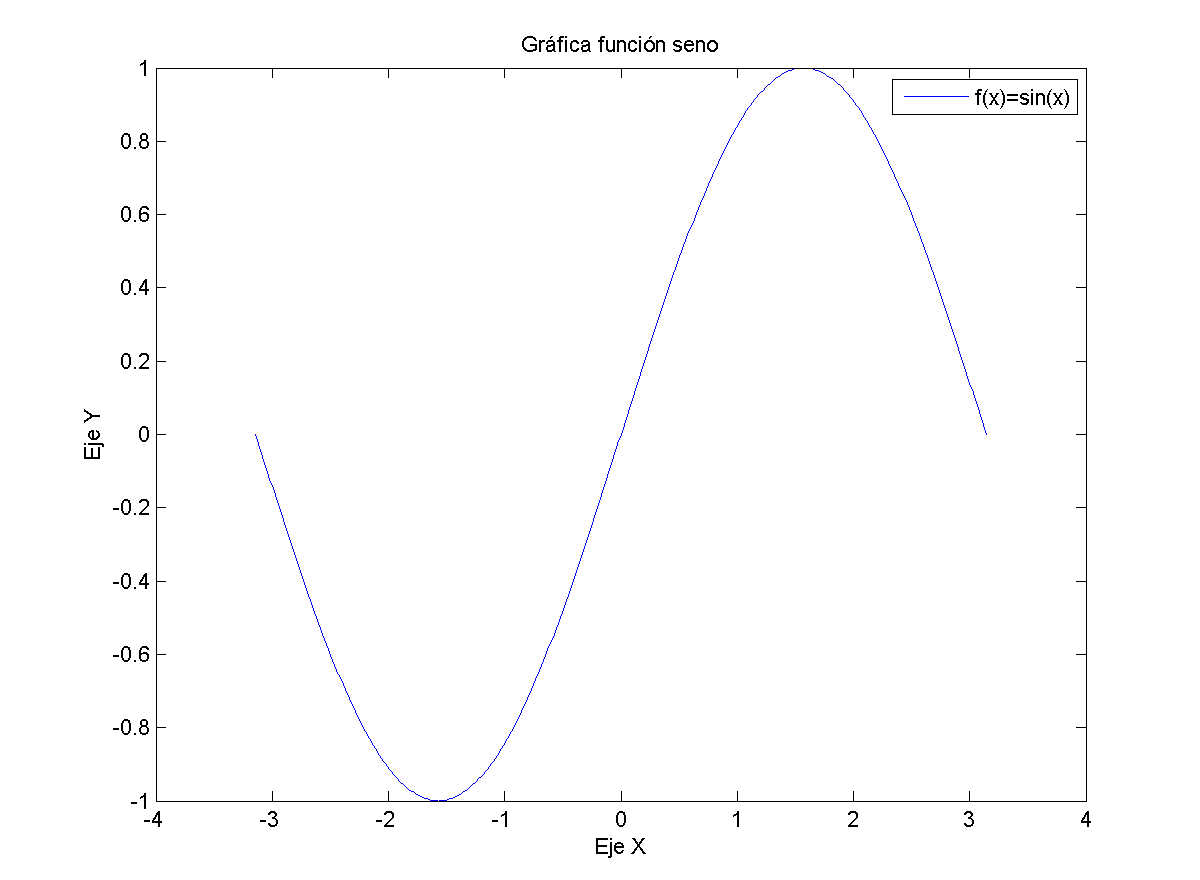
\includegraphics[width=0.65\textwidth]{images/ch4/img_4_4.png}
    \caption{Gráfica con etiquetas y leyenda}
    \label{fig:img_4_4}
\end{figure}

Las gráficas anteriores se han trazado utilizando el estilo por defecto
que emplea MATLAB, es decir, una línea continua en color azul, pero es
posible modificar el color, grosor y el estilo de línea de las gráficas
de modo que se ajuste a los requerimientos o a las exigencias visuales
de cada individuo.

\subsection{Modificando el color de línea}

Para modificar el color de una gráfica basta con añadir como tercer
argumento de la función plot uno de los modificadores de color que se
indican en la siguiente tabla:


\begin{table}[h!]
\centering
% \rowcolors{1}{}{gray!20}
\begin{tabular}{p{3cm} >{\tt}P{3cm}}
\hline
\Centering\bfseries Color  & \normalfont\bfseries Modificador \\
\hline 
Rojo  &  r \\
verde &  g \\
Azul  &  b \\
Cyan  &  c \\
Magenta &  m \\
Amarillo & y \\
Negro  & k \\
Blanco & w \\
\hline
\end{tabular}
\caption{Conversiones entre tipos numéricos}
\end{table}



La sintaxis de la función plot para una línea color verde sería:

\begin{matlab}
plot(x,y,'g');
\end{matlab}

Además de los modificadores anteriores puede utilizarse un vector de
tres elementos RGB para especificar el color, pero en este caso tiene
que especificarse como argumento la propiedad que se modifica, es decir
color, con lo cual la sintaxis bajo este método para trazar una línea
color verde sería como sigue:

\begin{matlab}
plot(x,y,'color',[0 1 0]);
\end{matlab}

\subsection{Configurar ejes (función axis)}

El comando / función axis permite hacer modificaciones a la apariencia y
escala de los ejes en los cuales se trazan las gráficas. La sintaxis
varía dependiendo de la característica a modificar.

\subsubsection{Estableciendo los límites de una gráfica}

Para establecer los límites en los cuales se mostrará una gráfica puede
introducir como argumento de la función axis un vector de 4 (gráficas en
2D) o 6 elementos (gráficas en 3D) con la sintaxis:

\begin{matlab}
axis([xmin xmax ymin ymax]); % Dos dimensiones
axis([xmin xmax ymin ymax zmin zmax]); % Tres dimensiones
\end{matlab}

Los elementos del vector deben ser de tipo double.

\subsubsection{Ocultar o mostrar etiquetas, marcas, y ejes}

Si requiere ocultar los ejes, etiquetas, leyendas y demás marcas en las
gráficas, de tal manera que sólo sea visible la línea trazada, utilice
la función \texttt{axis} con el argumento \texttt{off}. Las siguientes
líneas de código producen la imagen adjunta:

\begin{matlab}
x=linspace(-2*pi,2*pi,200);
y=x.*cos(x);
plot(x,y);
axis off
\end{matlab}

\begin{figure}[htbp]
    \centering
    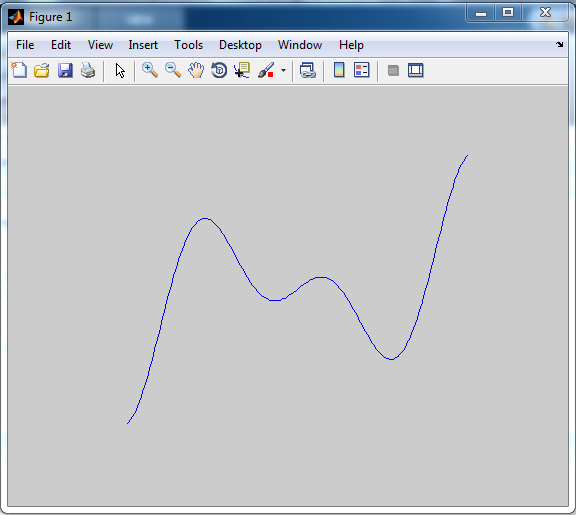
\includegraphics[width=0.5\textwidth]{images/ch4/img_4_5.png}
    \caption{Quitando los axis}
    \label{fig:img_4_5}
\end{figure}

\subsubsection{Escalado de ejes}

Además de permitir una configuración manual de los límites de ejes
mediante la inserción de valores, es posible también establecer límites
mediante modificadores que configuran los ejes y su apariencia de forma
predeterminada. Los más comunes se enlistan y describen en la tabla
siguiente.

\begin{table}[h!]
\centering
\begin{tabular}{ >{\tt}p{3cm} p{5cm} }
\hline
\normalfont\Centering\bfseries Sintaxis  & \Centering\bfseries Descripción \\
\hline 
axis('equal')  & Ajusta el escalado de los ejes de tal modo que sean iguales en cada dirección. \\
axis('square') &  Configura y ajusta la visualización de los ejes a un cuadrado o cubo (3D)  \\
axis('tight') &  Ajusta los ejes al rango de datos disponibles. \\
\hline
\end{tabular}
\caption{Opciones para el escalado de ejes utilizando \texttt{axis}}
\end{table}


\subsection{Añadir texto / anotaciones}

A veces es necesario agregar información extra dentro una gráfica en
forma de texto o anotación. Para ello se puede hacer uso de la función
\texttt{text}, vea el siguiente ejemplo:

\begin{matlab}
t = linspace(0,2*pi);
w = 12;
y = exp(-t).*cos(w*t);
plot(t, y, 'linewidth', 2);
xlabel('Tiempo (s)');
ylabel('Amplitud (mm)');
texto = 'Esto es un texto/anotación';
text(2, 0.5, texto);
\end{matlab}

\begin{figure}[htbp]
    \centering
    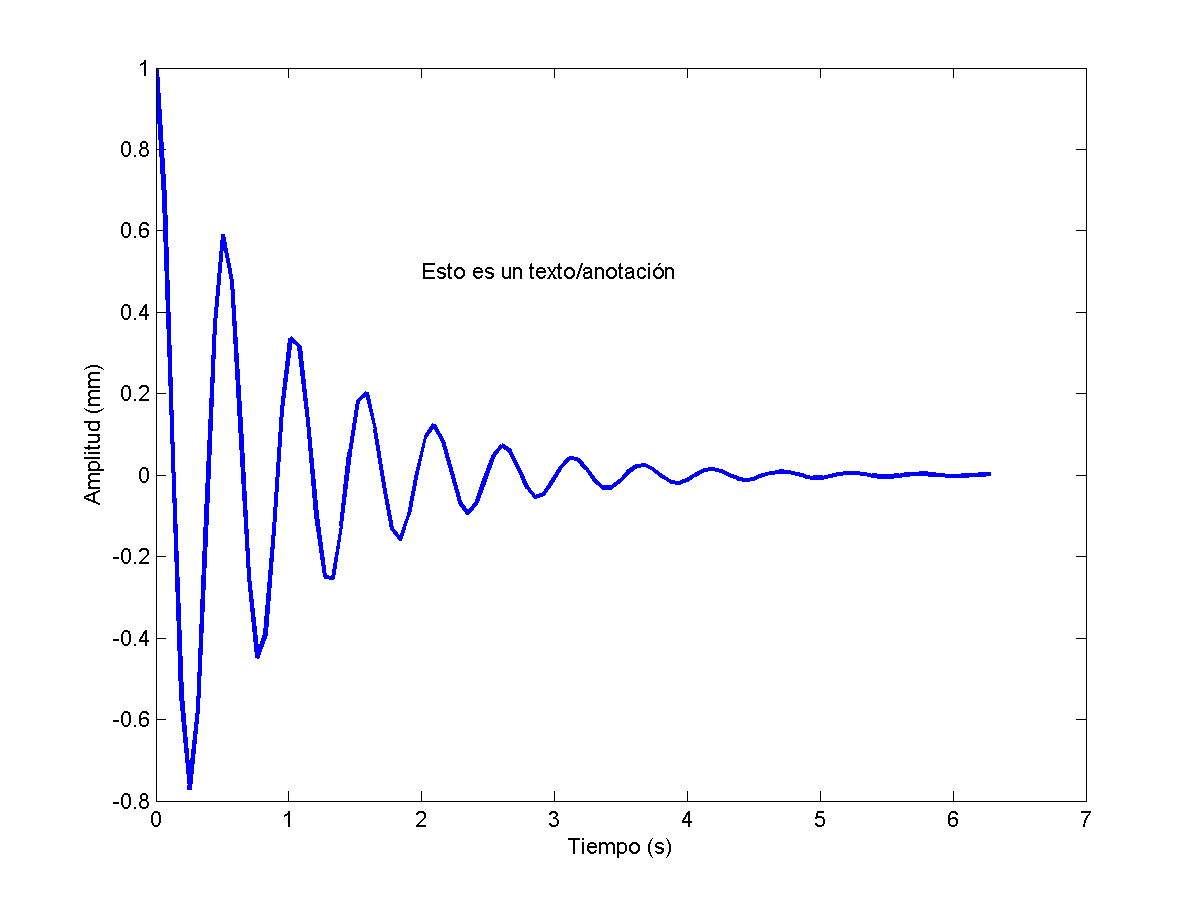
\includegraphics[width=0.75\textwidth]{images/ch4/texto_axes.png}
    \caption{Insertando texto en un axes}
    \label{fig:texto_axes}
\end{figure}

Básicamente la función \texttt{text} necesita tres argumentos de entrada: las 
coordenadas \texttt{x} e \texttt{y} de la posición del texto, y el string 
que contiene el texto que se mostrará en el axes.

\section{Gráficas en coordenadas polares}

En el sistema de coordenadas polares cada punto del plano está definido
por un ángulo y una distancia medidos respecto al eje polar y al polo,
respectivamente. Generalmente para la notación de una ecuación polar se
utilizan la letra griega $\theta$ para el ángulo y una $\rho$ 
para designar la distancia, siendo común la designación $r(\theta)$
para referir a una función en coordenadas polares. \\

Para graficar en coordenadas polares MATLAB dispone de la función polar
cuya sintaxis es:

\begin{matlab}
polar(theta,rho);
\end{matlab}

Ejemplo. Grafique la ecuación $ r(\theta) = \theta $ (espiral).

\begin{matlab}
theta=0:pi/180:6*pi;
r=theta;
polar(theta,r);
\end{matlab}

\begin{figure}[htbp]
    \centering
    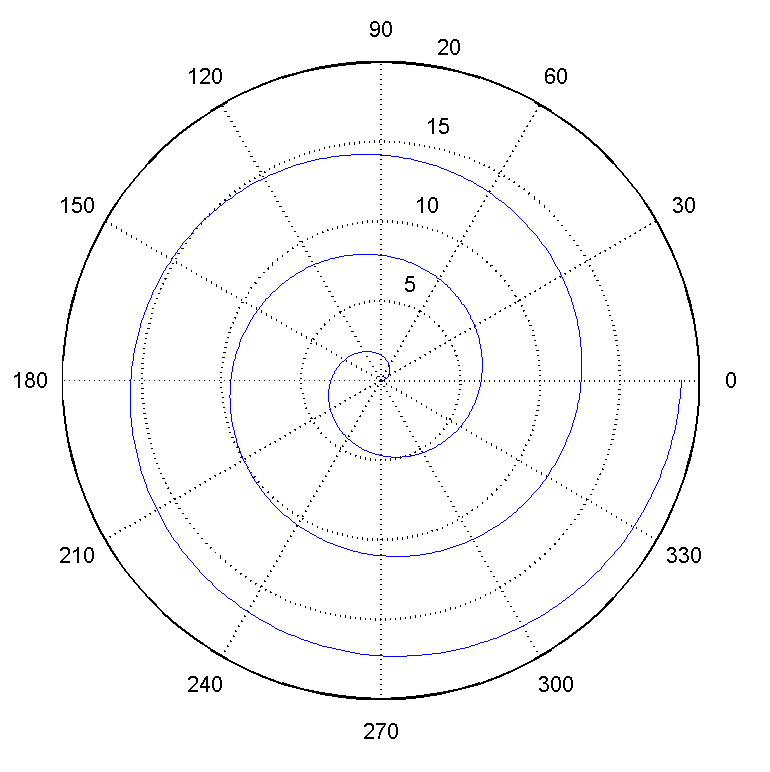
\includegraphics[width=0.6\textwidth]{images/ch4/img_4_6.png}
    \caption{Gráfica de la ecuación $r(\theta) = \theta$}
    \label{fig:img_4_6}
\end{figure}

Pese a que MATLAB cuenta con la función polar para facilitar el trazado
de gráficas en coordenadas polares, es muy sencillo graficar estas
utilizando la función plot con una conversión de coordenadas previa, por
ejemplo, para la misma función anterior:

\begin{matlab}
theta=0:pi/180:6*pi;
r=theta;
x=r.*cos(theta); % Conversión de coordenadas 
y=r.*sin(theta);
plot(x,y);
\end{matlab}

Aunque claro, siempre será mejor utilizar \texttt{polar} dado que esta
automáticamente utiliza los \texttt{axes} de coordenadas polares para
una mejor visualización.


\section{Gráficas de barras}

Las gráficas de barras son una forma de representar gráficamente un conjunto de datos o 
valores y está conformado por barras rectangulares de longitudes proporcionales a los 
valores representados. \\

Para nuestro ejemplo utilizaremos la información proporcionada por la siguiente tabla:

\begin{table}[h!]
\centering
% \rowcolors{1}{}{gray!20}
\begin{tabular}{p{3cm} p{3cm}}
\hline
\Centering\bfseries Asignatura  & \normalfont\bfseries Calificación \\
\hline 
Álgebra & 9 \\
Geometría & 9.5 \\
Cálculo & 10 \\
Estática & 8.5 \\
Química & 8 \\
\hline
\end{tabular}
\caption{Datos para gráfica de barra simple}
\end{table}

MATLAB proporciona la función bar para trazar gráficas de barras, que en su sintaxis más 
simple sólo necesita como argumento un vector con los datos a graficar, véase el ejemplo 
a continuación:

\begin{matlab}
calificaciones=[9,9.5,10,8.5,8];
bar(calificaciones);
\end{matlab}

\begin{figure}[!h]
\centering
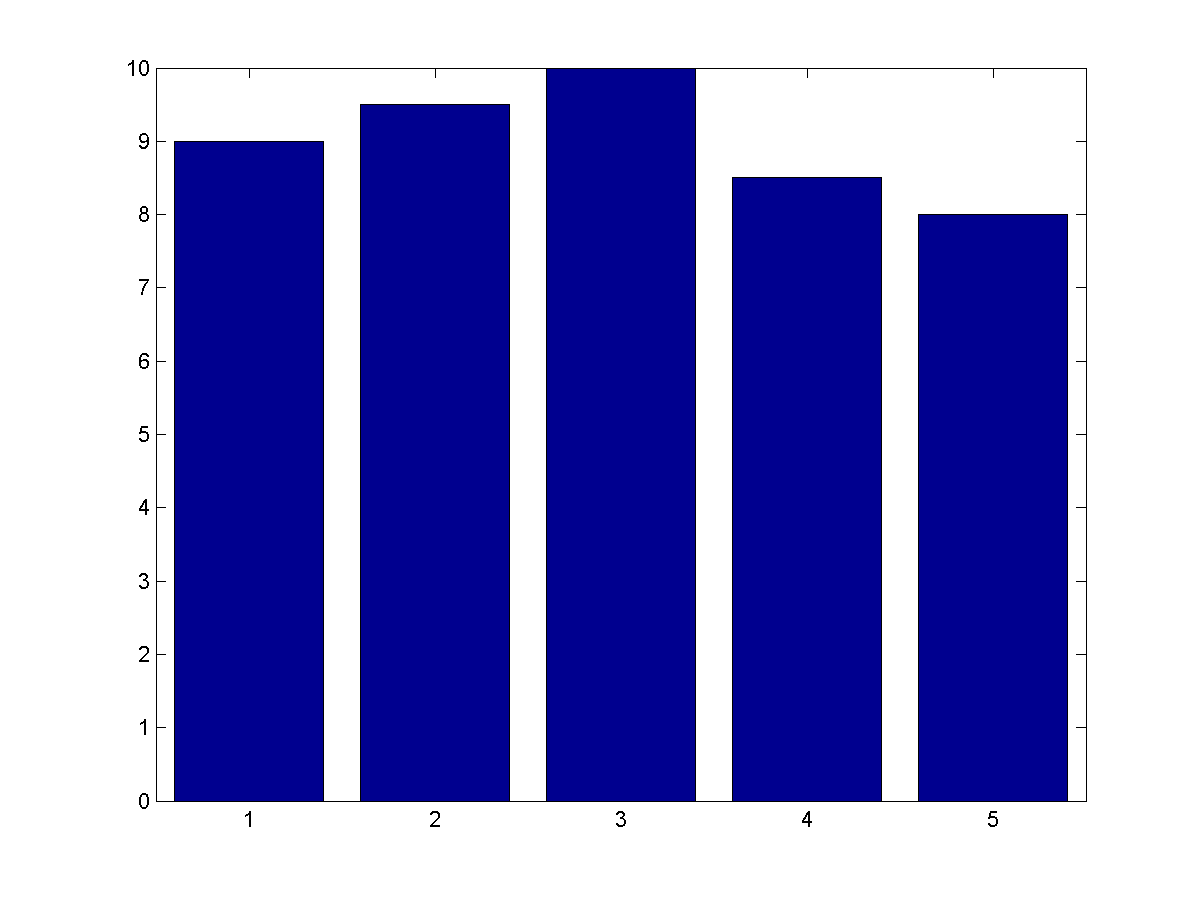
\includegraphics[width=0.6\textwidth]{images/ch4/barra_simple.png}
\caption{Gráficas de barra simple}
\label{fig:barra_simple}
\end{figure}

Lo anterior resulta muy sencillo, pero aún carece de información acerca de los datos que 
se están mostrando. Para añadir una etiqueta a cada dato o barra que se grafica modificaremos 
la propiedad XTickLabel del axes al cuál pertenece el diagrama de barras, en nuestro ejemplo 
esas etiquetas serían el nombre de cada asignatura. Definimos las etiquetas utilizando un 
cell array, veáse el ejemplo:

\begin{matlab}
asignaturas={'Álgebra','Geometría','Cálculo','Estática','Química'};
calificaciones=[9,9.5,10,8.5,8];
h=bar(calificaciones);
set(gca,'XTickLabel',asignaturas);
\end{matlab}

\begin{figure}[!h]
\centering
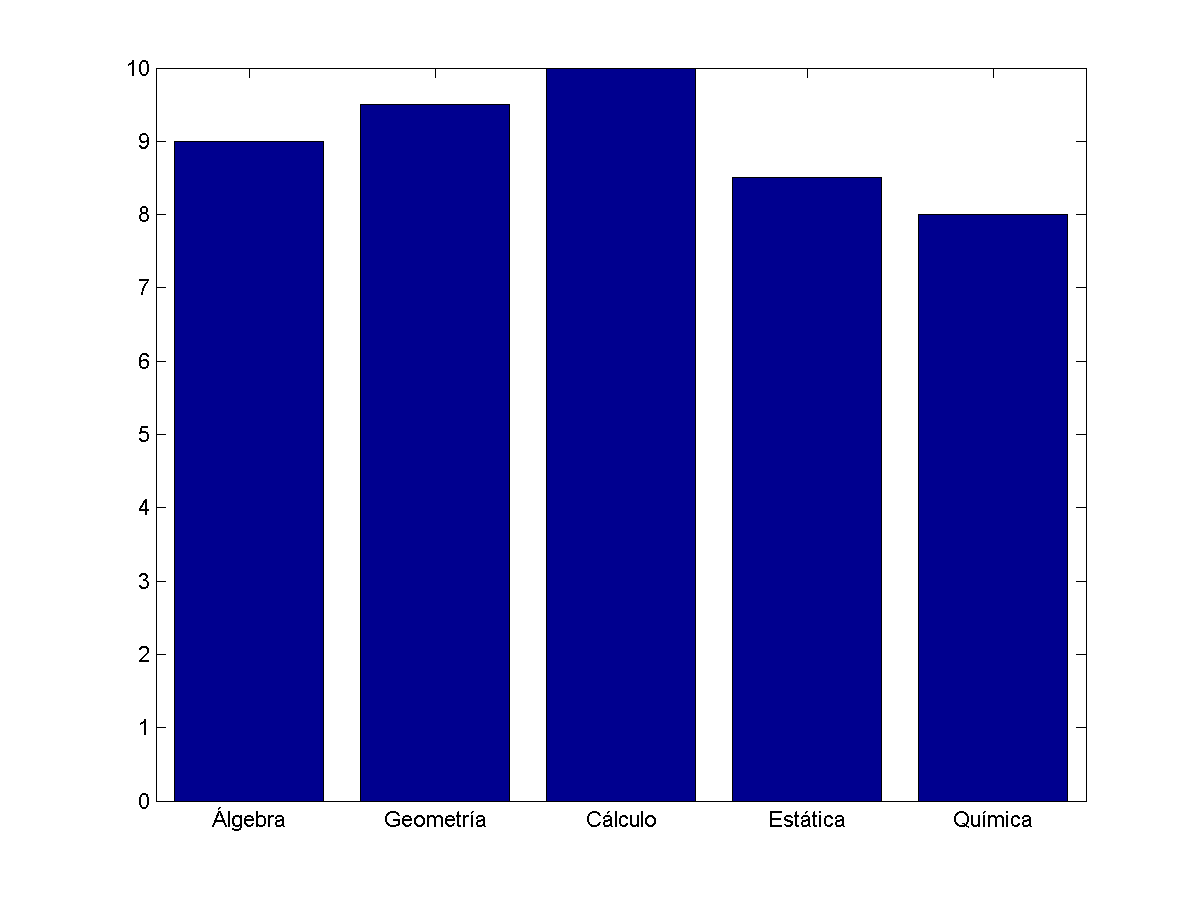
\includegraphics[width=0.6\textwidth]{images/ch4/barra_simple_02.png}
\caption{Gráfica de barra simple, con etiquetas}
\label{fig:barra_simple_02}
\end{figure}

\subsection{Modificar el ancho y color de las barras}

Para modificar el ancho de las barras basta con pasar como segundo argumento de la función bar un 
valor escalar entre 0 y 1, la sintaxis sería:

\begin{verbatim}
bar(X,k);
\end{verbatim}

Donde X es el vector que contiene los valores y k un escalar en el intervalo 0 a 1. \\

Por defecto MATLAB utiliza el color azul para las gráficas de barras, pero existe la posibilidad 
de cambiar el color a conveniencia del usuario. Para ello puede especificarse el color como un 
segundo argumento de la función bar, mediante un especificador de color ('r','g','b','k',...), 
con la sintaxis:

\begin{verbatim}
bar(X,'color');
\end{verbatim}

Donde X es el vector de valor y 'color' el especificador de color mediante caracteres.\\

Si requiere modificar el grosor y color a la vez, puede usar la siguiente sintaxis:

\begin{verbatim}
bar(X,k,'color');
\end{verbatim}

El siguiente ejemplo muestra una gráfica de barras con el ancho y color modificados:

\begin{matlab}
asignaturas={'Álgebra','Geometría','Cálculo','Estática','Química'};
calificaciones=[9,9.5,10,8.5,8];
bar(calificaciones,0.4,'r');
set(gca,'XTickLabel',asignaturas);
title('Calificaciones');
\end{matlab}

\begin{figure}[!h]
\centering
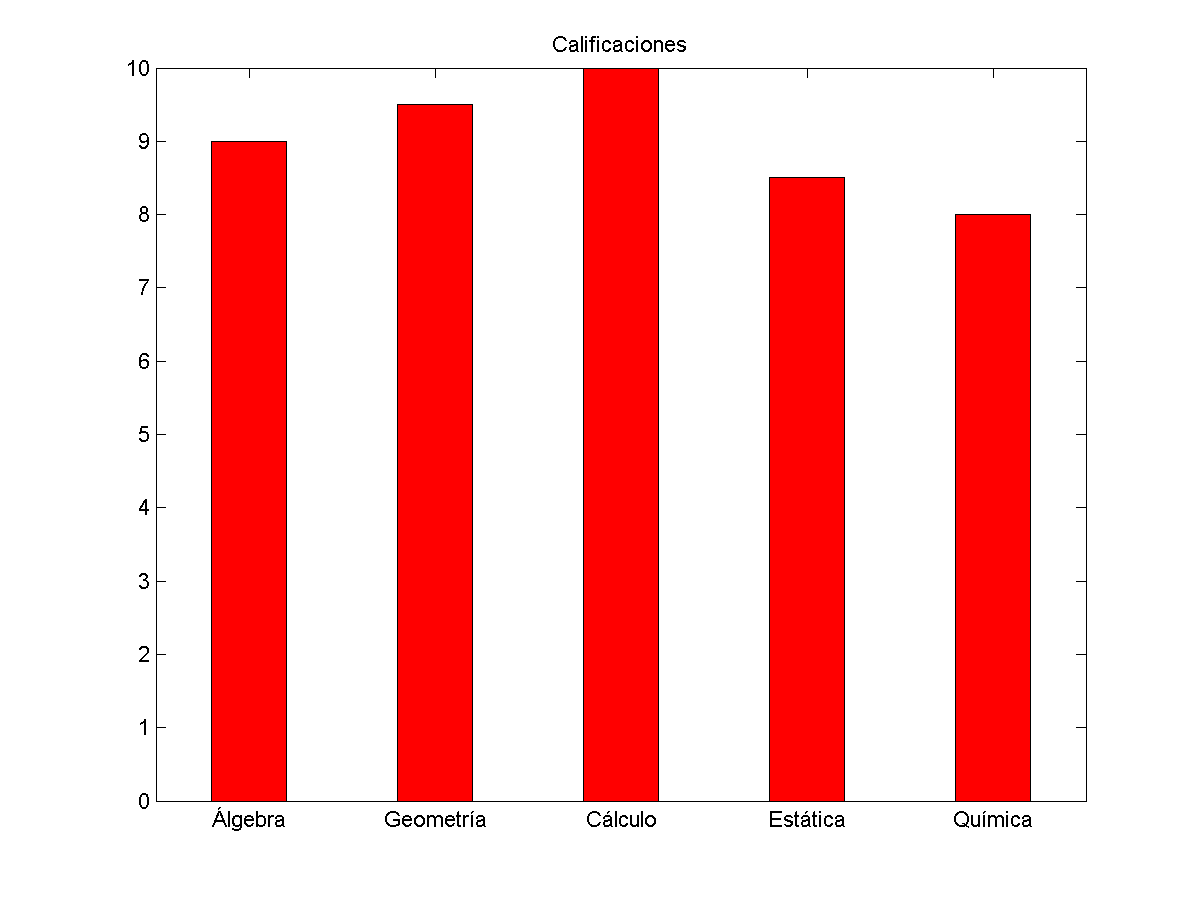
\includegraphics[width=0.6\textwidth]{images/ch4/barra_simple_color.png}
\caption{Gráfica de barra simple, con color y ancho modificado}
\label{fig:barra_simple_color}
\end{figure}

\subsection{Gráficas de barras múltiples}

En ocasiones se necesita representar más de un valor asociado a una misma característica, 
para ello es posible graficar diagramas de barras utilizando matrices en lugar de un vector, 
en donde cada fila proporciona los valores de una misma característica y cada columna pertenece 
a una categoría distinta entre los valores. Para nuestro ejemplo utilizaremos la tabla 
mostrada enseguida.

\begin{table}[h!]
\centering
% \rowcolors{1}{}{gray!20}
\begin{tabular}{p{3cm} P{3cm} P{3cm} P{3cm}}
\hline
\Centering\bfseries \multirow{2}{*}{Alumno} & \normalfont\bfseries \multicolumn{2}{c}{Calificaciones} \\
\cline{2-4}
 & Matemáticas & Física & Química \\
\hline
Ana & 10 & 7 & 9 \\
Jorge & 8 & 8 & 10 \\
Javier & 9 & 9 & 8 \\
\hline
\end{tabular}
\caption{Datos para gráfica de barra simple}
\end{table}

En la tabla anterior cada alumno tiene tres calificaciones asociadas en diferentes asignaturas. 
El siguiente ejemplo muestra cómo trazar la gráfica de barras correspondiente:

\begin{matlab}
nombres={'Ana','Jorge','Javier'};
Ana=[10,7,9];
Jorge=[8,8,10];
Javier=[9,9,8];
bar([Ana;Jorge;Javier]);
set(gca,'XtickLabel',nombres);
\end{matlab}

\begin{figure}[!h]
\centering
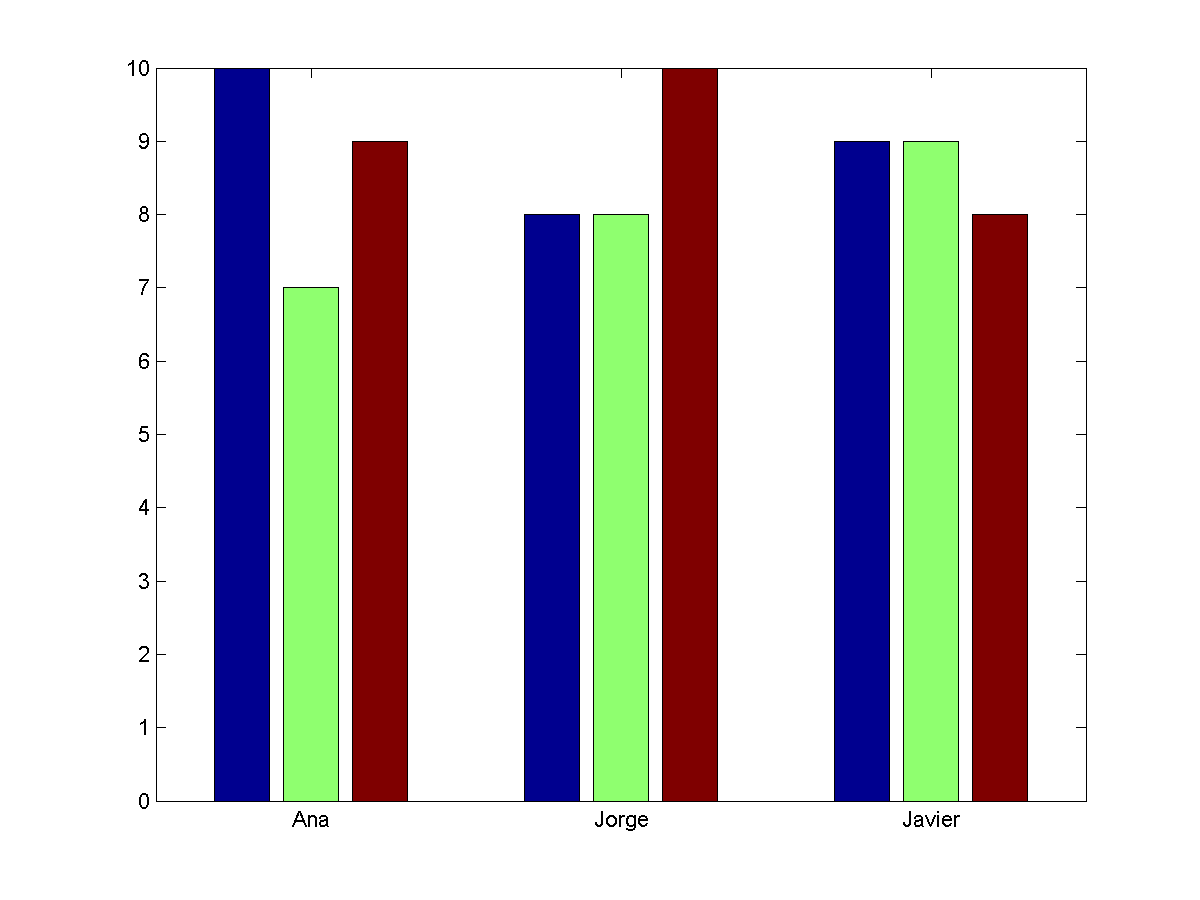
\includegraphics[width=0.6\textwidth]{images/ch4/barra_multiple.png}
\caption{Gráfica de barras múltiples}
\label{fig:barra_multiple}
\end{figure}

\section{Gráficas de pastel/tarta}


\section{Polígonos}



\section{Gráficas de superficies: una primera aproximación}

La representación gráfica de una función de dos variables 
$f(x,y)$ es una superficie trazada en un espacio
tridimensional, resultante de la evaluación de la función en intervalos
determinados para cada variable independiente. \\

A manera de ejemplo crearemos una matriz con los valores resultantes de
la evaluación de la función en un punto específico; comenzaremos
definiendo una función anónima de dos variables y enseguida utilizar
ciclos for anidados para evaluar la función en cada punto. Véase el
ejemplo mostrado a continuación:

\begin{matlab}
f=@(x,y) x.^2+y.^2;
X=-5:0.2:5;
Y=-5:0.2:5;
for i=1:length(X)
    for j=1:length(Y)
        Z(i,j)=f(X(i),Y(j));
    end
end
surf(Z);
\end{matlab}

\begin{figure}[htbp]
    \centering
    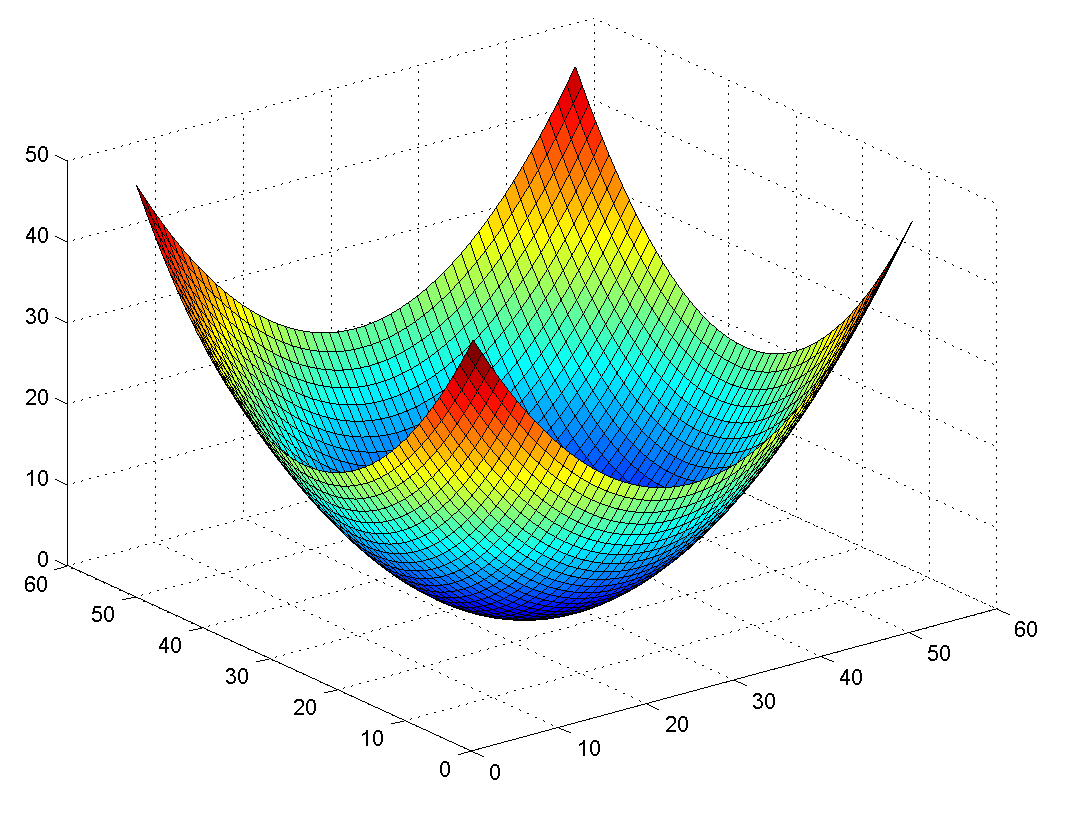
\includegraphics[width=0.6\textwidth]{images/ch4/img_4_7.png}
    \caption{Gráfica de una superficie}
    \label{fig:img_4_7}
\end{figure}

La función \texttt{surf} en el ejemplo anterior recibe como argumento de
entrada una matriz bidimensional cuyos valores corresponden a cada punto
evaluado. El código mostrado es funcional y muy entendible para un
usuario que comienza en el mundo MATLAB, e incluso podría hacerse más
``portable'' o ``reutilizable'' si se definiese como una función, pero
presenta ciertos inconvenientes: los ciclos \texttt{for} en MATLAB son
generalmente conocidos por su lentitud, y más aún, en este caso se
tienen dos ciclos for anidados. Debido a ello, MATLAB proporciona
funciones que realizan la ``tarea'' de evaluar una función de dos
variables en un rango definido mediante la implementación de rejillas
bidimensionales (\texttt{meshgrid}), estas funciones se encuentran
optimizadas mediante la técnica de vectorización y permiten una
ejecución notablemente más veloz.

\section{Gráficas de superficies, utilizando \texttt{meshgrid}}

En el apartado anterior se ha visto como trazar superficies utilizando
ciclos for anidados para crear la matriz que define los valores de la
función de dos variables, pero ahora vamos a optimizar nuestro código
utilizando la función \texttt{meshgrid} para definir el rango de valores
a evaluar, la sintaxis de \texttt{meshgrid} es:

\begin{matlab}
>> [X,Y]=meshgrid(ix,iy);
\end{matlab}

Donde X e Y son las matrices que definen el rango para las variables
independiente y que se utilizarán para evaluar en una determinada
función, ix e iy son vectores que definen el intervalo a evaluar de cada
variable independiente. A continuación se muestra un ejemplo completo de
cómo utilizar meshgrid en conjunto con surf para crear una gráfica de la
función  $f(x,y)=cos(x) sin(y)$:

\begin{matlab}
ix=0:0.2:10;
iy=-5:0.2:5;
[X,Y]=meshgrid(ix,iy);
Z=cos(X).*sin(Y);
surf(X,Y,Z);
\end{matlab}

\begin{figure}[htbp]
    \centering
    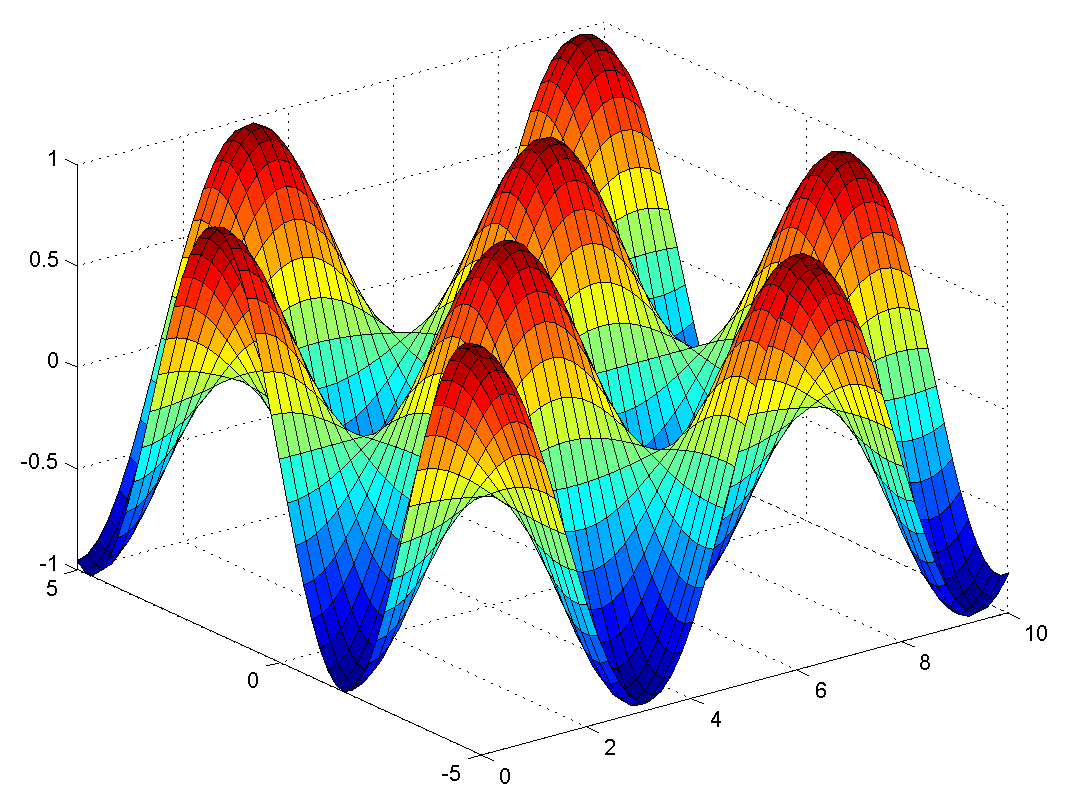
\includegraphics[width=0.6\textwidth]{images/ch4/img_4_8.png}
    \caption{Gráfica de la superficie $f(x)=cos(x) sin(y)$}
    \label{fig:img_4_8}
\end{figure}

Note que las operaciones de multiplicación o división deben estar
vectorizadas, es decir, colocar un punto antes de cada operador
correspondiente para indicar que se debe operar elemento a elemento. De
lo contrario MATLAB devolverá un error o más grave aún: un resultado
incorrecto. \\

Si ambos intervalos X e Y son iguales, puede proporcionar solo un
argumento a la función meshgrid, es decir, es lo mismo tener esto:

\begin{matlab}
[X,Y]=meshgrid(1:10,1:10);
\end{matlab}

que lo siguiente:

\begin{matlab}
[X,Y]=meshgrid(1:10);
\end{matlab}

Claro que por cuestiones de comodidad sería preferible esta última,
aunque quizá afecte un poco la legibilidad de un programa de mayores
dimensiones, pero vamos, nada ``catastrófico''.

\section{Mapas de colores y sombreado}

\subsection{Mapas de colores}

Un mapa de color es, en su definición más simplista, una matriz de m x 3
elementos cuyos valores se encuentran en el intervalo de 0 a 1, y donde
cada fila representa un vector que especifica un color en el formato o
modelo de color RGB. Pero, aquí la cuestión interesante es ¿para qué
sirve un mapa de color?; así pues, un mapa de color no es más que un
conjunto de colores que habrán de utilizarse para ``pintar'' una
superficie de acuerdo a sus valores, pudo notar que en las superficies
trazadas en los apartados anteriores se utiliza un color rojo para los
valores más grandes y un color azul para los más pequeños, pasando por
otras tonalidades para valores intermedios. Debe saber que esa ``forma
de colorear'' la superficie está definida mediante un mapa de color por
defecto, generalmente jet. Aparte de jet MATLAB cuenta con otros mapas
de colores predefinidos que se muestran a continuación:

\begin{figure}[htbp]
\centering
\includegraphics[width=0.25\textwidth]{images/ch4/img_4_9.png}
\caption{}
\end{figure}

Si teclea en MATLAB el nombre de cualquiera de los mapas de colores
mostrados se devuelve una matriz de 64x3 elementos de tipo double, por
ejemplo:

\begin{matlab}
>> map_color=hsv;
>> whos map_color
  Name            Size            Bytes  Class     Attributes

  map_color      64x3              1536  double          
\end{matlab}

Pero todo esto no tiene efecto sobre alguna superficie dibujada, para
cambiar o configurar el mapa de color actual puede utilizar la función
\texttt{colormap}, pasando un mapa de color como argumento, por ejemplo:

\begin{matlab}
[X,Y]=meshgrid(0:0.2:3*pi);
Z=cos(X).*sin(Y);
surf(X,Y,Z);
colormap(hot);
\end{matlab}

\begin{figure}[htbp]
    \centering
    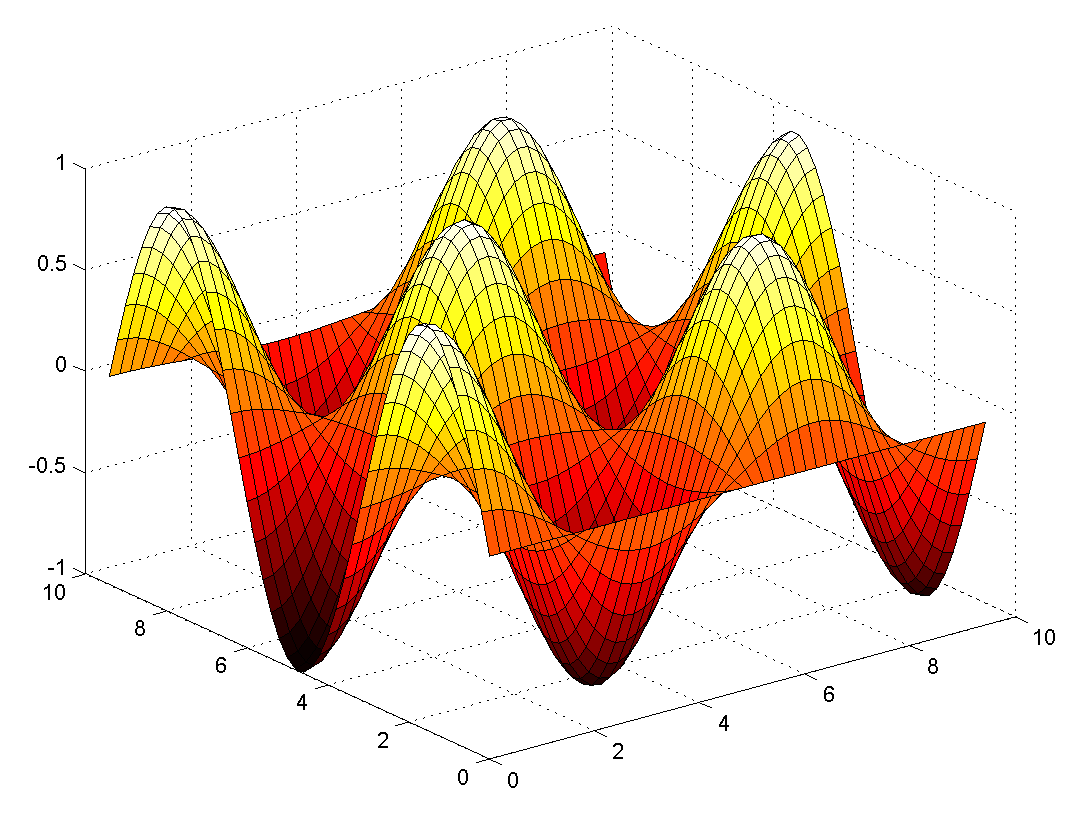
\includegraphics[width=0.6\textwidth]{images/ch4/img_4_10.png}
    \caption{Utilizando el mapa de color \texttt{hot}}
    \label{fig:label}
\end{figure}

Interesante, sobre todo para quienes deseen darle a sus gráficos una
mayor calidad estética o acorde a los datos que esté representando. \\

Si por alguna razón ninguno de los mapas de colores predefinidos le
``convence'', puede definir su propio mapa de color sin muchas
complicaciones, para ello debe crear una matriz de m x 3 elementos donde
cada fila contenga información acerca de un color en formato RGB,
tomando en cuenta que el color ubicado en la primera fila será asignado
al valor más pequeño y la última fila al mayor. Revise el siguiente
ejemplo en el cual se define un mapa de color mediante cierta secuencia:

\begin{matlab}
Z=membrane;
surf(Z);
v=(1:10)'/10;
cmap=[v flipud(v) flipud(v)];
colormap(cmap);
\end{matlab}

\begin{figure}[htbp]
    \centering
    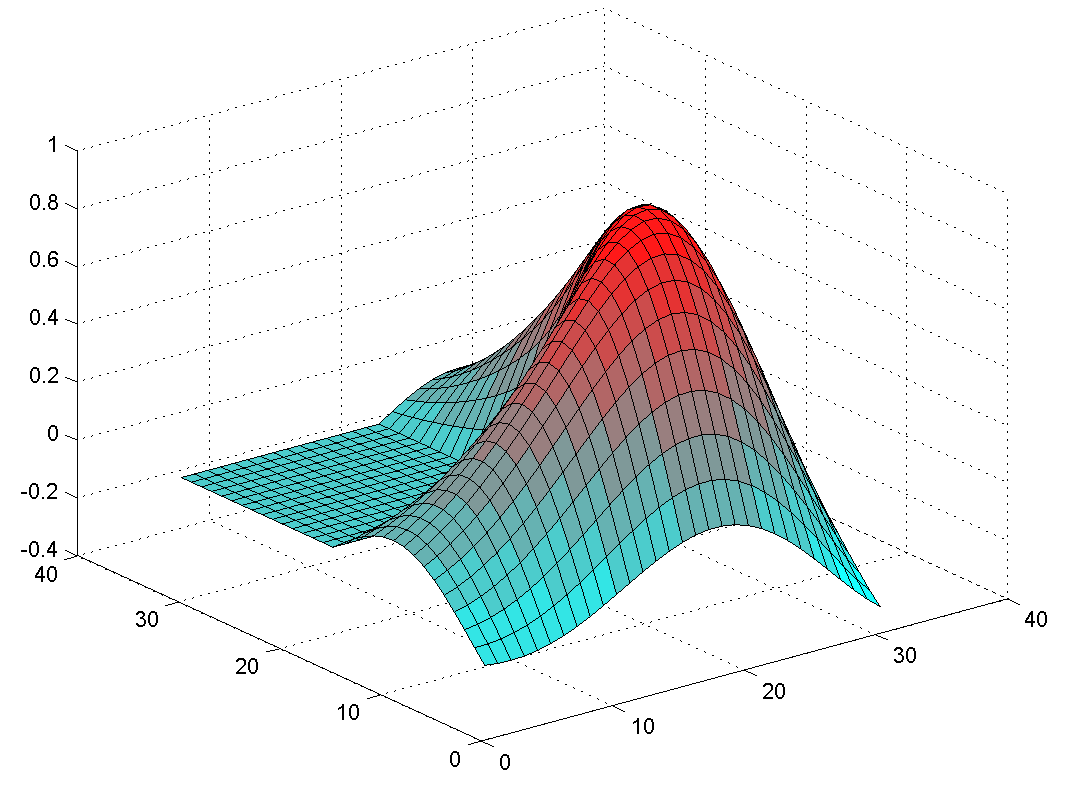
\includegraphics[width=0.75\textwidth]{images/ch4/img_4_11.png}
    \caption{Utilizando un mapa de color personalizado}
    \label{fig:img_4_11}
\end{figure}

El resultado es una interesante variación de tonalidades ¿azul? a rojo.
Por supuesto que usted tiene todas las libertades para experimentar con
diversas secuencias de colores y ``adoptar'' la que mejor le resulte.

\subsection{Sombreado}

Para efectos de esta sección, con sombreado se refiere a la forma en que
MATLAB \emph{pinta} o \emph{rellena} los diversos componentes o parches
(patch) que conforman una superficie. \\

En MATLAB existen tres tipos de sombreado que pueden controlarse
mediante la función \texttt{shading}, los cuales son:

\begin{itemize}
\tightlist
\item
  faceted
\item
  flat
\item
  interp
\end{itemize}

El tipo \texttt{faceted} es el sombreado por defecto, y se caracteriza
por pintar cada parche de la superficie utilizando un color sólido de
relleno y un borde en color negro. \\

El tipo \texttt{flat} funciona de manera similar al anterior, con la
diferencia que el borde adquiere el mismo color que el interior del
parche. \\

Y el tipo \texttt{interp} se vale de una interpolación de la matriz que
define el mapa de color actual para pintar de forma cuasi-continua y con
variaciones menos ``bruscas'' a cada parche, de hecho con este tipo de
sombreado es imposible distinguir cada pieza que compone la superficie. \\

La función \texttt{shading} sólo necesita como argumento el tipo de
sombreado, por ejemplo:

\begin{matlab}
>> shading('flat')
\end{matlab}

Incluso acepta la notación de comandos, es decir, la siguiente forma
también es válida:

\begin{matlab}
>> shading flat
\end{matlab}

\section{Planos}

\section{Esferas}

\section{Cilindros}

\section{Curvas de nivel}

\section{Subplots: múltiples axes}

\section{Gráficos interactivos}
% \chapter{Exportar e importar variables y datos}

\section{Guardar y cargar variables del workspace: save y load}

Durante una sesión ordinaria utilizando MATLAB las variables creadas se
almacenan en el workspace y están disponibles para usarse, siempre y
cuando no se haya utilizado algún comando para borrar las variables, sin
embargo cuando se cierra la sesión de MATLAB las variables del workspace
son borradas y no es posible utilizarlas posteriormente. Para poder
``conservar'' una variable creada y utilizarla en cálculos futuros, es
posible guardar estas en archivos MAT nativos del lenguaje MATLAB; lo
anterior se logra utilizando la función save, cuya sintaxis es:

\begin{matlab}
save('nomb_arch.mat','nvar');
\end{matlab}

Siendo \texttt{nomb\_arch} el nombre del archivo en el cual se guardarán
las variables, que incluso puede ser una combinación de una dirección
absoluta o relativa y el nombre del archivo; nvar es el nombre de la
variable o variables a ser guardadas. Si desea guardar todas las
variables actuales puede omitir el resto de argumentos y solo utilizar
el nombre del archivo. Las siguientes líneas ejemplifican cómo hacer uso
de la función save:

\begin{matlab}
>> k=1.37;
>> A=[1 2 -1;0 1 0;-2 0 0];
>> C={'A','B','C'};
>> save('arch1.mat'); % Guarda todas las variables
>> save('arch2.mat','A'); % Guarda sólo la variable A
\end{matlab}

El contenido de los archivos MAT puede cargarse y guardar en el
workspace mediante la función \texttt{load}, con la sintaxis:

\begin{matlab}
load('narch.mat','vars');
\end{matlab}

Donde narch es el nombre del archivo y vars la(s) variable(s) a cargar
en el workspace. Si únicamente se indica como argumento el nombre del
archivo, entonces se cargan todas las variables contenidas en el
archivo. Para ejemplificar el uso de load utilizaremos el archivo
``arch1.mat'' creado anteriormente:

\begin{matlab}
>> load('arch1.mat');
>> whos % Verificamos las variables cargadas en el workspace
  Name      Size            Bytes  Class     Attributes
  A         3x3                72  double              
  C         1x3               342  cell                
  k         1x1                 8  double       
\end{matlab}

Puede asignarse la función load a una variable, con lo cual todo el
contenido del archivo MAT se guardara en una estructura con cada una de
las variables como campos. Para el mismo ejemplo anterior se tiene:

\begin{matlab}
>> S=load('arch1.mat');
>> S
S = 
    k: 1.3700
    A: [3x3 double]
    C: {'A'  'B'  'C'}
>> whos 
  Name      Size            Bytes  Class     Attributes
  S         1x1               950  struct       
\end{matlab}

\section{Carpetas y archivos, operaciones básicas.}

\subsection{Cambiar el directorio o carpeta}

La función \texttt{cd} cambia la carpeta actual (Current Folder),
utilizando como argumento una cadena de caracteres con la dirección
absoluta o relativa del nuevo directorio de trabajo. La sintaxis es:

\begin{matlab}
cd('Nueva Carpeta');
\end{matlab}

Un ejemplo se muestra enseguida:

\begin{matlab}
cd('C:\Users\User\Documents\MATLAB');
\end{matlab}

Si solo se pone la instrucción \texttt{cd} sin argumentos, entonces
MATLAB devuelve un string con la carpeta actual. \\

\begin{informacion}{Direcciones absolutas y relativas}
Una dirección absoluta es aquella representada mediante
toda la ruta  que la describe, incluyendo al directorio
raíz. En Windows las  direcciones absolutas suelen ser de
la forma \texttt{C:/Users/User/\ldots{}}, donde  User es
el nombre del usuario registrado en el equipo. Las direcciones
 relativas se expresan con respecto a una determinada
carpeta, por  ejemplo, si estamos ubicados dentro de una
carpeta Documents cuya  dirección absoluta es
\texttt{C:/Users/User/Documents} y dentro de ella 
tenemos una carpeta llamada MATLAB, la forma relativa de referirnos a
 esta carpeta sería simplemente con la cadena
\texttt{MATLAB}.
\end{informacion}

\subsection{Crear y eliminar carpetas}

A estas alturas, crear y manipular carpetas resulta una tarea trivial
cuando se ejecuta en el ambiente de cualquier sistema operativo que
maneje, incluso en el Current Folder de MATLAB puede crear, modificar y
eliminar carpetas tal como lo hace normalmente. Pese a lo anterior, en
diversas situaciones puede ser necesario crear carpetas mediante la
ejecución de código a través de comandos y/o funciones destinadas para
tal fin. En MATLAB se dispone de la función mkdir que permite crear
carpetas utilizando el nombre de la misma como argumento, por ejemplo:

\begin{matlab}
>> mkdir('Mis Cursos');
\end{matlab}

La instrucción anterior crea una carpeta llamada Mis Cursos en el
directorio actual de trabajo. Es posible también pasar como argumento la
dirección absoluta o relativa de la carpeta a crear:

\begin{matlab}
>> mkdir('Mis Cursos/MATLAB');
\end{matlab}

En la línea anterior se crea dentro de la carpeta Mis Cursos una cuyo
nombre es MATLAB. \\

Habitualmente en la programación se hace necesario considerar la mayoría
de las situaciones posibles para dar una mayor robustez al código, y con
ello hacerlo más autónomo y eficiente. Imagine que necesite crear
carpeta a la cual le asignará un nombre determinado, entonces, hay una
posibilidad, aun siendo mínima, que ya exista una carpeta con ese mismo
nombre. MATLAB no remplazará la carpeta existente por la nueva, pero le
mostrará un mensaje de error o advertencia y posiblemente detenga la
ejecución del código. Para evitar lo anterior puede comprobar antes si
existe un directorio con ese nombre y mediante una sentencia de control
especificar las acciones a ejecutar en cada caso. Véase el ejemplo
siguiente en donde se realiza la comprobación mediante la función isdir:

\begin{matlab}
if ~isdir('Cursos')
    mkdir('Cursos');
else
    mkdir(['Cursos','2']);
end
\end{matlab}

Para eliminar una carpeta MATLAB proporciona la función rmdir cuyo
argumento es la carpeta a eliminar, o bien la dirección absoluta o
relativa de la misma. Por ejemplo, si quiere eliminar una carpeta
llamada Cursos, ubicada en el directorio actual:

\begin{matlab}
>> rmdir('Mis Cursos');
\end{matlab}

Lo anterior funciona para carpetas que no contengan subcarpetas, de lo
contrario MATLAB le devolverá un mensaje de error como el siguiente:

\begin{matlab}
>> rmdir('Mis Cursos')
Error using rmdir
No directories were removed.
\end{matlab}

Para borrar una carpeta que contenga subcarpetas debe incluir un segundo
argumento, siendo este una ``s'' entre comillas simples, como se
muestra:

\begin{matlab}
>> rmdir('Mis Cursos','s');
\end{matlab}

\subsection{Crear y eliminar carpetas}

Conocer los archivos y directorios dentro de una carpeta suele ser una
necesidad básica para cualquier programador, sobre todo para el
almacenamiento y organización de archivos de trabajo. MATLAB cuenta con
funciones que facilitan la tarea de consultar el contenido de una
carpeta, entre las más comunes están \texttt{dir}, \texttt{ls} y
\texttt{what}, a continuación veremos la utilidad de cada una.

\subsubsection{La función dir}

La función dir, sin argumentos de salida pedidos de forma explícita y
sin argumentos de entrada, devuelve en pantalla una lista de archivos y
directorios contenidos en el \textbf{Current Folder}. Véase el ejemplo:

\begin{matlab}
>> dir
.               grlev.png       matricesEx.m    
..              idmat.m         ordseleccion.m  
datos.txt       img.png         unos.m     
\end{matlab}

No obstante, si asignamos la función dir a una variable cualesquiera
entonces se guardará una estructura que contiene información acerca del
nombre, tamaño, fecha de modificación, entre otras características de
los archivos contenidos en el directorio actual.

\begin{matlab}
>> S=dir
S = 
9x1 struct array with fields:
    name
    date
    bytes
    isdir
    datenum
\end{matlab}

Para acceder a la información de cada archivo puede hacerlo mediante el
índice correspondiente, por ejemplo:

\begin{matlab}
>> S(3)
ans = 
       name: 'datos.txt'
       date: '01-oct-2014 15:13:46'
      bytes: 74
      isdir: 0
    datenum: 7.3587e+05
\end{matlab}

Desde luego que esta forma de utilizar la función \texttt{dir} es mucho
más útil que aquella que simplemente muestra en pantalla la información. \\

Es posible además especificar como argumento la dirección de la cual se
requiere información (una distinta al Current Folder) e inclusive
utilizar comodines para visualizar solo archivos con una determinada
extensión, por ejemplo:

\begin{matlab}
>> dir('C:/Users/User/Documents/MATLAB/*.png')
ayuda.png  img.png 
\end{matlab}

La instrucción anterior busca en la carpeta MATLAB todos los archivos
con extensión PNG (imágenes), sin importar el nombre de estos, e ignora
cualquier otro tipo de archivo o directorio ubicado en esta misma
carpeta. Ahora, revise el siguiente ejemplo:

\begin{matlab}
>> dir('C:/Users/User/Documents/MATLAB/m*')
MATLAB TYP           Mecanismos           My File Exchange     
MATLAB_Function.m    Mis Apuntes          matrizBinaria.m      
Matemáticas Básicas  Moler Books          miHist.m       
\end{matlab}

Como puede observar, MATLAB devuelve todos aquellos archivos y carpetas
cuya primera letra sea \textbf{m}, sin importar ninguna otra
característica.

\subsection{Mover, copiar y eliminar
archivos}\label{mover-copiar-y-eliminar-archivos}

Mover, copiar y eliminar archivos son tareas muy comunes para cualquier
usuario de un ordenador y que pueden ejecutarse con mucha facilidad de
forma manual. No obstante, utilizar la programación para estas tareas
puede resultar de mucha ayuda, sobre todo cuando se necesita trabajar
con grandes volúmenes de datos y/o archivos, ya que permite automatizar
los procedimientos y ejecutarlos en un tiempo impensable para un
individuo. Claro que se podría justificar que existen formas para
seleccionar todos los archivos de un directorio y colocarlos en otro de
forma muy sencilla aun cuando fuesen millares de archivos, pero ¿qué
pasa si solo necesitamos trabajar con archivos cuyo nombre cumpla una
determinada característica o patrón? ¿O con archivos de un tamaño
específico? ¿O con una fecha de modificación reciente?, incluso con
combinaciones de las anteriores posibilidades, de esa manera no es tan
trivial seleccionar de forma manual archivos que cumplan tales
condiciones, pero utilizando la programación puede solucionar de forma
efectiva dichas situaciones. \\

MATLAB proporciona funciones que sirven para realizar las tareas
mencionadas en el párrafo anterior. Con movefile y copyfile puede mover
y copiar archivos de un directorio a otro, la sintaxis es muy similar,
necesitando solamente el directorio origen y destino como argumentos de
entrada. Usaremos movefile para ejemplificar, pero desde luego que esto
será aplicable para copyfile con tan solo cambiar el nombre de la
función.

\section{Exportar e importar datos de un fichero de texto}

Existen múltiples formatos para ficheros que almacenan datos o texto
plano, siendo los más comunes el \texttt{*.txt} y el \texttt{*.dat}.
Estos tipos de ficheros son muy utilizados en casi cualquier ámbito para
guardar datos de cualquier tipo, con la ventaja de ser \emph{leíbles}
para una persona y, por supuesto, para la computadora. Por tanto, con
frecuencia se hace necesario el hecho de importar y/o exportar
información de un archivo de este tipo, además es muy común utilizar
MATLAB como un entorno de visualización de datos generados a través de
la adquisición mediante tarjetas o bien mediante otro software.

\subsection{Exportar datos con \texttt{dlmwrite}}

La función \texttt{dlmwrite} exporta el contenido de una matriz a un
archivo de texto usando un delimitador o separador entre los elementos.
La sintaxis más común es:

\begin{matlab}
>> dlmwrite(n_arch, M, 'delimitador');
\end{matlab}

Donde \texttt{n\_arch} es el nombre del archivo en el cual se guardará
la matriz M, utilizando como separador el carácter especificado en \texttt{delimitador}.

% \chapter{Matemáticas con MATLAB}

\section{Manipulación algebraica}

\subsection{Definir variables simbólicas}

Para la manipulación de expresiones algebraicas MATLAB dispone de un
toolbox especial, el \textbf{Symbolic Math Toolbox}, que tiene la
capacidad de trabajar con expresiones de manera simbólica. Para comenzar
se debe conocer cómo definir una variable de tipo simbólico, esto puede
hacerlo de la siguiente forma:

\begin{matlab}
>> x=sym('x')
x =
x
\end{matlab}

Puede introducir el comando \texttt{whos} para verificar el tipo de variable
creada:

\begin{matlab}
>> whos
  Name      Size            Bytes  Class    Attributes
  x         1x1               112  sym         
\end{matlab}

Normalmente, si introduce una literal que no ha sido asignada a un valor
numérico o que no se ha declarado como simbólica MATLAB devuelve un
mensaje de error similar a esto:

\begin{matlab}
>> x
Undefined function or variable 'x'.
\end{matlab}

Una vez se ha definido una variable como simbólica puede utilizarla en
conjunto con valores numéricos para formar expresiones algebraicas, por
ejemplo:

\begin{matlab}
>> x=sym('x');
>> x+2*cos(x)
ans =
x + 2*cos(x)
>> x^3-3*x^2-x+2
ans = 
x^3 - 3*x^2 - x + 2
\end{matlab}

Pueden definirse dos o más variables simbólicas en una misma línea de
código utilizando el comando syms de la siguiente manera:

\begin{matlab}
>> syms x y z
\end{matlab}

Para simplificar una expresión algebraica MATLAB proporciona la función
simplify, cuyo argumento de entrada es la expresión a simplificar, por
ejemplo:

\begin{matlab}
>> simplify(sin(x)^2+cos(x)^2)
ans =
1
\end{matlab}

Debe tomar en cuenta que el resultado que la función \texttt{simplify} devuelve
es de tipo simbólico. \\

\subsection{Factorizar y expandir expresiones algebraicas}

Las funciones factor y expand del \textbf{Symbolic Math Toolbox}
permiten factorizar y expandir toda clase de expresiones algebraicas.
Por ejemplo, si se tiene la expresión algebraica $x^2+2x+1$ y
se requiere factorizarla. En MATLAB bastaría con utilizar la función
factor como sigue:

\begin{matlab}
>> factor(x^2+2*x+1)
ans =
(x + 1)^2
\end{matlab}

Utilizando la función expand en la expresión devuelta puede regresarse a
la forma inicial:

\begin{matlab}
>> expand((x+1)^2)
ans =
x^2 + 2*x + 1
\end{matlab}

\section{Resolver ecuaciones e inecuaciones}

Una ecuación es una igualdad matemática entre dos expresiones
algebraicas en las que aparecen valores conocidos y una variable
desconocida (incógnita), relacionados mediante operaciones matemáticas
básicas, ejemplos de ecuaciones se muestran a continuación:

$$ 3x^2+2x-2=0 $$

$$ x+\frac{3}{7}=2 $$

$$ \cos(x)+sin(\frac{\pi}{2})=0 $$

Las ecuaciones algebraicas sirven para modelar situaciones poco
complejas pero que requieren el uso de la herramienta matemática para
obtener una solución satisfactoria. Existen diversos métodos para
resolver ecuaciones, los cuales se aplican dependiendo del tipo de
ecuación, incluso hay fórmulas establecidas para algunos tipos de
ecuaciones que minimizan el esfuerzo de cálculo. \\

MATLAB dispone de la función solve perteneciente al \textbf{Symbolic Math
Toolbox}, la cual permite resolver ecuaciones, inecuaciones y sistemas de
ecuaciones; la sintaxis general de la función \texttt{solve} es:

\begin{matlab}
solve(ec, var);
\end{matlab}

Donde ec es una ecuación algebraica definida usando variables simbólicas
y var es la incógnita respecto a la cual se resuelve la ecuación dada. \\

A manera de ejemplo se resolverá la siguiente ecuación lineal $x+3=2$ :

\begin{matlab}
>> x=sym('x');
>> solve(x+3==2,x)
ans =
-1
\end{matlab}

Es importante hacer mención que para especificar una igualdad se
utilizan dos signos, dado que un sólo signo hace referencia a una
asignación. \\

Si no se especifica el segundo miembro de la igualdad, MATLAB asumirá
que la expresión estará igualada a cero, es decir, para resolver la
ecuación:

$$ x^2-2x-1=0 $$

Puede hacerlo de las diversas formas que enseguida se muestran:

\begin{matlab}
>> solve(x^2-2*x-1==0,x)
ans =
 2^(1/2) + 1
 1 - 2^(1/2)
>> solve(x^2-2*x-1,x)
ans =
 2^(1/2) + 1
 1 - 2^(1/2)
>> solve(x^2-2*x-1)
ans =
 2^(1/2) + 1
 1 - 2^(1/2)
\end{matlab}

Para resolver desigualdades o inecuaciones la sintaxis es prácticamente
la misma, claro, sólo hay que utilizar los operadores relacionales mayor
que o menor que en lugar del signo de igualdad. Por ejemplo, resolviendo
la siguiente desigualdad $x+2>10$:

\begin{matlab}
>> solve(x+2>10,x)
ans =
Dom::Interval(8, Inf)
\end{matlab}

MATLAB devuelve el intervalo solución para la inecuación, en este caso
$(8,\infty)$. Para el caso de un intervalo cerrado MATLAB
devuelve entre corchetes el valor del límite correspondiente, por
ejemplo:

\begin{matlab}
>> solve(x+2>=10,x)
ans =
Dom::Interval([8], Inf)
\end{matlab}

Un sistema de ecuaciones se compone de dos o más ecuaciones y un número
equivalente de valores desconocidos, es posible resolver sistemas de
ecuaciones utilizando también la función solve con la sintaxis
siguiente:

\begin{matlab}
solve(ec1,ec2,ec3,...)
\end{matlab}

Un ejemplo, resolver el siguiente sistema de ecuaciones:

$$ x+y=4 $$ 

$$ x-y=3 $$

\begin{matlab}
>> syms x y
>> sol=solve(x+y==4,x-y==3)
sol = 
    x: [1x1 sym]
    y: [1x1 sym]
\end{matlab}

Para visualizar los resultados puede acceder a los campos de cada
variable como se muestra enseguida:

\begin{matlab}
>> sol.x 
ans =
7/2
>> sol.y
ans =
1/2
\end{matlab}

\section{Números complejos}

Los números complejos son una extensión de los números reales, se
representan como la suma de un número real y un número imaginario,
siendo este último un múltiplo real de la unidad imaginaria, cuya
representación suele hacerse utilizando las letras i o j. MATLAB, por
defecto considera a las letras j e i como unidades imaginarias, siempre
y cuando no hayan sido asignadas a un valor específico. Por ejemplo, vea
que sucede cuando teclea la letra i o j en la ventana de comandos:

\begin{matlab}
>> i
ans =
        0 + 1.0000i
>> j
ans =
        0 + 1.0000i
>> whos
  Name      Size            Bytes  Class     Attributes
  ans       1x1                16  double    complex   
\end{matlab}

Para crear un número complejo en su forma rectangular puede hacer uso de
cualquiera de las siguientes formas que producen un resultado
equivalente:

\begin{matlab}
>> Z=3+2i
Z =
   3.0000 + 2.0000i
>> Z=complex(3,2)
Z =
   3.0000 + 2.0000i
\end{matlab}

Es posible obtener la parte real e imaginaria de un número complejo
utilizando las funciones \texttt{real} e \texttt{imag} respectivamente,
véase el ejemplo a continuación:

\begin{matlab}
>> z=4+5i;
>> real(z)
ans =
     4
>> imag(z)
ans =
     5
\end{matlab}

\section{Cálculo diferencial e integral}

\subsection{Límites}\label{luxedmites}

Para calcular límites en MATLAB se tiene la función limit cuya sintaxis es:

\begin{matlab}
limit(f,x,a)
\end{matlab}

Donde f es la función a calcular el límite, x la variable independiente
en cuestión, y a el valor al cual tiende la variable independiente, es
decir, expresado en notación más amable sería:

$$ \lim_{x \to a} f(x) $$

Compute los siguientes ejemplos y verifique los resultados:

\begin{matlab}
>> limit(sin(x)/x,x,0)
ans =
1
>> limit((x-2)/(x+3),x,-3)
ans =
NaN
>> limit(exp(-x)+2,x,inf)
ans =
2
\end{matlab}

La función limit acepta argumentos adicionales para calcular límites
laterales por la izquierda y derecha, siendo estos las cadenas
\verb|'left'| y \verb|'right'|. Revise los siguientes ejemplos: 

\begin{matlab}
>> limit(1/(x-3),x,3,'left')
ans =
-Inf
>> limit(1/(x-3),x,3,'right')
ans =
Inf
\end{matlab}

\subsection{Derivadas}

Es pertinente mencionar que MATLAB dispone de dos funciones llamadas
diff, una acepta un vector numérico como argumento de entrada, y la otra
una expresión simbólica, de esta última nos ocuparemos en esta sección.
Para solicitar ayuda con la sintaxis de esta función puede utilizar:

\begin{matlab}
>> help sym/diff
 diff   Differentiate.
    diff(S) differentiates a symbolic expression S with respect to its
    free variable as determined by SYMVAR.
    diff(S,'v') or diff(S,sym('v')) differentiates S with respect to v.
    diff(S,n), for a positive integer n, differentiates S n times.
    diff(S,'v',n) and diff(S,n,'v') are also acceptable.
 
    Examples;
       syms x t
       diff(sin(x^2)) is 2*x*cos(x^2)
       diff(t^6,6) is 720.
 
    See also sym/int, sym/jacobian, sym/symvar.
\end{matlab}

La función diff del \textbf{Symbolic Math Toolbox} tiene una sintaxis
general como sigue:

\begin{matlab}
>> df = diff(f,var)
\end{matlab}

Donde f es la función a derivar, var la variable respecto a la cual se
deriva y df la función derivada resultante. \\

Por ejemplo, derivando la siguiente función:

$$ f(x)= x \cos(x) $$

\begin{matlab}
>> syms x
>> f=x*cos(x);
>> df=diff(f,x)
df =
cos(x) - x*sin(x)
\end{matlab}

\subsection{Integrales}\label{integrales}

La función int del Symbolic Math Toolbox permite integrar una función
definida simbólicamente, la sintaxis de \texttt{int} es:

\begin{matlab}
>> int(fun,var);
\end{matlab}

Por ejemplo, integrando la siguiente función:

$$ \int \,x\,\cos(x) dx $$

\begin{matlab}
>> syms x
>> f=x*cos(x);
>> int(f,x)
ans =
cos(x) + x*sin(x)
\end{matlab}

Evidentemente puede utilizar cualquier variable que haya sido definida
como simbólica previamente:

\begin{matlab}
>> syms x y z t
>> int(z^2+z-1,z)
ans =
(z*(2*z^2 + 3*z - 6))/6
>> int(sqrt(x),x)
ans =
(2*x^(3/2))/3
>> int(y*log(y),y)
ans =
(y^2*(log(y) - 1/2))/2
>> int(t*exp(-t),t)
ans =
-exp(-t)*(t + 1)
\end{matlab}

Para calcular una integral definida basta con agregar los extremos del
intervalo como argumentos de entrada de la función \texttt{int}, con lo
cual la sintaxis sería:

\begin{matlab}
>> int(fun,var,a,b) 
\end{matlab}

Por ejemplo, suponga que se requiere calcular:

$$ \int_{0}^{\pi} \,\sin(x)\,dx $$

\begin{matlab}
>> syms x
>> int(sin(x),x,0,pi)
ans =
2
\end{matlab}

Hay casos en que la respuesta devuelta por MATLAB es una expresión
simbólica y no una cantidad numérica, por ejemplo:

\begin{matlab}
>> int(x*exp(x),x,0,5)
ans =
4*exp(5) + 1
\end{matlab}

Para solucionar lo anterior puede aplicarse la función \texttt{eval} al
resultado obtenido:

\begin{matlab}
>> int(x*exp(x),x,0,5)
ans =
4*exp(5) + 1
>> eval(ans)
ans =
  594.6526
\end{matlab}

\section{Cálculo vectorial y multivariable}

\subsection{Derivadas parciales}

Las funciones de varias variables describen la mayoría de los fenómenos
físicos, químicos, económicos, sociales, etc. Por ello resulta
fundamental conocer aspectos cualitativos y cuantitativos de estas, que
puedan determinarse a partir del análisis variacional de las mismas. Un
estudio elemental podría ser la manera en que las múltiples variables
evolucionan cuando se efectua cierto cambio en las condiciones, tiempo o
espacio. Y para lo anterior se cuenta precisamente con las derivadas
parciales, que describen el comportamiento de la función cuando se hace
variar alguna de sus variables. \\

Debido a que el propósito de este libro queda lejos de proporcionar una
base matemática, se asumirá que el lector conoce los fundamentos de las
funciones multivariables y sus derivadas parciales . A modo de ejemplo o
\emph{recordatorio} se verá el siguiente caso. \\

Sea f una función de dos variables definida por:

$$ f(x,y) = x^2 + y^2 $$

Entonces, sus derivadas parciales están dadas por:

$$ \frac{\partial}{\partial x} f(x,y) = 2x $$

$$ \frac{\partial}{\partial y} f(x,y) = 2y $$

Note que el calcular una derivada parcial consiste, en términos simples,
en derivar ordinariamente la función multivariable respecto a la
variable indicada, tratando las otras variables como si fuesen
constantes cualesquiera. \\

En MATLAB, para definir una función multivariable, basta con declarar
las variables simbólicas requeridas y posteriormente utilizarlas en
expresión matemática que defina una función, por ejemplo para la función
mencionada en párrafos anteriores:

\begin{matlab}
>> syms x y
>> f=x^2+y^2
f =
x^2 + y^2
\end{matlab}

Para derivar la función anterior respecto a la variable $x$ la
sintaxis es prácticamente la misma que para una función de una variable:

\begin{matlab}
>> diff(f,x)
ans =
2*x
\end{matlab}

Lo mismo para el caso de la derivada parcial respecto a $y$:

\begin{matlab}
>> diff(f,y)
ans =
2*y
\end{matlab}

\subsection{Integrales múltiples}

Una integral doble tiene la forma general:

$$ \int_a^b \int_c^d f(x,y) dy dx $$

Y se resuelve integrando primeramente la función $f(x,y)$
respecto $y$ evaluada en los límites $c$ y
$d$, y enseguida el valor resultante se integra respecto a
$x$ evaluando en el intervalo $[a,\, b]$, es decir:

$$ I=\int_a^b \int_c^d f(x,y) dy \, dx $$

$$ I=\int_a^b  F_1  dx $$

$$ I=F_2(b) - F_2(a) $$

Donde:

$$ F_1 = \int_c^d f(x,y) dy
\,\,\,\,\,\,\,\,\,\,\,\,\,\,\,\,\,\, y \,\,\,\,\,\,\,\,\,\,\,\,\,\,\,\,
F_2 = \int F_1 dx $$

Por ejemplo, si se requiere resolver la integral doble:

$$ \int_0^1 \int_2^3 \left( 6x+6y^2 \right) dx \, dy$$

Entonces:

$$ \int_0^1 \int_2^3 \left( 6x+6y^2 \right) dx \, dy = \int_0^1 \left(3x^2+6y^2x\right)\bigg|_2^3 dy $$

$$  = \int_0^1 \left(15+6y^2\right) dy = \left( 15y + 2y^3\right) \bigg|_0^1 = 15 + 2 = 17 $$

Para calcular la integral anterior en MATLAB debe definir la función:

\begin{matlab}
>> syms x y
>> f=6*x+6*y^2;
\end{matlab}

Luego, integrar la función respecto a $x$ en el intervalo $[2,3]$:

\begin{matlab}
>> I1=int(f,x,2,3)
I1 =
6*y^2 + 15
\end{matlab}

Y finalmente integrar el resultado anterior respecto a $y$ en
el intervalo $[0,1]$

\begin{matlab}
>> I2=int(I1,y,0,1)
I2 =
17
\end{matlab}

Claro que lo anterior puede reducirse a una linea haciendo:

\begin{matlab}
>> int(int(f,x,2,3),y,0,1)
ans =
17
\end{matlab}

Para calcular una integral triple el procedimiento en MATLAB es muy
similar al caso anterior, por ejemplo suponga que se requiere calcular:

$$ \int_0^2 \int_0^x \int_0^{x+y} e^{x}\left(y+2z\right) dz \, dy \, dx $$

Entonces:

\begin{matlab}
>> syms x y z
>> f=exp(x)*(y+2*z);
>> int(int(int(f,z,0,x+y),y,0,x),x,0,2)
ans =
(19*exp(2))/3 + 19
\end{matlab}

Note que el resultado devuelto es una expresión de tipo simbólico, si
necesita obtener un resultado aproximado puede utilizar la función
\texttt{double} o \texttt{eval}.

\begin{matlab}
>> double(ans)
ans =
   65.7974
\end{matlab}

\subsection{Gradiente, divergencia y rotacional.}

El gradiente de una función escalar $f(x,y,z)$ es la función vectorial definida por:

$$ \nabla f = \frac{\partial f}{\partial x} {\bf i}+ \frac{\partial f}{\partial y} {\bf j}+ 
\frac{\partial f}{\partial z} {\bf k} $$

Por ejemplo, sea:

$$ f(x,y,z)=2x+yz-3y^2 $$

Entonces el gradiente viene dado por:

$$ \nabla f = 2 {\bf i} + (z-6y) {\bf j} + y {\bf k} $$

En MATLAB:

\begin{matlab}
>> syms x y z
>> f=2*x+y*z-3*y^2; 
>> gradient(f)
ans =
       2
 z - 6*y
       y
\end{matlab}

El resultado es un vector columna de tipo simbólico de tres elementos,
correspondientes a las componentes vectoriales rectangulares.

\begin{matlab}
>> whos ans
  Name      Size            Bytes  Class    Attributes
  ans       3x1               112  sym                
\end{matlab}

% \section{Álgebra lineal}

% \subsection{Álgebra matricial}

% \subsection{Determinante e inversa de una matriz}

\section{Ecuaciones diferenciales}

Una ecuación diferencial es aquella que contiene, generalmente,
funciones y sus derivadas como términos, además de constantes. Ejemplos
de ecuaciones diferenciales son:

$$ 
\frac{dy}{dt}=-3y
$$

$$
\frac{d^2x}{dt^2}+2\frac{dx}{dt}+3x=0 
$$ 
% \chapter{Procesamiento de imágenes}\label{procesamiento-de-imagenes}

El procesamiento digital de imágenes (PDI o DIP por sus siglas en
inglés) es un campo de investigación científica muy interesante y cuyas
aplicaciones son tan diversas, tales como la medicina, el control de
calidad en la industria, astronomía, visión artificial, etc. Lo anterior
nos hace deducir que para abarcar ``decentemente'' la mayoría de los
tópicos comunes del PDI se necesitaría más de un libro completo, por lo
cual se pretende aclarar que en este capítulo se tratarán solamente
algunos temas con un nivel de detalle elemental, con la esperanza de que
sirva al amable lector como una breve introducción y sobre todo, en
medida de lo posible, motivarle para adentrarse en tan maravilloso mundo.

\section{Conceptos iniciales del procesamiento de imágenes}

\subsection{¿Qué es el procesamiento de imágenes?}

El procesamiento digital de imágenes es el conjunto de técnicas
aplicadas a imágenes digitales con un cierto objetivo, los cuales pueden
ser: mejorar la calidad de la imagen, detección/reconocimiento de formas
o colores, realce de ciertas regiones de la imagen, etc.

\subsection{Aplicaciones del procesamiento de imágenes}

\section{Importar y mostrar imágenes}

En MATLAB, como en cualquier otro software de procesamiento, las
imágenes son tratadas como matrices, cuyos elementos corresponden a un
valor especifico de cada píxel que la compone. La función
\texttt{imread} permite leer/importar imágenes en casi cualquier formato
conocido (\emph{.bmp, }.png, \emph{.tiff, }.jpg, etc). La sintaxis de
\texttt{imread} es muy simple, basta con pasar como argumento la
dirección absoluta o relativa del archivo correspondiente a la imagen de
interés, por ejemplo la siguiente instrucción lee la imagen ``img.jpg''
ubicada en la carpeta de trabajo (Current Folder).

\begin{matlab}
>> A=imread('img.png');
\end{matlab}

Con el comando \texttt{whos} podemos verificar el tipo de dato con el
cual MATLAB guarda la imagen importada:

\begin{matlab}
>> whos
  Name        Size                Bytes  Class    Attributes
  A         300x400x3            360000  uint8    
\end{matlab}

MATLAB guarda la información del color de cada píxel que compone la
imagen utilizando una matriz de tres dimensiones; las dos primeras
determinan el tamaño de la imagen y la tercera corresponde a cada una de
las capas RGB, es decir, en una matriz de mxn elementos se guarda la
información correspondiente al color rojo, en otras similares las de
color verde y azul. Por defecto el tipo de dato utilizado para la
manipulación de imágenes es el uint8 (sin signo de 8 bits). \\

Para mostrar una imagen que ha sido previamente leída con \texttt{imread} se
puede utilizar la función \texttt{imshow}. Véase el siguiente ejemplo:

\begin{matlab}
>> A=imread('imag.jpg');
>> imshow(A);
\end{matlab}

\begin{figure}[htbp]
    \centering
    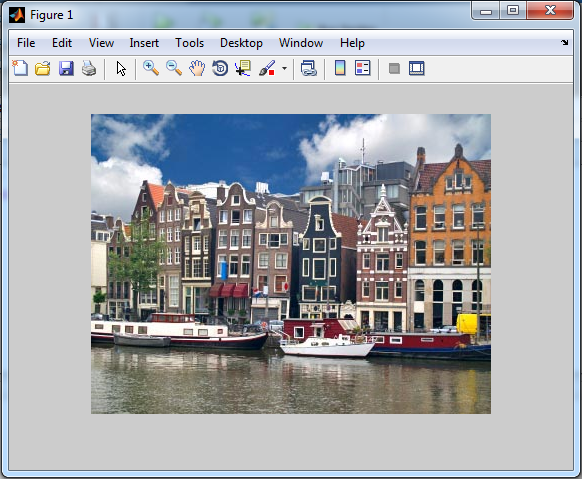
\includegraphics[width=0.75\textwidth]{images/ch7/holland_imshow.png}
    \caption{Utilizando \texttt{imread} & \texttt{imshow}}
    \label{fig:holland_imshow}
\end{figure}


La función \texttt{imshow} abre una nueva ventana (figure) y muestra la
imagen que ha sido guardada con anterioridad (ver figura \ref{fig:holland_imshow}). 
MATLAB dispone de otras funciones como \texttt{image} e \texttt{imagesc} que también muestran en pantalla las
imágenes, pero que suelen utilizarse más para la visualización en
análisis de datos.

\section{Operaciones básicas con imágenes}

\subsection{Operaciones aritméticas}

Recuerde que una imagen en MATLAB se almacena como una matriz de mxnxp
dimensiones, luego, es posible realizar operaciones aritméticas de suma,
resta y multiplicación sobre ella como una matriz común, tal como se ha
visto en Capítulo 2.

\subsubsection{Suma de un escalar}

Si sumamos una constante k a una matriz \textbf{A}, entonces cada
elemento de \textbf{A} se incrementa en k unidades, lo cual se
traduciría en un aumento del brillo en la imagen. Véase el ejemplo
siguiente:

\begin{matlab}
A=imread('imag.jpg');
k=50;
A=A+k;
imshow(A);
\end{matlab}

\begin{figure}[htbp]
    \centering
    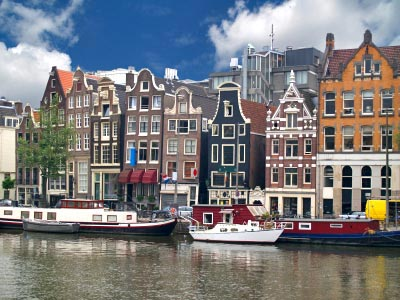
\includegraphics[width=0.75\textwidth]{images/ch7/holland_original.png}
    \caption{Imagen original}
    \label{fig:holland_original}
\end{figure}

\begin{figure}[htbp]
    \centering
    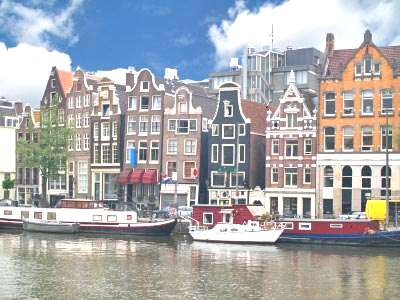
\includegraphics[width=0.75\textwidth]{images/ch7/holland_mas50.png}
    \caption{Imagen aumentada en 50 unidades}
    \label{fig:holland_mas50}
\end{figure}

La imagen \ref{fig:holland_original} corresponde a la original y en
la \ref{fig:holland_mas50} se muestra lo que resulta de aumentar
en 50 unidades cada uno de los pixeles que componen la imagen.

\subsubsection{Resta de un escalar}

Es evidente que la resta de un escalar es muy similar en interpretación
a la suma vista anteriormente, solo que en este caso cada elemento de la
matriz disminuye en un valor constante. Véase el ejemplo:

\begin{matlab}
A=imread('img.jpg');
k=80;
A=A-k;
imshow(A);
\end{matlab}

\begin{figure}[htbp]
    \centering
    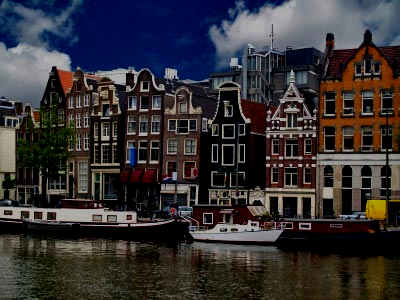
\includegraphics[width=0.75\textwidth]{images/ch7/holland_menos50.png}
    \caption{Imagen disminuida en 50 unidades}
    \label{fig:holland_menos50}
\end{figure}

\subsection{Conversión a escala de grises}

La escala de grises es una forma de representar imágenes digitales
utilizando solamente variaciones de grises, desde negro a blanco. \\

En MATLAB se dispone de la función \texttt{rgb2gray} para convertir una
imagen dada en el modelo de color RGB a una imagen en escala de grises.

\begin{matlab}
X=imread('img.png');
XG=rgb2gray(X);
imshow(XG);
\end{matlab}


\begin{figure}[htbp]
    \centering
    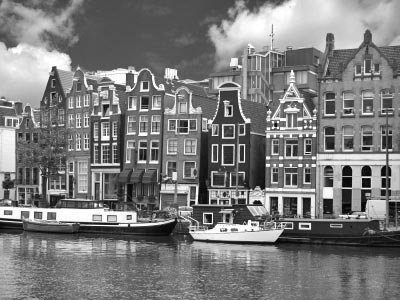
\includegraphics[width=0.75\textwidth]{images/ch7/holland_gris.png}
    \caption{Imagen en escala de grises}
    \label{fig:holland_gris}
\end{figure}

\subsection{Binarización de una imagen}

\subsection{Umbralización}\label{umbralizaciuxf3n}

\subsection{Detección de bordes}\label{detecciuxf3n-de-bordes}

\subsection{Removiendo ruido}\label{removiendo-ruido}
% \chapter{Introducción a las GUIs MATLAB}

Una interfaz gráfica de usuario (GUI) es un elemento gráfico que
contiene uno o más controles que están disponibles para interactuar con
el usuario mediante un entorno visual sencillo, el cual permite la
comunicación entre el usuario y el computador. Entre algunos de los
componentes más comunes de una GUI creada en MATLAB se tienen menús,
barras de herramientas, botones, menús desplegables, cajas de texto,
entre otros. \\

En las interfaces gráficas creadas en MATLAB pueden aprovecharse todas
las herramientas matemáticas y de ingeniería que proporciona MATLAB,
permiten además la manipulación de archivos de datos, así como la
interacción con otras GUIs y mostrar datos mediante tablas y gráficas de
gran calidad. \\

Generalmente las GUIs son programadas para que respondan a la
manipulación del usuario con una acción específica. Los controles
gráficos que componen una GUI están relacionados con una rutina de
programación, llamada callbacks en el entorno MATLAB, que se ejecuta
cuando sucede un determinado evento, que puede ser la entrada de
caracteres mediante el teclado, el clic de un botón del mouse, o
situarse sobre un objeto. \\

\section{¿Cómo crear una GUI en MATLAB?}

Una interfaz gráfica de usuario en MATLAB puede crearse de dos maneras,
a saber:

\begin{itemize}
\item
  Utilizando el entorno de desarrollo integrado (GUIDE - \emph{Graphical
  User Interface Development Environment}).
\item
  Código puro (programmatically GUI), es decir, utilizando sólo un
  script en el cual se colocarán las instrucciones necesarias para
  producir una interfaz gráfica.
\end{itemize}

¿Cuál es la mejor manera?, imposible dar una respuesta, dependerá mucho
de con cuál el desarrollador se sienta más cómodo. Utilizando GUIDE
puedes desarrollar interfaces gráficas rapidamente, arrastrando
controles y posicionándolos manualmente, para enseguida programar la
lógica principal. Con código puro quizá necesitas un poco más de
\emph{destreza} para colocar y organizar los elementos, pero vamos, nada
complicado en extremo. \\

En este capítulo, para presentar y conocer los objetos gráficos y sus
propiedades utilizaremos código puro, dado que esto permite proporcionar
toda la información necesaria a través del código mostrado, sin requerir
ningún otro tipo de archivo adicional.

\section{Los objetos gráficos en MATLAB}

Los objetos gráficos son los componentes visuales usados por MATLAB para
mostrar información o datos de manera gráfica, a la vez que pueden
permitir que el usuario interactúe mediante diversos controles. \\

Cada objeto tiene un identificador o referencia única llamada
\emph{handle}, mediante el cual se pueden manipular las propiedades del
objeto gráfico. \\

Los objetos gráficos están organizados de manera jerárquica tal como se
muestra en el siguiente diagrama:

\begin{figure}[htbp]
\centering
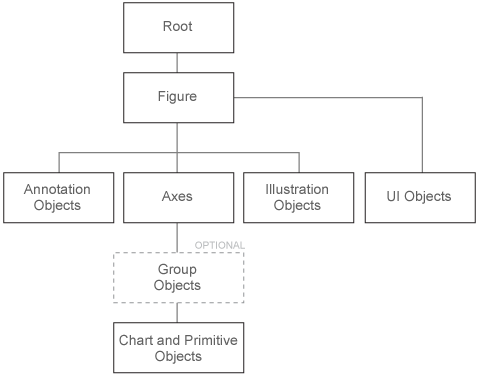
\includegraphics[width=0.6\textwidth]{images/ch8/objetos_graficos.png}
\caption{Jerarquía de los objetos gráficos en MATLAB}
\end{figure}

De manera general, la jerarquía sirve para determinar los objetos que
pueden contener a otro. Un objeto de mayor jerarquía puede contener a
otro de menor rango. Por ejemplo, un axes puede estar contenido dentro
de una ventana o \emph{figure}, viceversa imposible. \\

En el diagrama anterior puede notar que el objeto de mayor jerarquía es
el \emph{Root}, el cual refiere a la base de todo el sistema gráfico de
MATLAB. El objeto \emph{Root} no tiene un objeto padre, pero si puede
tener múltiples \emph{figures} o ventanas como hijos. \\


\begin{informacion}{Objetos padres e hijos}
En este capítulo y en cualquier referencia acerca de
interfaces gráficas encontrará que se hace referencia a
objetos \emph{padres} (\texttt{parent}) y objetos 
\emph{hijos} (\texttt{children}). Por la naturaleza de conceptos es
posible que tenga  una idea acertada de lo que refieren.
Un objeto es \emph{padre} de otro (objeto \emph{hijo}) 
sí este último está contenido dentro del primero. Entender esta relación
es importante,  dado que permita organizar y estructurar
de manera efectiva los controles  gráficos utilizando
\emph{contenedores} (usualmente paneles). Además, debe tomarse
 en cuenta para determinar el \emph{ciclo de vida} de un
objeto gráfico, así, es  pertinente saber que puede
borrar un \emph{hijo} sin afectar al \emph{padre}, pero si borra
 un \emph{padre} estará quitando, también, todos los
objetos que contenga.
\end{informacion}


\section{Propiedades de objetos: funciones \texttt{set} y \texttt{get}}

\section{Objeto \texttt{figure}}

En MATLAB cada interfaz gráfica está creada sobre un objeto
\texttt{figure}, en este elemento se añaden todos los controles gráficos
que componen la GUI. La forma más simple de definir un objeto figure se
ejemplifica enseguida:

\begin{matlab}
hFig = figure;
\end{matlab}

Donde \texttt{hFig} es el handle o referencia del elemento figure.\\

Es muy común que al momento de definir o crear un objeto figure, se
especifiquen algunas de sus propiedades con la sintaxis siguiente:

\begin{matlab}
hFig = figure('Propiedad', 'Valor',...);
\end{matlab}

A continuación se muestra un ejemplo característico:

\begin{matlab}
hFig = figure('NumberTitle','off',...
              'MenuBar','None',...
              'Name','Figure Ejemplo',...
              'Position',[200 200 300 300]);
\end{matlab}

Las propiedades más comunes de un elemento \texttt{figure} se muestran
en la tabla siguiente:

\begin{table}[h!]
\centering
% \rowcolors{1}{}{gray!20}
\begin{tabular}{p{3cm} p{10cm}}
\hline
\Centering\bfseries Propiedad & \Centering\bfseries Descripción \\
\hline
Color & Establece el color de figure. El valor puede establecerse mediante un vector de tres elementos en formato RGB \\
MenuBar & Oculta o muestra la barra de menús estándar de MATLAB \\
Name & Título mostrado en la ventana de la figura. El valor especificado es una cadena de caracteres \\
NumberTitle & Determina si la numeración de los elementos figure creada automáticamente por MATLAB será visible. El valor por defecto es on, para ocultar deberá especificarse off. \\
Position & Especifica el tamaño de la GUI y la posición relativa a la esquina inferior izquierda de la pantalla. El valor se establece mediante un vector de cuatro elementos cuya estructura es la siguiente: [Distancia de la izquierda, Distancia de la parte inferior, Ancho, Alto]; \\
Resize & Determina si puede modificarse el tamaño de la GUI utilizando el mouse. Los valores aceptados son: off y on, siendo este último el valor por defecto. \\
Toolbar & Muestra o borra el menú de herramientas del objeto figure. \\ 
Units & Unidad de medida que se utilizará para interpretar el vector de la propiedad position. Los valores disponibles son: centimeters, characters, inches, normalized, point y pixels. Siendo este último el valor por defecto. \\
Visible & Establece si la GUI es visible. Valores: on y off. \\
\hline
\end{tabular}
\caption{aaaaa}
\end{table}


\section{Controles gráficos (\texttt{uicontrol})}

Los elementos gráficos son todos aquellos componentes que conforman una
interfaz gráfica y que están contenidos dentro de una ventana o
\texttt{figure}. Estos elementos pueden ser campos de texto, botones,
listas desplegables o cualquier otro tipo de elemento gráfico que
permita una interacción con el usuario. \\

En esta sección vamos a ver cómo crear los controles básicos utilizando
la función \texttt{uicontrol}, misma que tiene una sintaxis como sigue:

\begin{matlab}
hCont = uicontrol(Parent, 'Style', 'tipo de control',...
                  'Propiedad', 'Valor');
\end{matlab}

Donde \texttt{Parent} es un objeto gráfico de mayor jerarquía (como
puede ser un panel o un frame/ventana) en el cual va a estar contenido
el control gráfico. La propiedad \texttt{style} define el tipo de
control gráfico a desarrollar. Luego, se pueden pasar varios
\emph{argumentos pareados} o de tipo \texttt{Nombre-Valor}que definan
otras características del control como pueden ser la posición, el color,
el contenido o valor, o bien la asociación a una función que maneje el
evento \emph{disparado} cuando el usuario o la lógica del programa
interaccionen con este. En \texttt{hCont} se guardará la referencia al
objeto creado, mediante la cual posteriormente podemos acceder o
modificar sus propiedades con las funciones \texttt{get} y \texttt{set}. \\ 

En la siguiente tabla se muestran los posibles tipos de control que
pueden ser pasados en la propiedad \texttt{style}.

\begin{table}[h!]
\centering
% \rowcolors{1}{}{gray!20}
\begin{tabular}{p{3cm} P{10cm}}
\hline
\Centering\bfseries Tipo (style) & \Centering\bfseries Control gráfico \\
\hline

checkbox & 
\includegraphics[scale=0.75]{images/ch8/checkbox.png} \\
edit & 
\includegraphics[scale=0.75]{images/ch8/edit.png} \\
listbox & 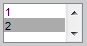
\includegraphics[scale=0.75]{images/ch8/listbox.png} \\
popupmenu & 
\includegraphics[scale=0.75]{images/ch8/popupmenu.png} \\
pushbutton & 
\includegraphics[scale=0.75]{images/ch8/pushbutton.png} \\
radiobutton & 
\includegraphics[scale=0.75]{images/ch8/radiobutton.png} \\
slider & 
\includegraphics[scale=0.75]{images/ch8/slider.png} \\
text & 
\includegraphics[scale=0.75]{images/ch8/text.png} \\
togglebutton & 
\includegraphics[scale=0.75]{images/ch8/togglebutton.png} \\

\hline
\end{tabular}
\caption{Valores especiales}
\end{table}


La siguiente tabla resume algunas de las \emph{propiedades pareadas} más
utilizadas, que pueden pasarse como argumentos a la función \texttt{uicontrol}:

\begin{table}[h!]
\centering
% \rowcolors{1}{}{gray!20}
\begin{tabular}{p{3cm} p{9cm}}
\hline
\Centering\bfseries Propiedad & \Centering\bfseries Descripción \\
\hline
BackgroundColor & Establece el color del control. El valor puede establecerse mediante un vector de tres elementos en formato RGB. \\

Callback & Función que se ejecuta cuando el usuario interactúa con el control gráfico. El valor pasado puede ser la referencia a una función, por ej: \texttt{@mifuncion} \\

FontName & Fuente a utilizar. Debe ser un string con el nombre de la fuente, la cual debería estar instalada. \\

FontSize & Tamaño de fuente. Valor numérico en las unidades dadas por \texttt{FontUnits} \\

FontUnits & Unidad utilizada para interpretar el valor numérico de \texttt{FontSize} \\

FontWeight & Aspecto de la fuente, puede ser \texttt{normal} o \texttt{bold} (negritas), por default es \texttt{normal} \\

ForegroundColor & Color de la fuente utilizada en control gráfico \\

Parent & Objeto gráfico padre. El valor debe ser un handle o referencia a un objeto gráfico de mayor jerarquía. \\

Position & Especifica el tamaño del control y la posición relativa a la esquina inferior del objeto padre. El valor se establece mediante un vector de cuatro elementos cuya estructura es la siguiente: \texttt{[Distancia de la izquierda, Distancia de la parte inferior, Ancho, Alto]} \\

String & Cadena de texto que se muestra en el control. El valor pasado como argumento puede ser cualquier string. \\ 

Units & Unidad de medida que se utilizará para interpretar el vector de la propiedad \texttt{position}. 
Los valores disponibles son: centimeters, characters, inches, normalized, point y pixels. Siendo este último el valor por
defecto. \\

Visible & Establece si el control es visible. Valores: \texttt{on} y \texttt{off}. \\

\hline
\end{tabular}
\caption{Valores especiales}
\end{table}


\subsection{Check Box}\label{check-box}

El Check Box es un elemento gráfico que sirve como casilla de
verificación, para indicar dos posibles estados: activado/desactivado o
falso/verdadero, como un tipo de check list. Vea el siguiente código:


\begin{matlab}
figure('MenuBar','none',...
    'Position',[100 100 200 100]);

uicontrol('style','checkbox',...
    'string','Rojo',...
    'Position',[10 10 80 20],...
    'Callback',@cambia_color);

    function cambia_color(src, ~)
        if get(src,'Value') == true
            set(gcf,'Color','r');
        else
            set(gcf,'Color',0.8*ones(1,3));
        end
    end
end
\end{matlab}

El código anterior crea una ventana de 200x100 pixeles que contiene un
check box con el string \texttt{Rojo}. Además, puede notar que a la
propiedad \texttt{Callback} se la pasa como argumento una función
\verb|cambia_color| que cada vez que es ``llamada'' cambia el color
de fondo de la ventana: a rojo cuando se activa el check box y al color
por default cuando se desactiva.

\begin{figure}[htbp]
\centering
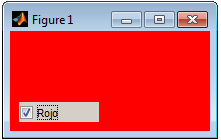
\includegraphics[width=0.4\textwidth]{images/ch8/checkbox_example.png}
\caption{Checkbox}
\end{figure}

\subsection{Edit Text}\label{edit-text}

Un \emph{edit text} es un campo de texto editable en el cual se puede
introducir información en forma de texto, es el clásico \emph{input} que
todos conocemos, como la barra de búsqueda en un buscador de internet o
aquellos cuando rellenamos un formulario \emph{online}.

\subsection{List Box}\label{list-box}

\subsection{Pop-up Menu}\label{pop-up-menu}

\subsection{Push Button}\label{push-button}

\subsection{Radio Button}\label{radio-button}

\subsection{Slider}\label{slider}

\subsection{Static Text}\label{static-text}

\subsection{Toggle Button}\label{toggle-button}


\section{Paneles}\label{paneles}

\section{Axes}\label{axes}

\section{Tablas}\label{tablas}

% \chapter{Programación orientada a objetos}

\section{Conceptos básicos de la POO}

La programación orientada a objetos (POO) es un paradigma de
programación que utiliza objetos como parte esencial de sus
interacciones, para el desarrollo de aplicaciones y soluciones
tecnológicas. La POO está soportada por técnicas de programación tales
como la herencia, el polimorfismo, el encapsulamiento, entre otras, cada
una de ellas proporciona herramientas que han permitido la proliferación
de este modelo de programación en las últimas décadas. Actualmente
existen una variedad de lenguajes que soportan la POO, siendo los más
conocidos C++, Java y C\#. \\

El soporte \emph{moderno} de MATLAB para la POO es relativamente nuevo,
siendo introducido a partir de la versión 7.6 (R2008a) con notables
carencias respecto a los lenguajes de referencia en ese aspecto, pero
evidentemente la mejora desde entonces ha sido considerable. \\

\begin{informacion}{Sobre POO}
Con soporte \emph{moderno} se hace alusión a la notación
actual que se  utiliza en la definición de clases, por
ejemplo \texttt{classdef} para crear  una clase. Puesto
que antes de la implementación de esta notación,  existía
la posibilidad de programar orientado a objetos haciendo uso
 de algunos \emph{artilugios}, como el colocar la clase
(definida mediante  una función que hacía lo de un
\emph{constructor} de la clase) y sus  métodos dentro de
una carpeta cuyo nombre debería ser el de la clase  misma
anteponiéndole un arroba (@).
\end{informacion}

\subsection{Clases y objetos}

Una clase es una definición de las propiedades y/o características de un
determinado tipo de objetos, es decir, un modelo particular que sirve
para crear objetos bajo esas mismas especificaciones. \\

Un objeto es la representación concreta derivada de una clase que está
provisto de atributos y métodos, o en términos más formales: un objeto
es la instancia de una clase. \\

A manera de ejemplo y un contexto más apegado a la realidad,
consideremos a los perros como una determinada clase, es sencillo
hacernos la idea de cómo es un perro y cuáles son sus características y
apariencia general; luego, el perro que tenemos en casa (en caso de que
así sea) es una instancia de esa clase o un objeto de la clase perro,
con características más particulares pero que no les excluyen de ser un
perro.

\subsection{Atributos}

Los atributos son las propiedades asociadas a una clase de objetos.
Siguiendo con el ejemplo de los perros, estos tienen atributos como el
tamaño, color, raza, temperamento, etc. Es común en la POO diferenciar
entre dos tipos de atributos acorde a su accesibilidad: los privados y
los públicos. Los privados son atributos disponibles solo dentro de la
definición de la clase, en cambio los públicos son accesibles desde
cualquier otra clase o fichero de instrucciones.

\subsection{Métodos}

Los métodos de una clase de objetos son algoritmos o bloques de
programación que determinan el comportamiento de un objeto. Por lo
general los métodos se usan para modificar los atributos de un objeto o
bien generar un nuevo evento. En MATLAB los métodos son definidos
mediante funciones.

\subsection{Eventos}

Un evento es la \emph{reacción} que tiene un objeto resultante de la
interacción con el usuario o bien mediante la ejecución de los métodos.

\section{Definiendo clases en MATLAB}

Las clases son el \emph{alma} de la POO, y suelen definirse en ficheros
únicos. En MATLAB pueden crearse utilizando un fichero \verb|*.m| ordinario y
colocando en este la sintaxis para la definición de una clase, la cual
se muestra enseguida:

\begin{matlab}
classdef nombreClase
    % Descripción de la clase
    
    properties
        % Atributos
    end
    
    methods
        % Métodos
    end
    
end
\end{matlab}

En la mayoría de los lenguajes que soportan POO se utiliza la palabra
clave class para definir una clase, pero en MATLAB \texttt{class} se
utiliza para identificar el tipo o clase de una variable u objeto, y en
cambio se utiliza \texttt{classdef} para definir una clase. Los
atributos de una clase se definen en un bloque properties-end, y pueden
simplemente ser declarados sin asignación de valores. Los métodos de la
clase se especifican dentro de un bloque methods-end, incluyendo al
constructor de la clase.

\subsection{El constructor de la clase}

El constructor de una clase es parte esencial de la misma y en este se
definen los argumentos o parámetros formales necesarios para crear un
objeto de la clase, de ahí su importancia. En MATLAB el constructor se
considera, de manera no estricta, un método y por tanto se define dentro
del bloque correspondiente a los métodos. Así pues, incluyendo al
constructor la definición de una clase sería algo similar a:

\begin{matlab}
classdef nombreClase
    % Descripción de la clase
    
    properties
        % Atributos
    end
    
    methods
        function obj = nombreClase(args)
           % Constructor de la clase 
        end
        % ...
        % Métodos
        % ...
    end
    
end
\end{matlab}

En lo anterior obj es, dentro la definición de la clase, una referencia
al objeto instanciado y es obligatorio el colocarlo como \emph{valor de
salida} (en la terminología de funciones); claro que el identificador
\texttt{obj} puede cambiarlo por cualesquiera otro de su comodidad
(\texttt{this} o \texttt{self} podrían ser buenas opciones, claro, mucho
influye el hecho de haber programado en otro lenguaje de POO en este
tipo de \emph{adopciones} de estilo). Tal como se ejemplifica, el nombre
de la función que funge como constructor debe ser el mismo que el de la
clase, además deben especificarse los argumentos que se utilizarán para
crear un objeto.

\section{La clase Persona, una primera aproximación}

En la sección anterior hemos visto la sintaxis para definir una clase,
pero como casi todo siempre es mejor asociar un concepto teórico con un
ejemplo concreto. Para tal fin crearemos la clase Persona, de naturaleza
muy sencilla pero significativa. \\

En principio vamos a definir las propiedades o atributos que habrán de
caracterizar a un objeto de la clase Persona, así pues, dada la
simplicidad del caso solamente utilizaremos el nombre y la edad para
\emph{construir} un objeto de esta clase. Por ahora no definiremos
método alguno, solamente el constructor de la clase. Véase la definición
resultante:

\begin{matlab}
classdef Persona
    % Persona
    %
    % Ejemplo :
    %           p1 = Persona('Jorge',22);
    %           p2 = Persona('Anna',28);          
    %
    
    properties % Atributos de la clase
        nombre;
        edad;
    end
    
    methods
        function obj = Persona(nombre,edad) % Constructor
            obj.edad=edad;
            obj.nombre=nombre;
        end
    end
    
end
\end{matlab}

Para \emph{testear} una clase podemos crear un script en donde colocar
las instrucciones necesarias para crear un objeto de la misma. No
obstante, por ahora haremos esto en la ventana de comandos de la
siguiente manera:

\begin{matlab}
>> p = Persona('Ana',25);
>> whos
  Name      Size            Bytes  Class      Attributes
  p         1x1               118  Persona        
\end{matlab}

% \chapter{Recomendaciones generales}\label{recomendaciones-generales}

\section{Escribiendo código legible}\label{escribiendo-cuxf3digo-legible}

La legibilidad cuenta, claro que sí. Una frase de Abelson y Sussman, en
el libro Estructura e interpretación de Programas de Computadora, lo
resume de forma notable: \emph{Los programas deben escribirse para que
los lean las personas y sólo de forma circunstancial para que los
ejecuten las máquinas.} \\

De modo que cuando se escribe código, en cualquier lenguaje de
programación, es importante estructurar los programas de una forma que
resulte entendible para cualquier individuo. Entonces, se deben
desarrollar lineas de código pensando en que en algún momento alguien
más tratará de entenderlo (sí, aun cuando esto sea poco probable). \\

A continuación se listan algunas recomendaciones básicas para
estructurar un programa:

\subsection{Nombres de variables autodescriptivos}\label{nombres-de-variables-autodescriptivos}

Siempre que sea posible es preferible utilizar nombres de variables
autodescriptivos, aún cuando estos resulten un poco extensos. La
ganancia en legibilidad lo compensa todo, por ejemplo, es preferible
tener:

\begin{matlab}
fuerza = 10;
area = 20;
presion = fuerza/area;
\end{matlab}

a simplemente colocar:

\begin{matlab}
f = 10;
a = 20;
p = f/a;
\end{matlab}

\subsection{Indentación del código}\label{indentacion-del-codigo}

Una buena indentación del código permite distinguir los diversos bloques
de programación. Actualmente el editor de MATLAB proporciona
herramientas que facilitan esta tarea, simplemente seleccionando el
código y presionando Ctrl + I para un \emph{indentado inteligente}. Note
las diferencias entre los códigos siguientes:

\begin{matlab}
k = 1;
while true
if rem(k,2)==0
disp('Par');
else
disp('Impar');
end
k = k + 1;
end


k = 1;
while true
    if rem(k,2)==0
        disp('Par');
    else
        disp('Impar');
    end
    k = k + 1;
end
\end{matlab}

\subsection{Documentación del
código}\label{documentaciuxf3n-del-cuxf3digo}

\subsection{Espacios}\label{espacios}

\section{Optimizando el código}\label{optimizando-el-cuxf3digo}

\subsection{Pre-asignación
(pre-allocation)}\label{pre-asignaciuxf3n-pre-allocation}

Una de las grandes ¿ventajas? de MATLAB es su \emph{tipado dinámico}

\subsection{Vectorización}\label{vectorizaciuxf3n}


\end{document}